\documentclass[12pt]{article}

\usepackage[utf8]{inputenc}
\usepackage{amsmath}
\usepackage{amssymb}
\usepackage{caption}
\usepackage{color}
\usepackage{float}
\usepackage{graphicx}
\usepackage{listings}
\usepackage{physics}
\usepackage{textcomp}


\setlength{\parindent}{3em}
\setlength{\parskip}{1.5em}
\renewcommand{\baselinestretch}{1.5}


\title{
	\Large{CSE-322}\\
	\Large{Report on NS2}
	\endgraf\bigskip
}

\author{
    \Large{Submitted By-}\\
	\Large{Waqar Hassan Khan (1505107)}\\
	\Large{Ahmed Nafis Fuad (1505113)}\\
}

\date{}

\begin{document}

%--------------------------------------------------cover page	
\maketitle

\section*{}
\begin{figure}[h]
	\centering
	
	\captionsetup{justification=centering}
	
\includegraphics[width = 0.1\textwidth]{image/buet.png}
	\caption*{
		\Large{Department of Computer Science and Engineering}
		\\
		\Large{Bangladesh University of Engineering and Technology}
		\\
		\Large{(BUET)}
		\\
		\Large{Dhaka 1000}
		\\
		\Large{\today}
	}
	
\end{figure}
%--------------------------------------------------cover page

\newpage
\tableofcontents
\newpage



%---------------------------------------------------------------intro
\section{Network Topologies Under Simulation}
\begin{itemize}
	\item wireless 802.11 - mobile
	\item wireless 802.15.4 - static
\end{itemize}

\section{Parameters Under Variation}
\subsection{wireless 802.11 - mobile}
\begin{itemize}
	\item number of nodes
	\item number of flow
	\item number of packets sent per second
	\item speed of node
\end{itemize}

\subsection{wireless 802.15.4 - static}
\begin{itemize}
	\item number of nodes
	\item number of flow
	\item number of packets sent per second
	\item coverage area
\end{itemize}

\section{Modifications Made in The Simulator}
\begin{itemize}
    \item change in tcp.cc : the RTO(re-transmission timeout) calculation implemented in ns2.35 \textrightarrow tcp \textrightarrow tcp.cc follows Jacobson Algorithm. The calculation has been changed.
    
    In Jacobson algorithm, in order to calculate the current RTO, TCP sender need to maintain two variables, SRTT and RTTVAR. After completing the first RTT,\\
    $SRTT_1 = RTT_1$\\
    $RTTVAR_1 = RTT_1/2$\\
    
    for the next updates,\\
    $SRTT1_{n+1} = (1 - \alpha) * SRTT_n + \alpha * RTT_{n+1}$\\
    $RTTVAR_{n+1} = (1 - \beta) * RTTVAR_n + \beta*\abs{SRTT_{n+1} - RTT_{n+1}})$\\
    $RTO_{n+1} = SRTT_{n+1} + 4 * RTTVAR_{n+1}$\\
    
    The calculation has been changed according to a paper,
    a variable $K$ - RTT's rate of change is required by the following formula
    $K_{n+1} = \abs{RTT_{n+1} - RTT_n} / RTT_n$\\
    if K\textgreater 1 then K=1.\\
    unlike Jacobson algo $\alpha$ and $\beta$ would be changed\\
    $\alpha_{n+1} = \alpha_0 * (1 + K_{n+1})$\\
    $\beta_{n+1} = \beta_0 * (1 - K_{n+1})$\\
    the values of $\alpha_0=1/8$ and $\beta_0=1/4$\\
    $SRTT1_{n+1} = (1 - \alpha_{n+1}) * SRTT_n + \alpha_{n+1} * RTT_{n+1}$\\
    $RTTVAR_{n+1} = (1 - \beta_{n+1}) * RTTVAR_n + \beta_{n+1}*\abs{SRTT_{n+1} - RTT_{n+1}})$\\
    $RTO_{n+1} = SRTT_{n+1} + 4 * RTTVAR_{n+1}$\\
    
    the change improves the retransmition of packet, it decreases.\\
    
    \item DSDV protocol has been modified. The DVR(distance vector routing) algorithm had a problem of "count to infinity", in order to fix it DSDV uses a sequence number. Here DSDV has been converted to DVR by omitting the codes associated with sequence number -> as a result throughput has decreased, possibly there are some entries got missing. \\
\end{itemize}
%---------------------------------------------------------------


%---------------------------------------------------------------
%graphs

\newpage
\section{Graphs}
\subsection{802.11}

\title{Variation in Number of Nodes}
\begin{figure}[H]
	\centering
	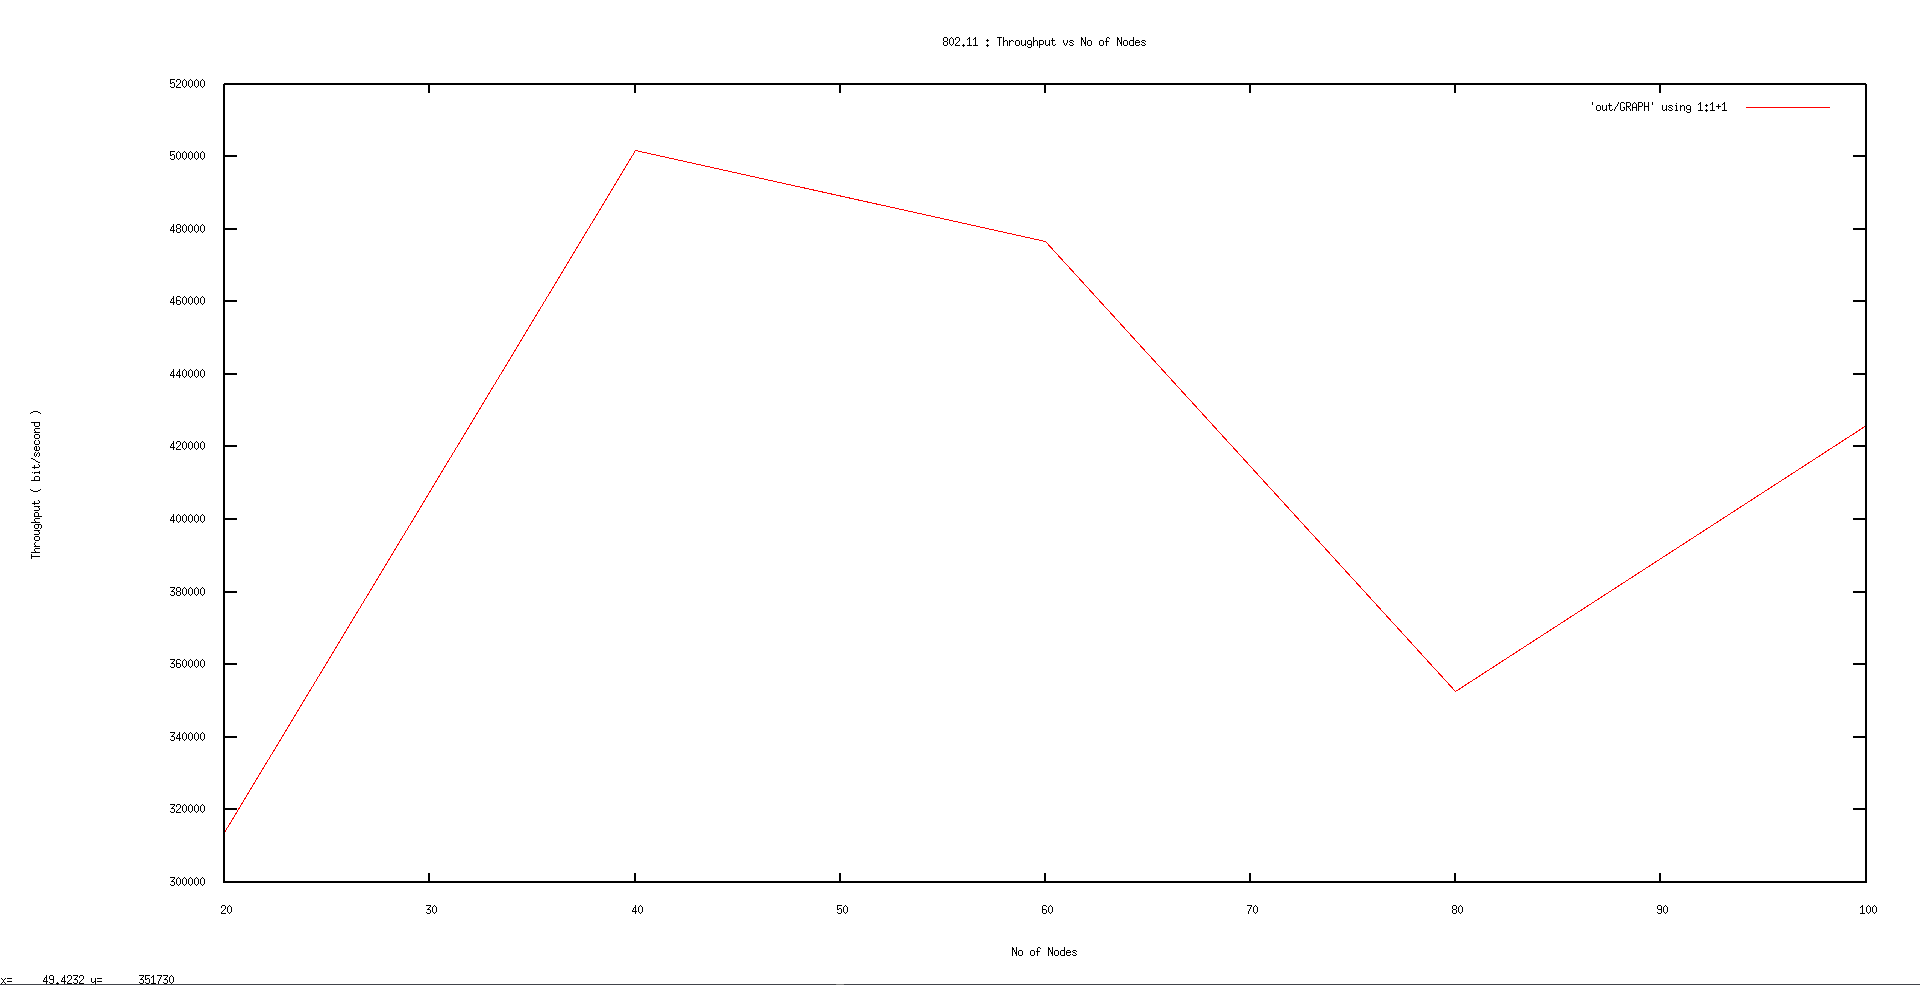
\includegraphics[scale=	0.26]{image/802.11/Throughput_vs_nodes.png}
\end{figure}

\begin{figure}[H]
	\centering
	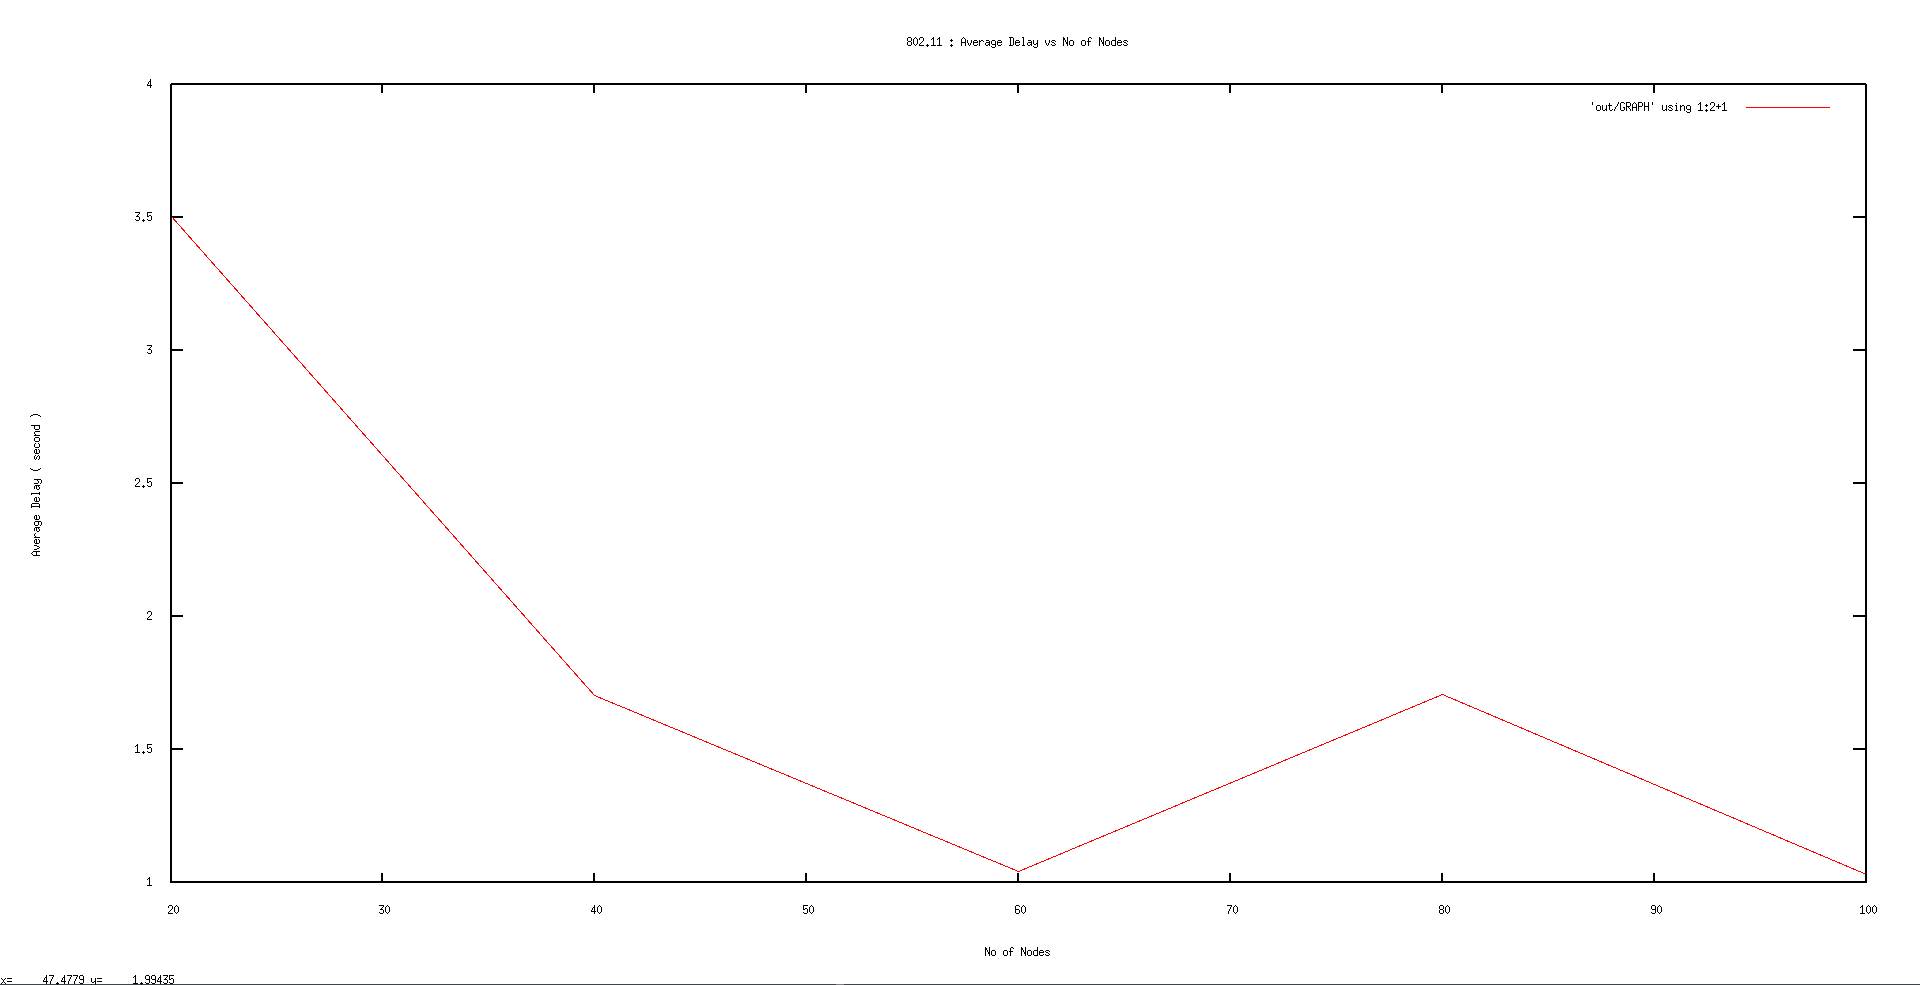
\includegraphics[scale=	0.26]{image/802.11/Averagedelay_vs_nodes.png}
\end{figure}

\begin{figure}[H]
	\centering
	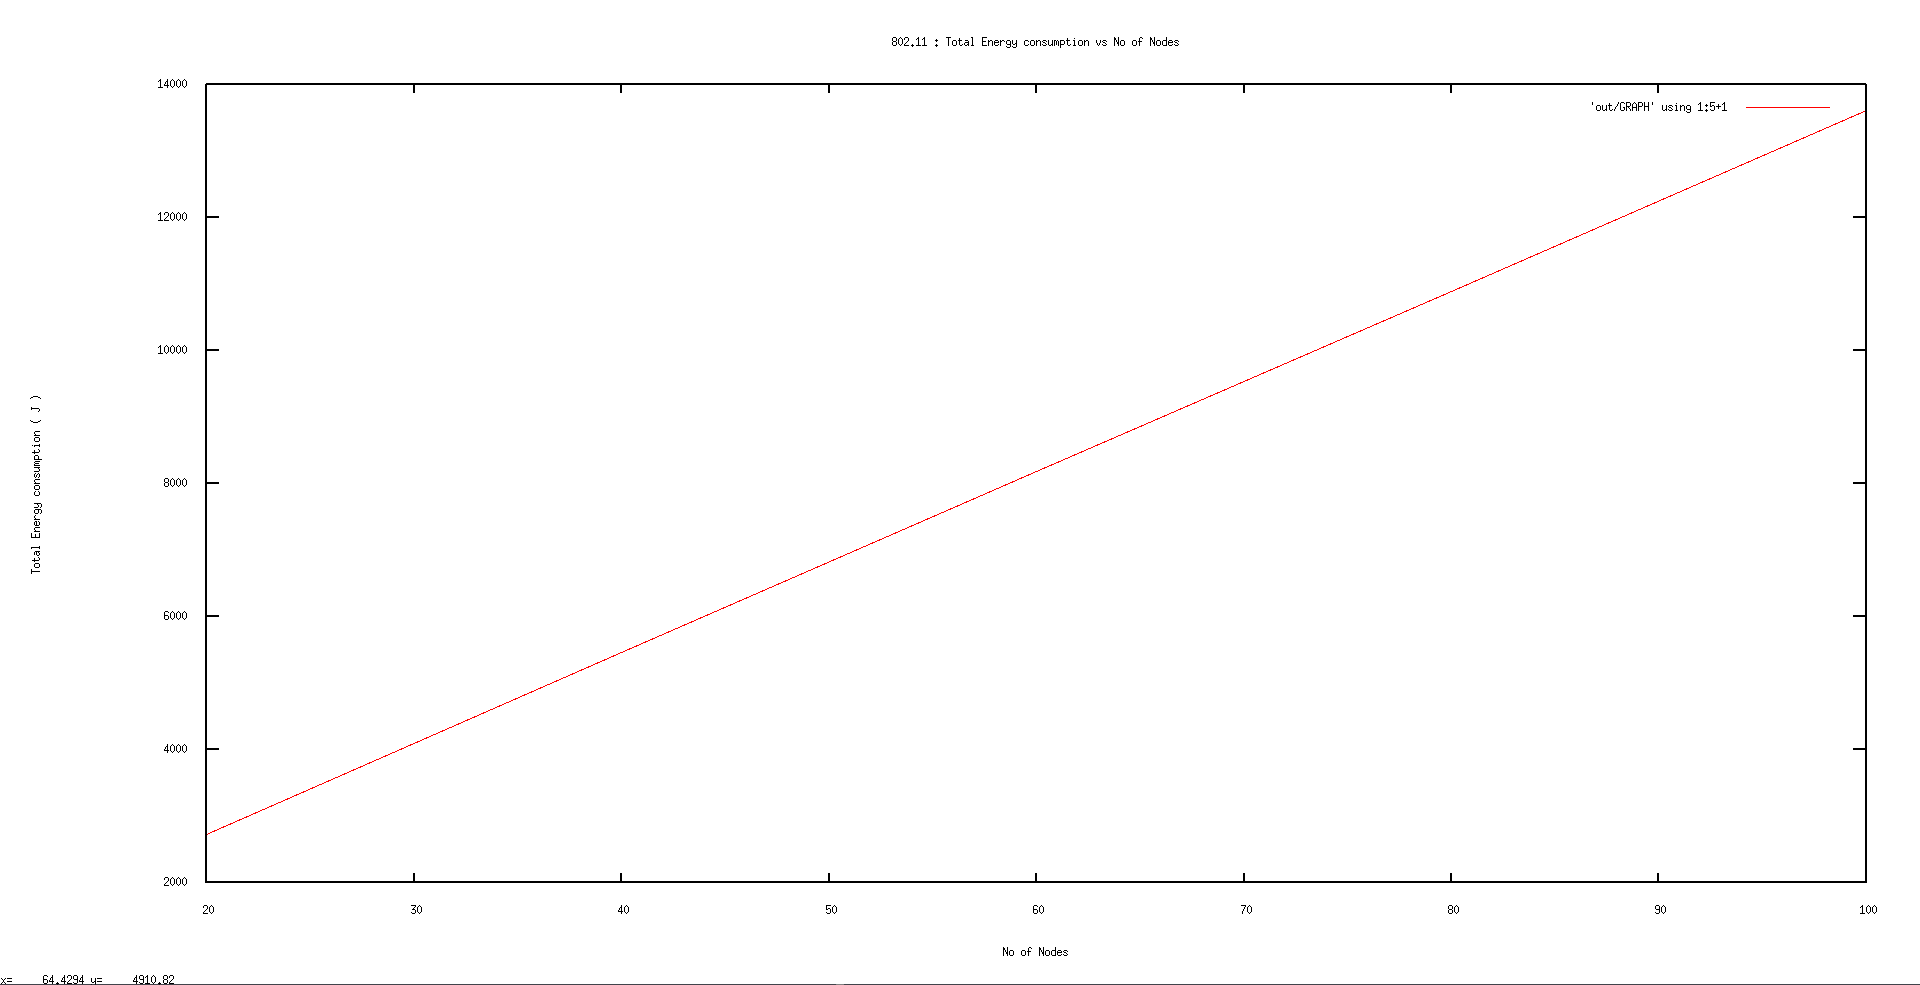
\includegraphics[scale=	0.26]{image/802.11/Energyconsumption_vs_nodes.png}
\end{figure}

\begin{figure}[H]
	\centering
	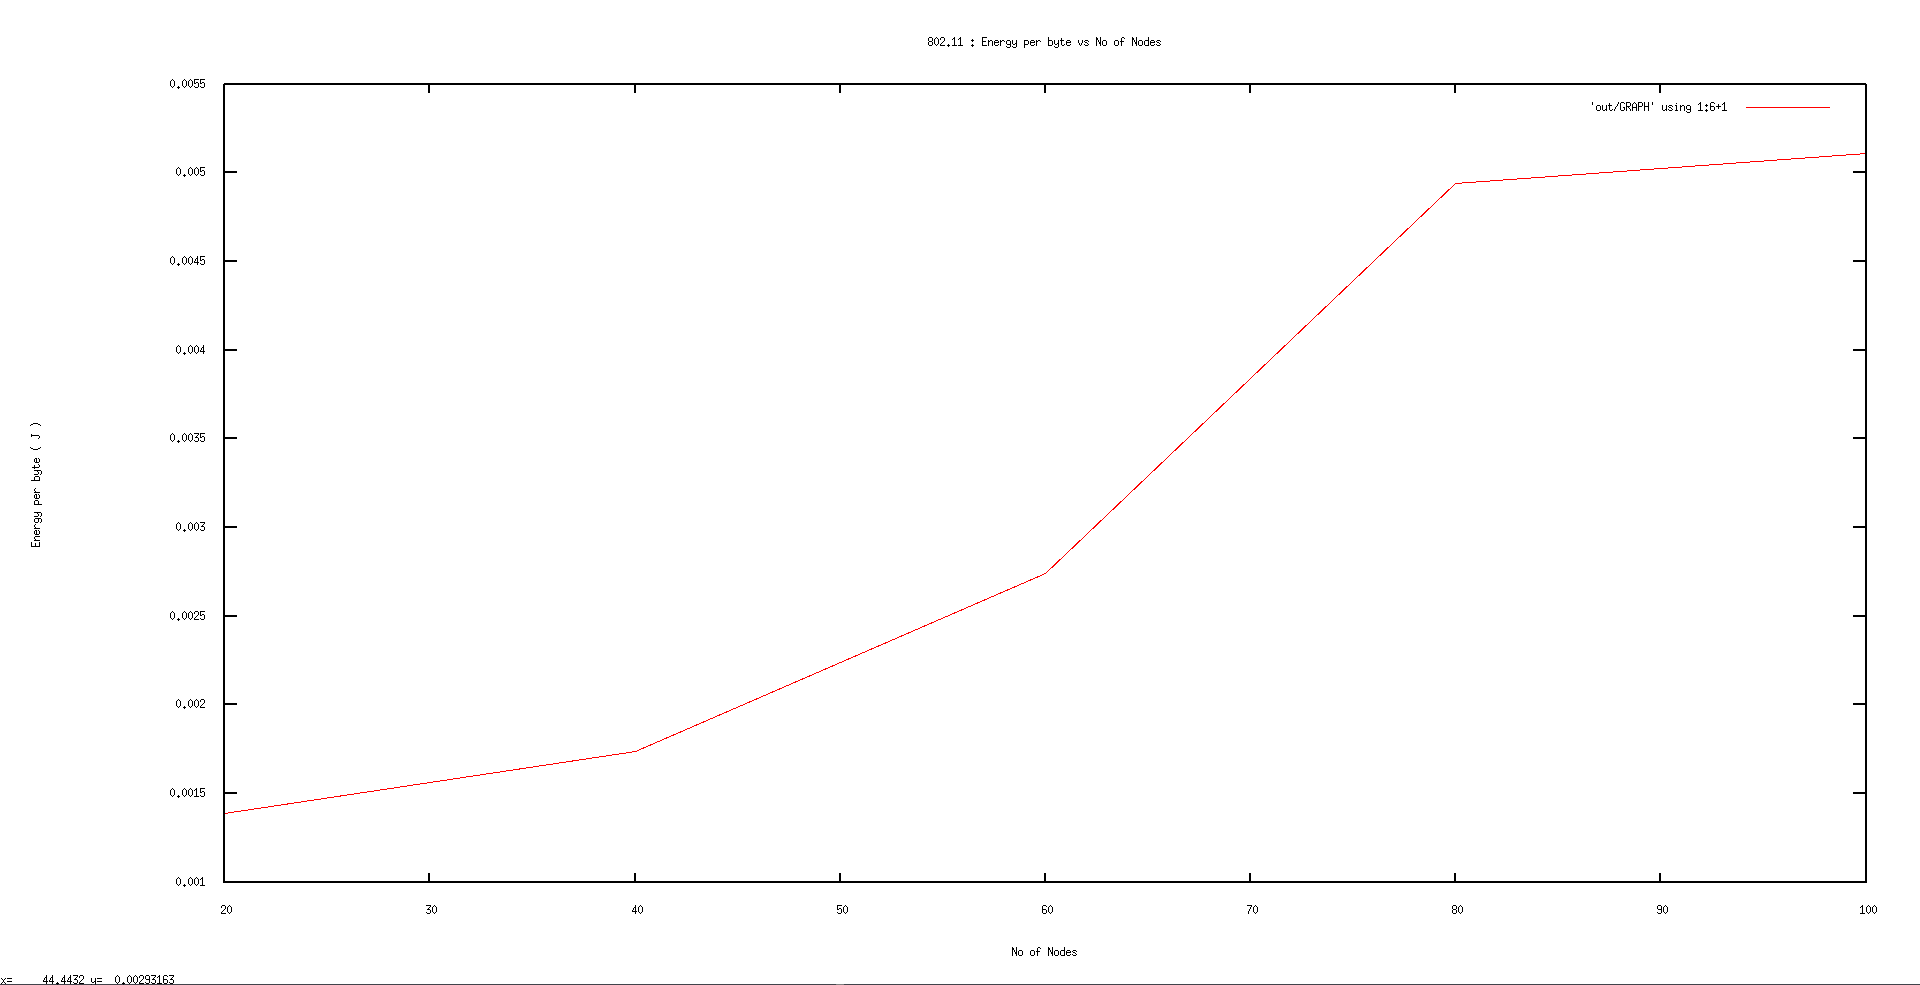
\includegraphics[scale=	0.26]{image/802.11/Energyperbytes_vs_nodes.png}
\end{figure}

\begin{figure}[H]
	\centering
	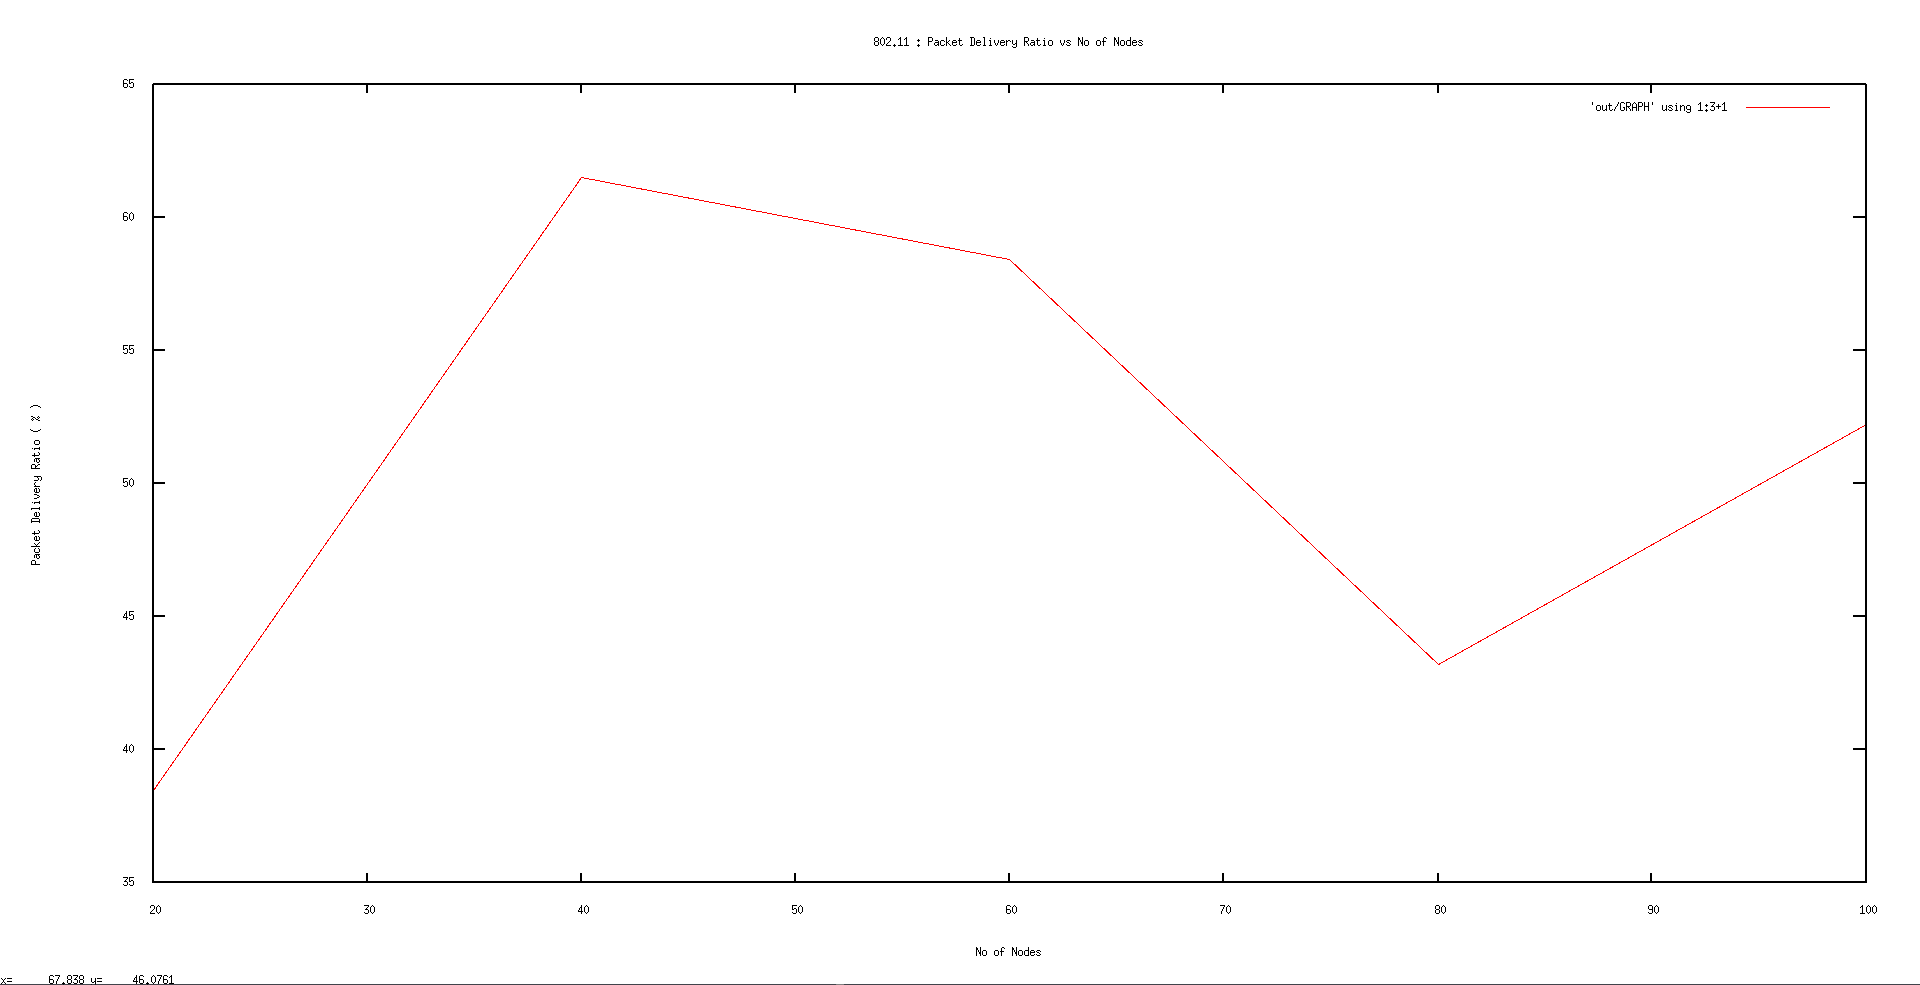
\includegraphics[scale=	0.26]{image/802.11/Packetdeliveryratio_vs_nodes.png}
\end{figure}

\begin{figure}[H]
	\centering
	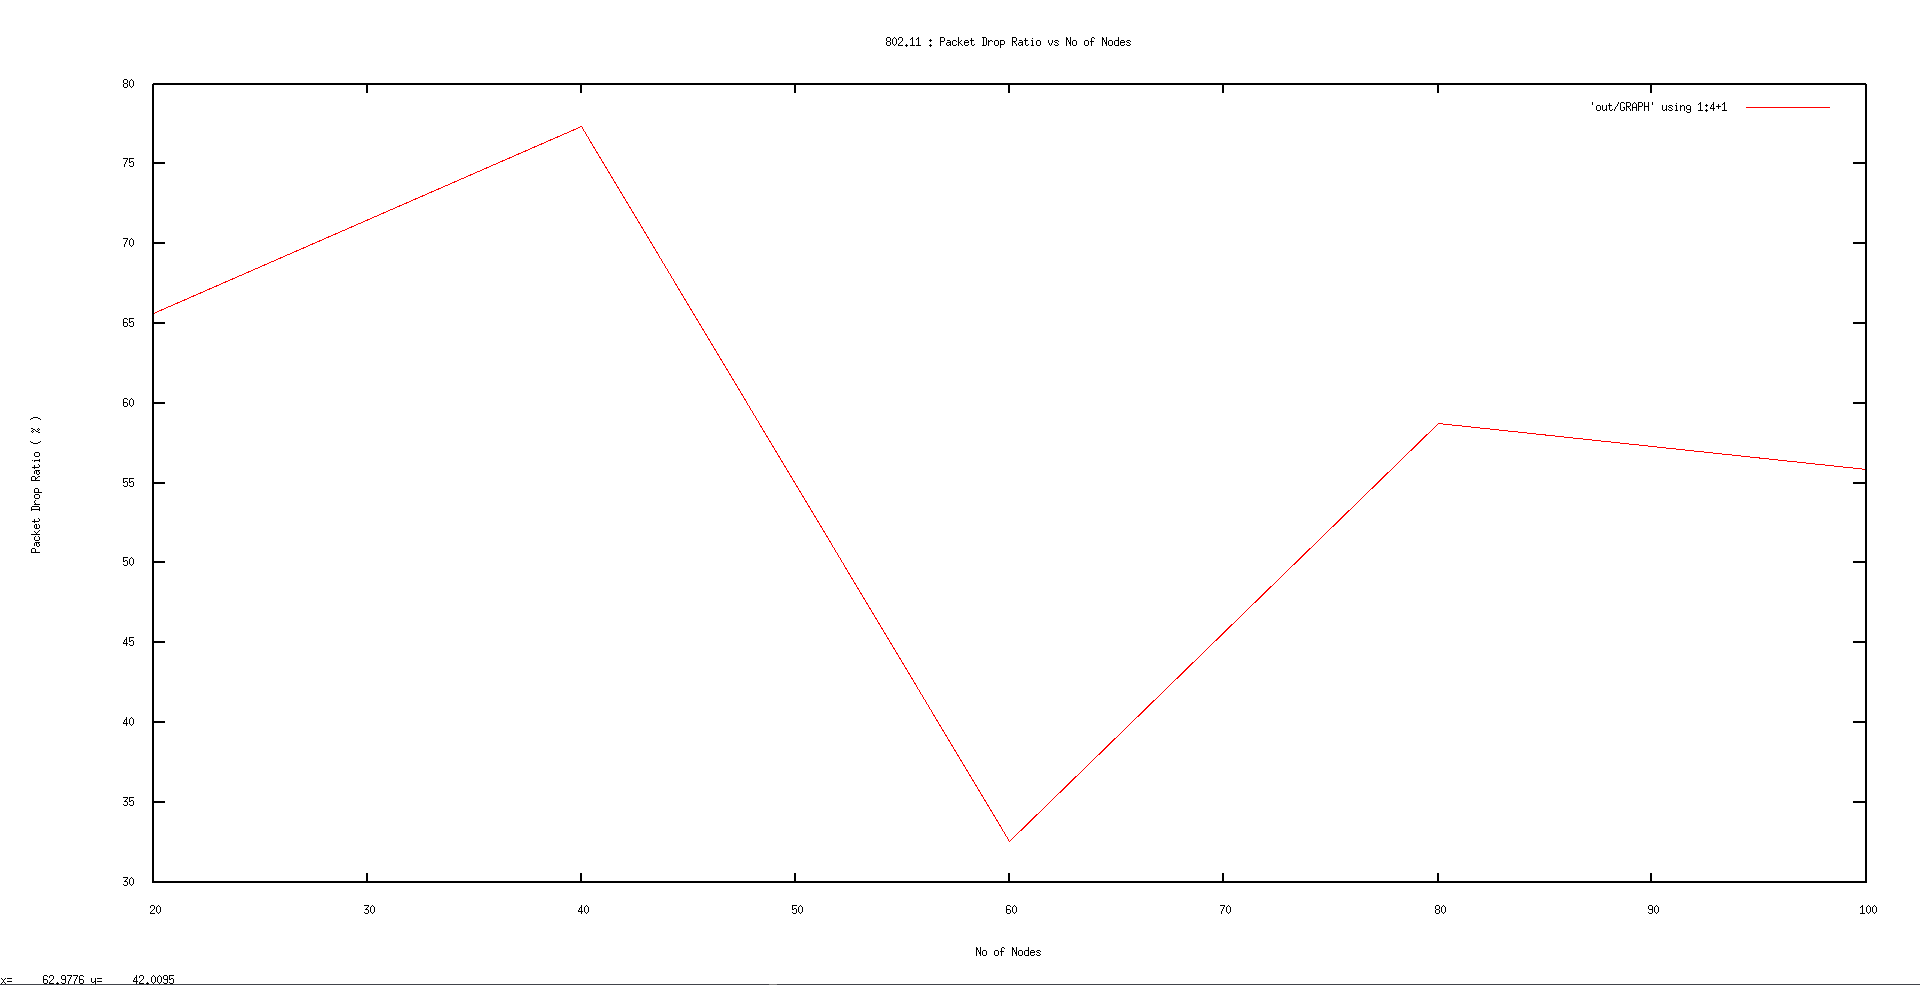
\includegraphics[scale=	0.26]{image/802.11/Packetdropratio_vs_nodes.png}
\end{figure}


\newpage
\title{Variation in Number of Flow}
\begin{figure}[H]
	\centering
	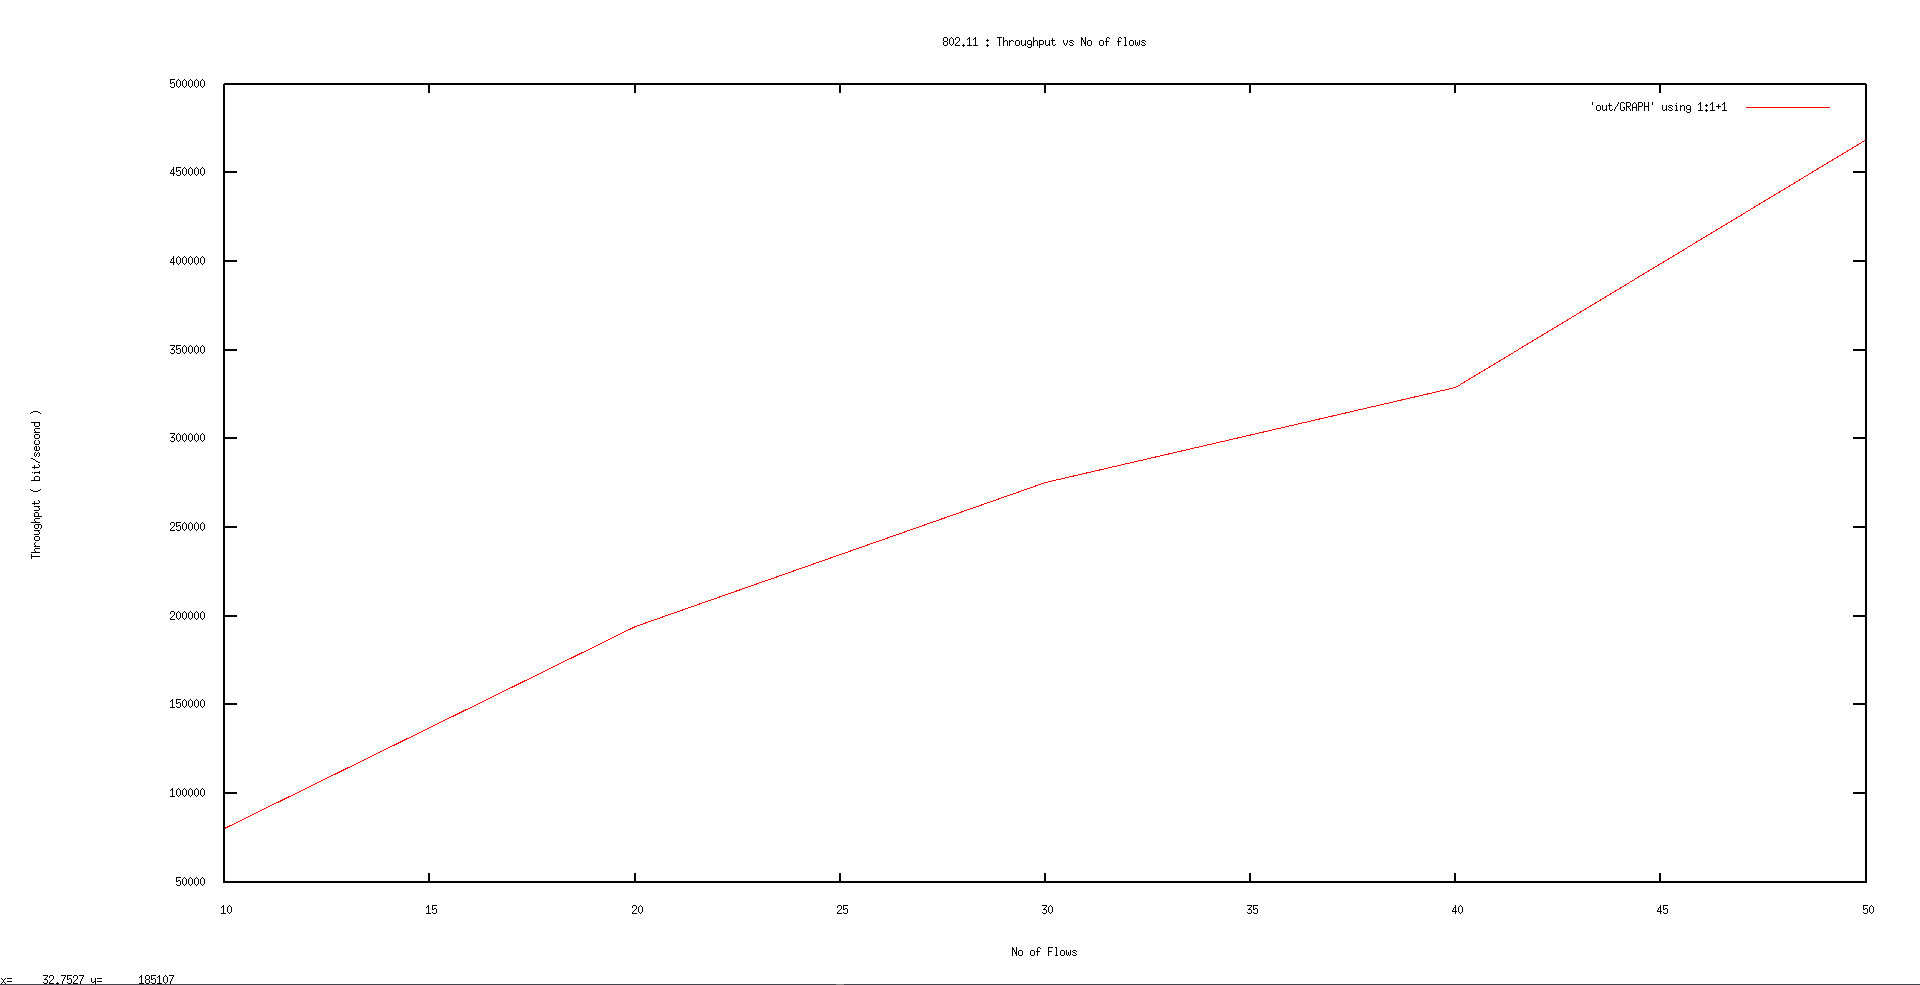
\includegraphics[scale=	0.26]{image/802.11/Throughput_vs_flows.png}
\end{figure}

\begin{figure}[H]
	\centering
	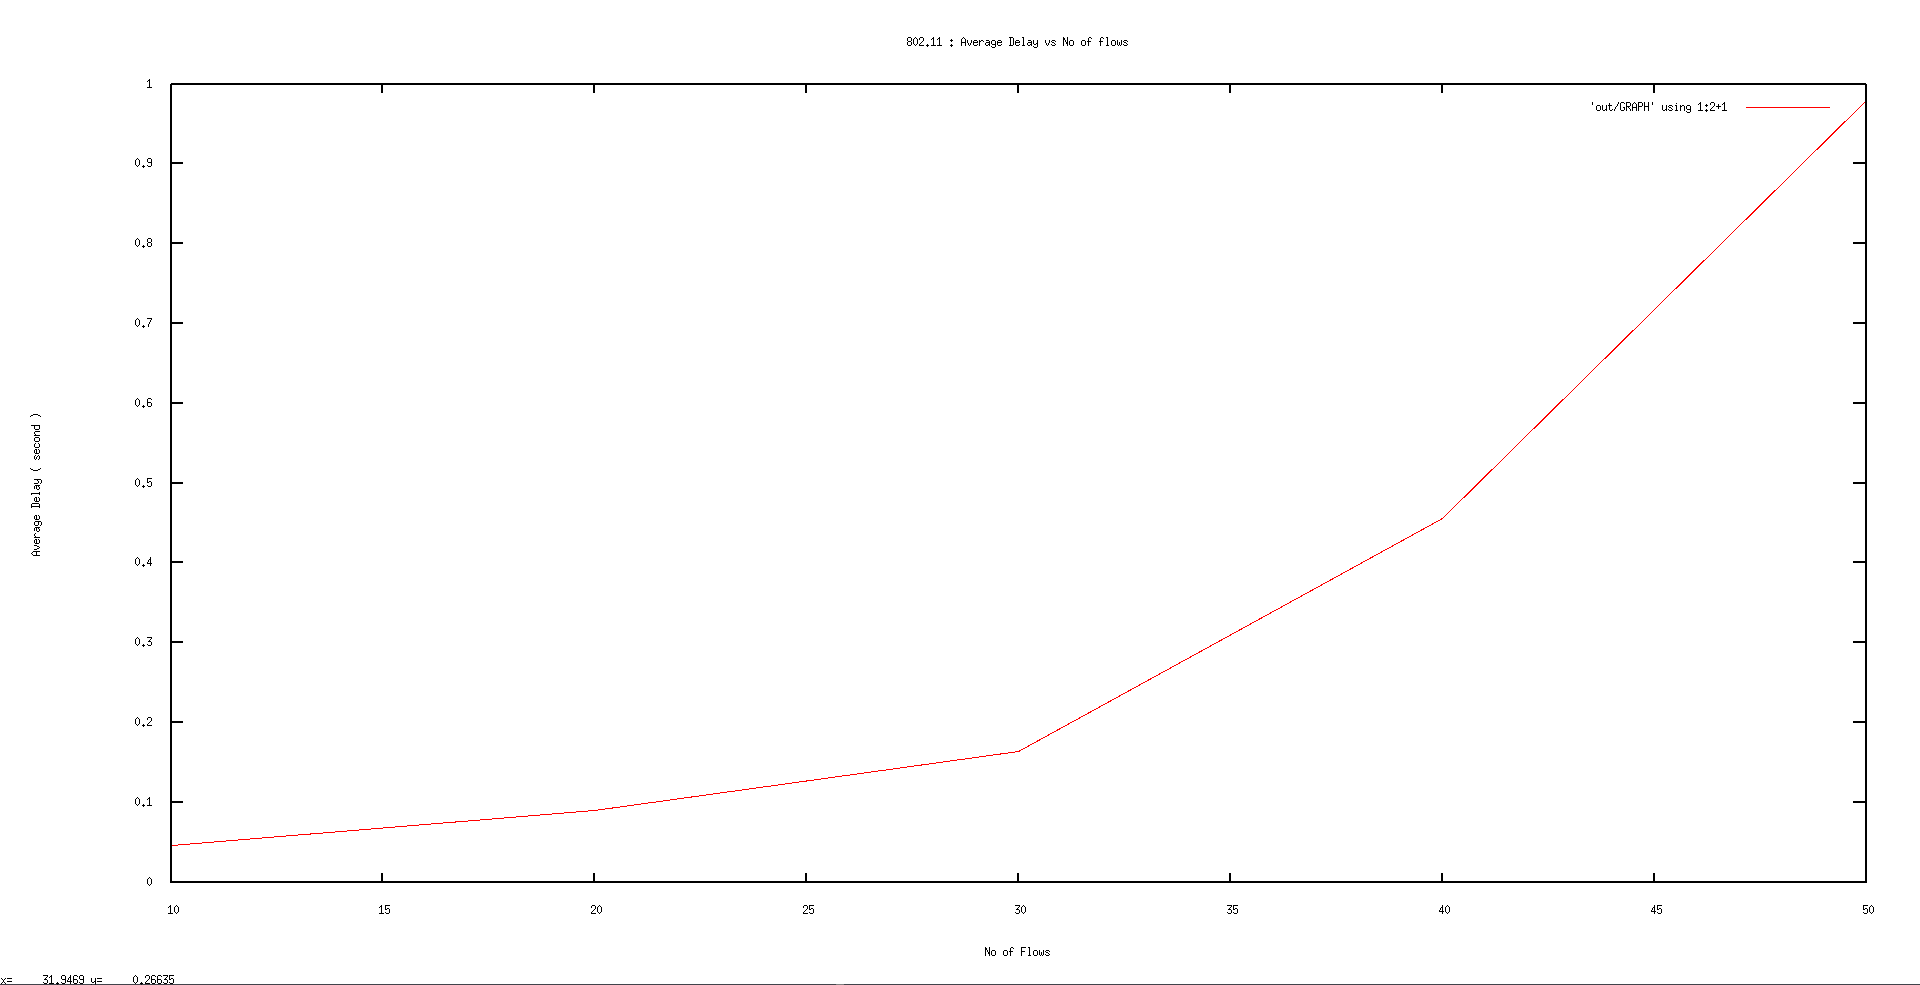
\includegraphics[scale=	0.26]{image/802.11/Averagedelay_vs_flows.png}
\end{figure}

\begin{figure}[H]
	\centering
	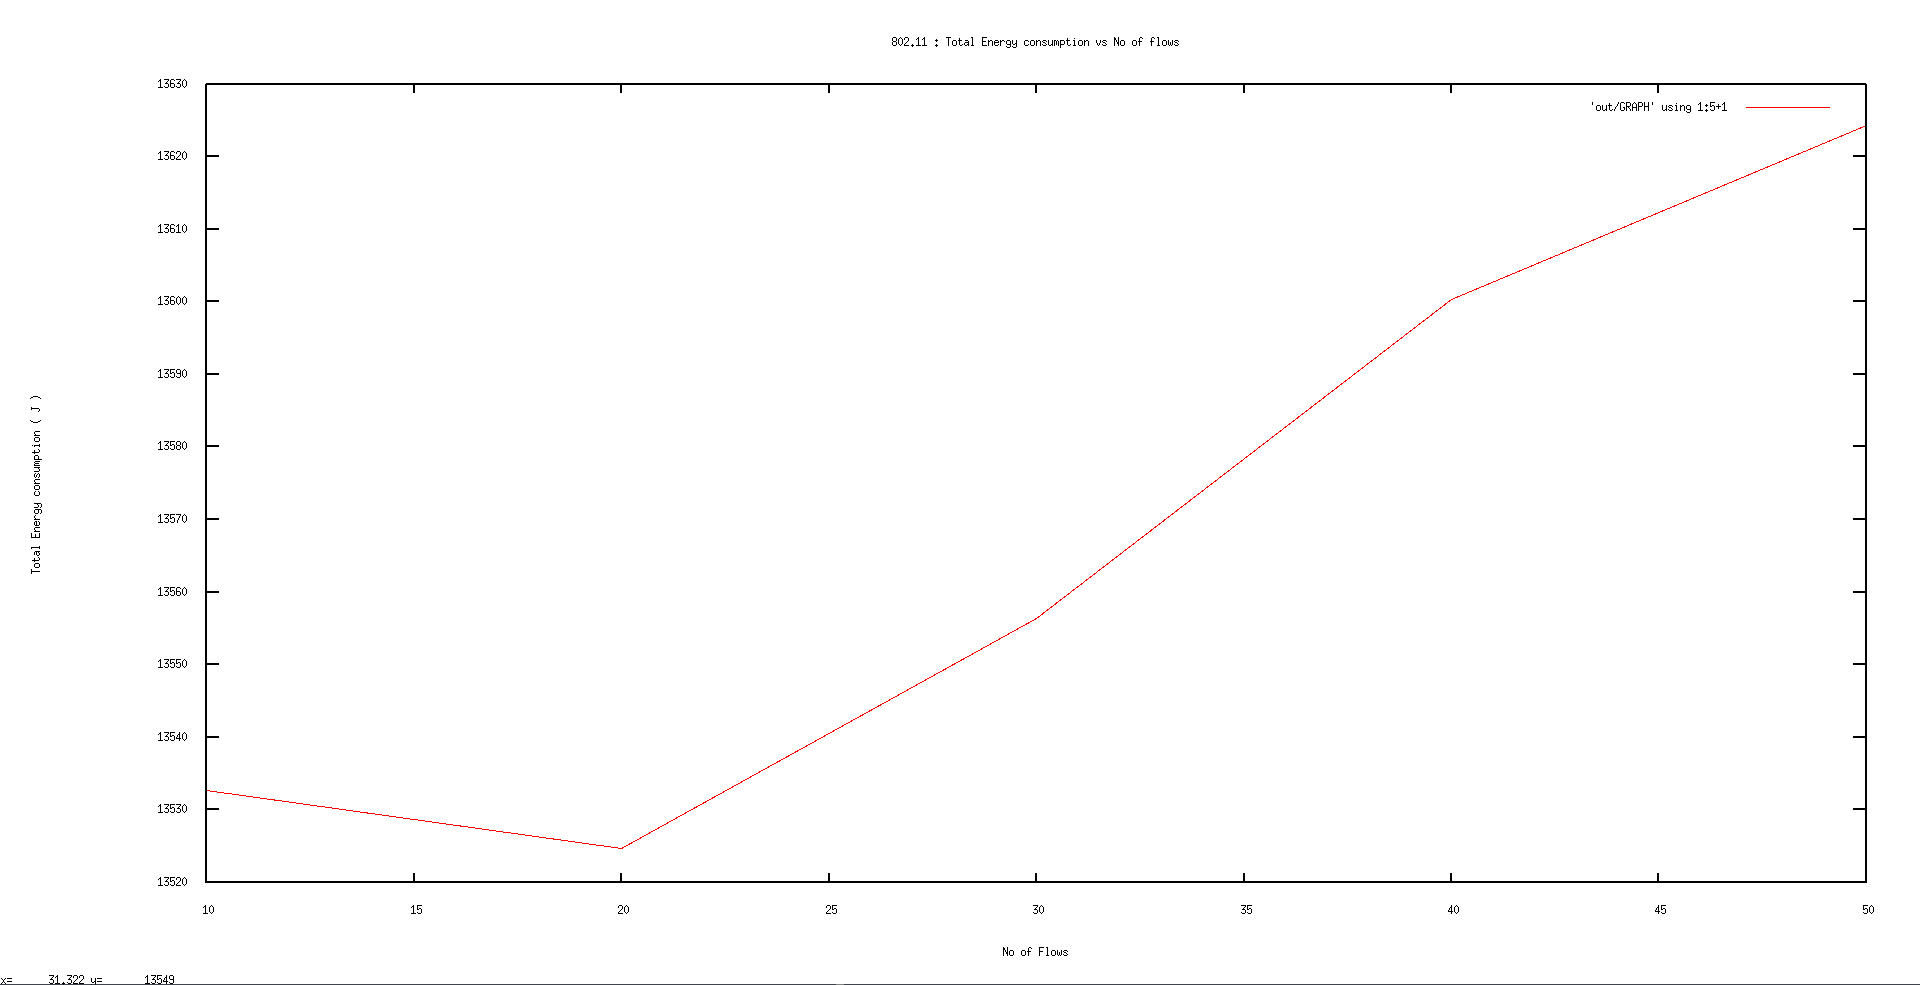
\includegraphics[scale=	0.26]{image/802.11/Energyconsumption_vs_flows.png}
\end{figure}

\begin{figure}[H]
	\centering
	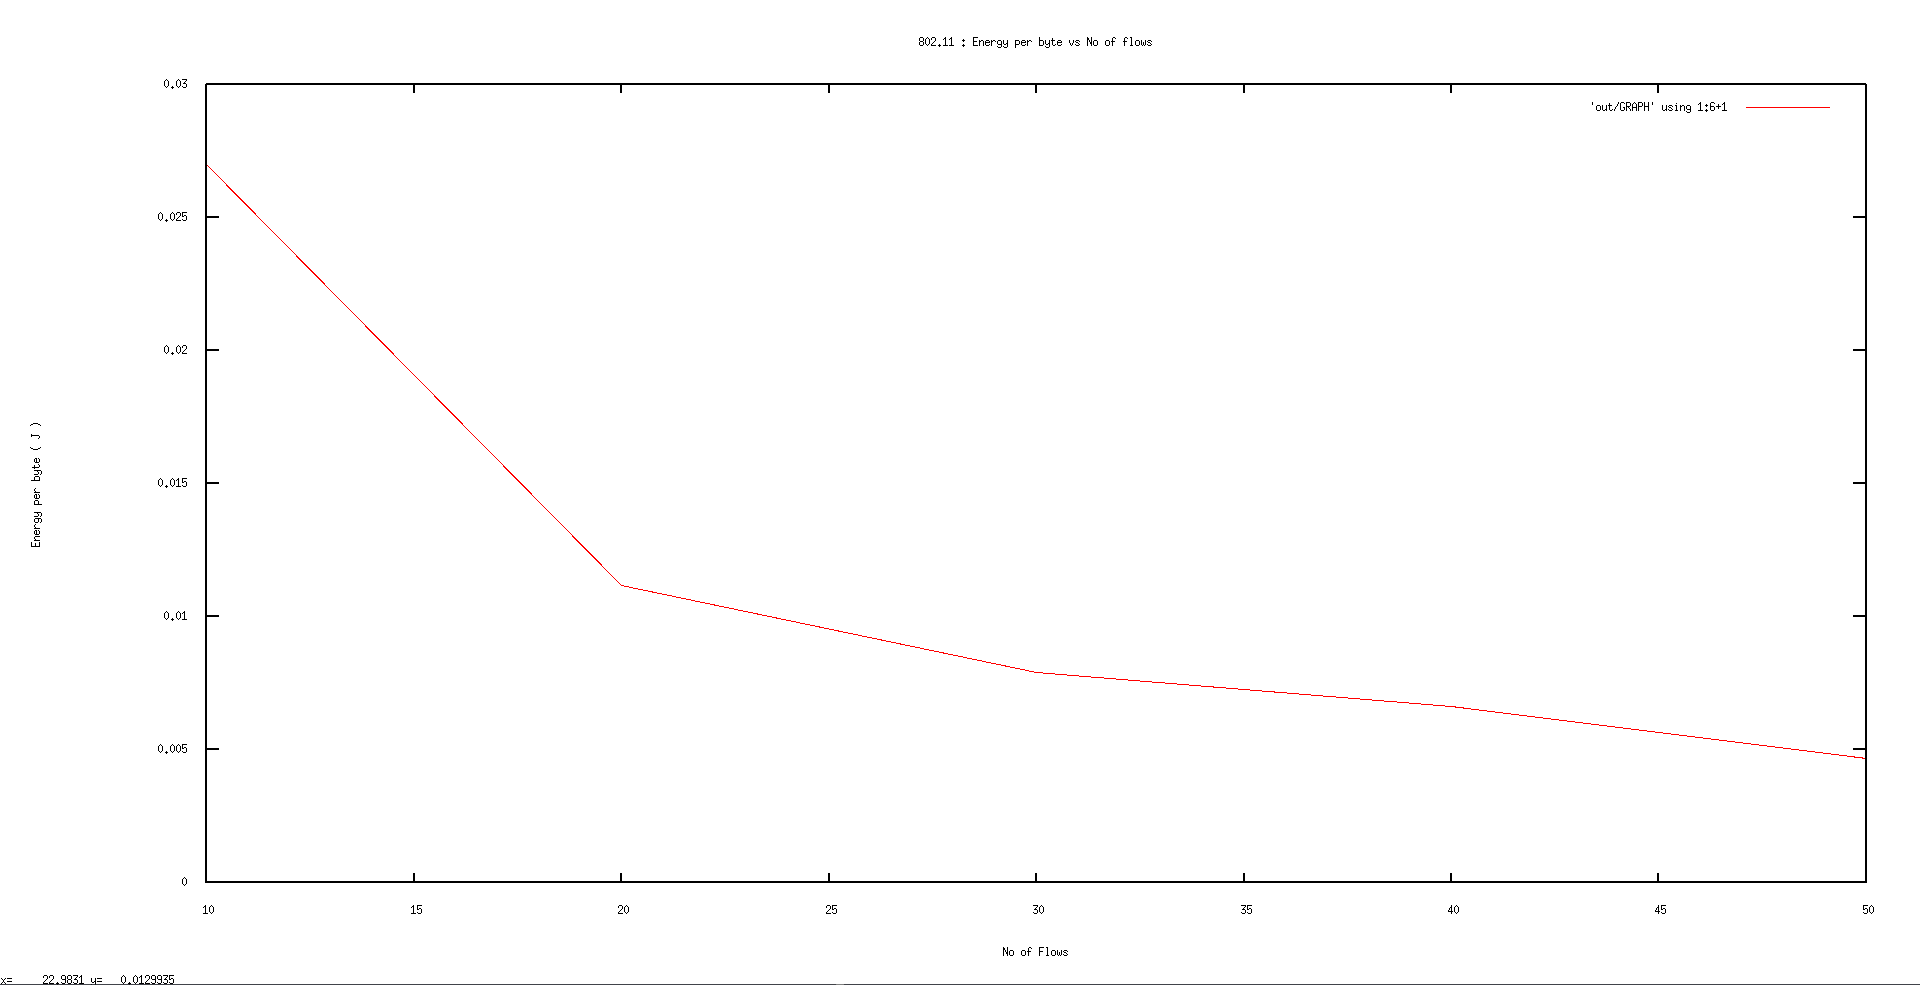
\includegraphics[scale=	0.26]{image/802.11/Energyperbytes_vs_flows.png}
\end{figure}

\begin{figure}[H]
	\centering
	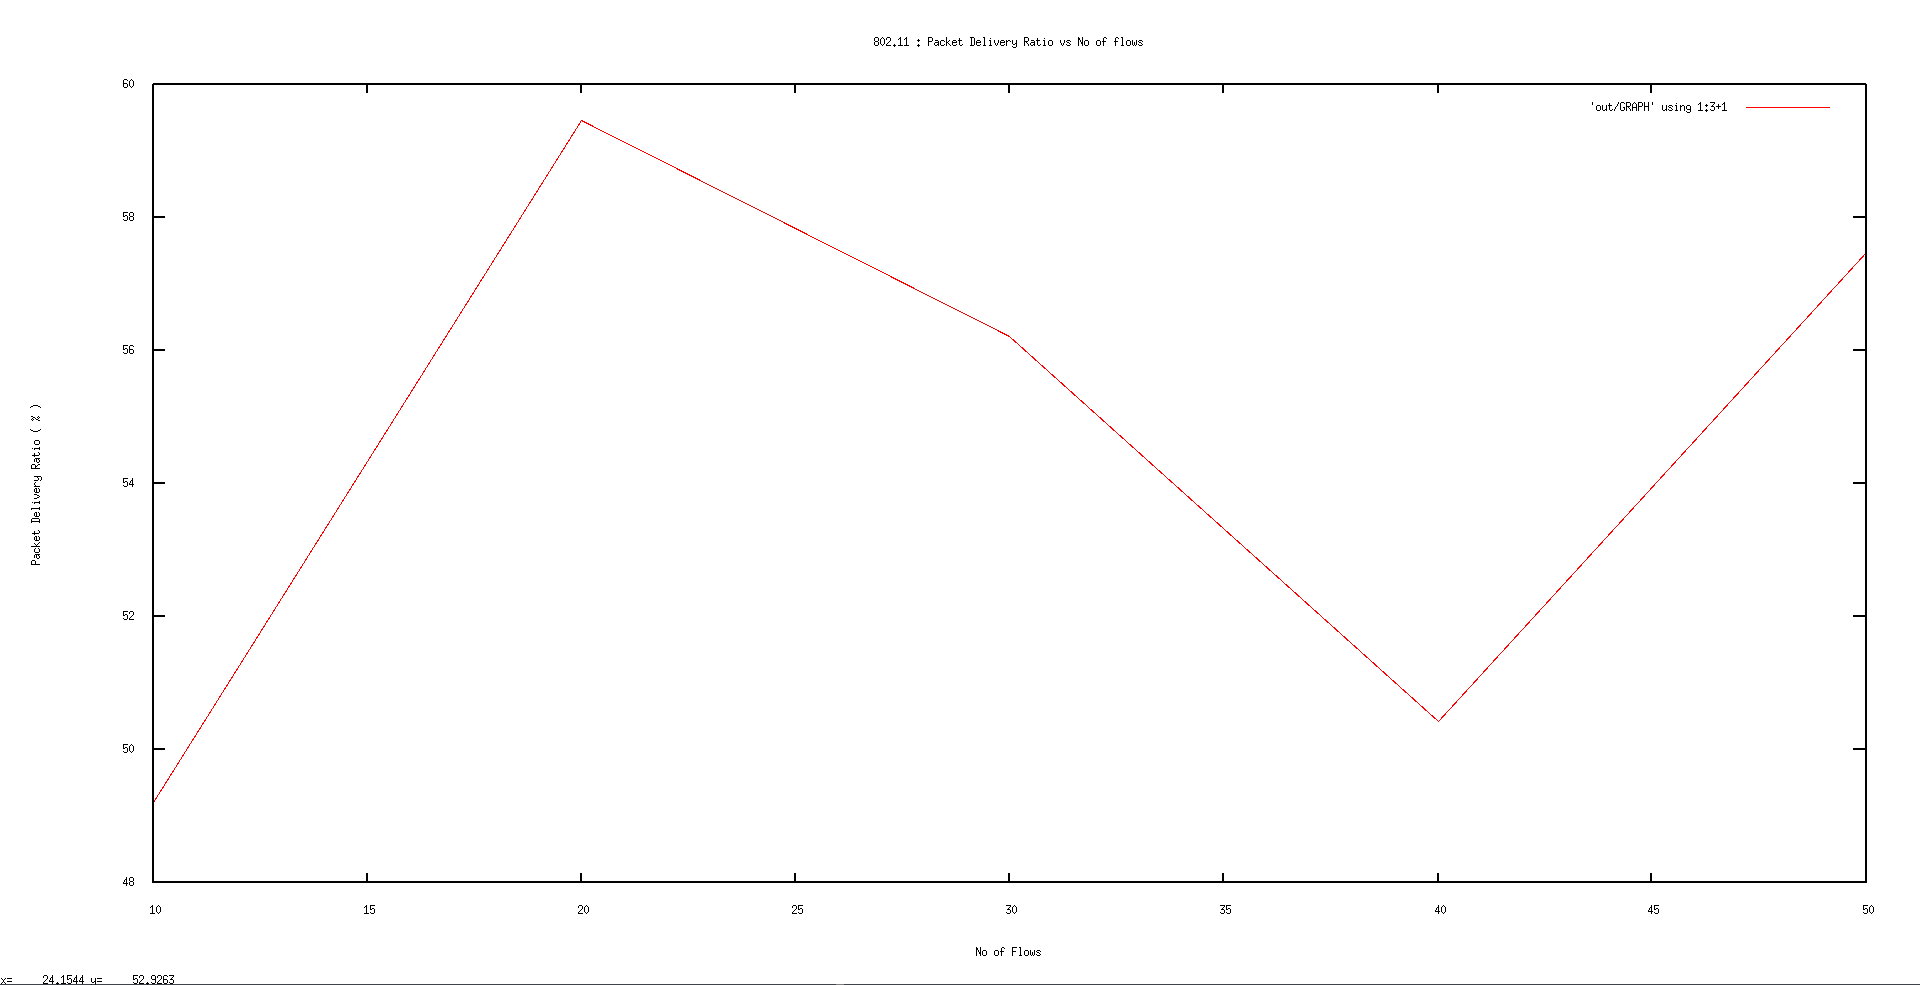
\includegraphics[scale=	0.26]{image/802.11/Packetdeliveryratio_vs_flows.png}
\end{figure}

\begin{figure}[H]
	\centering
	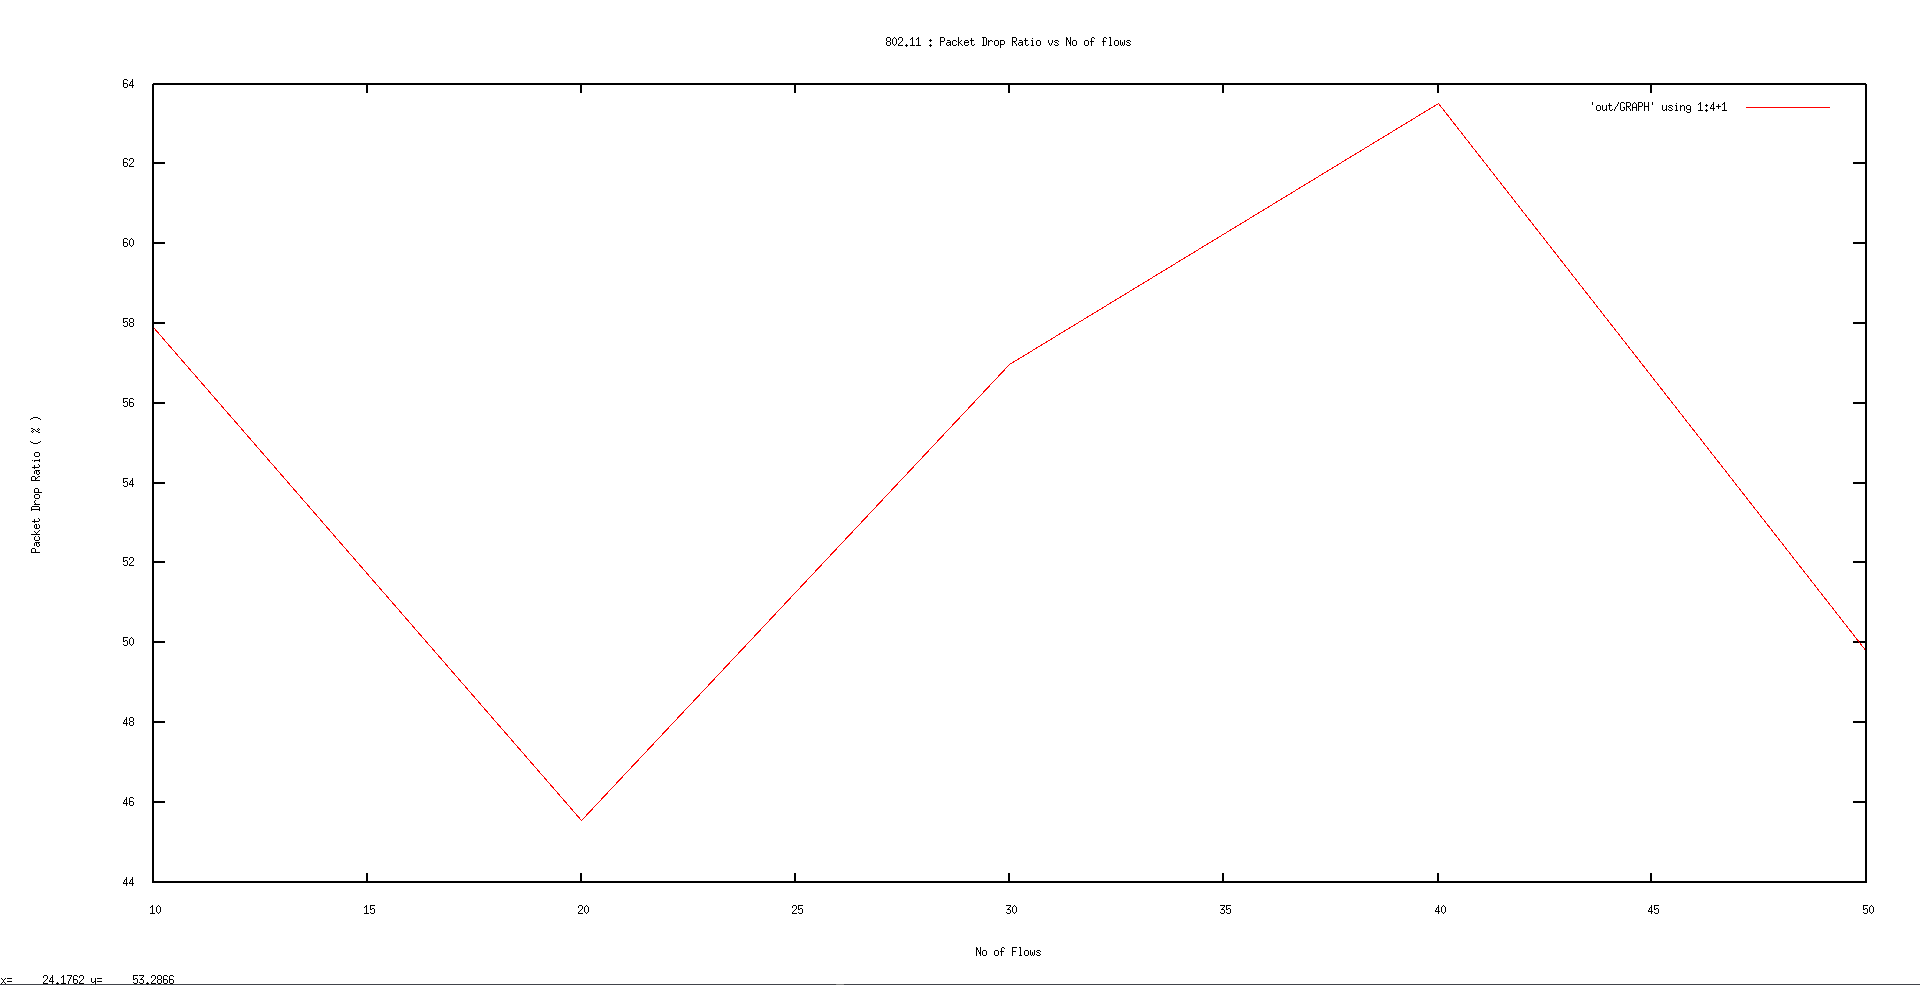
\includegraphics[scale=	0.26]{image/802.11/Packetdropratio_vs_flows.png}
\end{figure}


\newpage
\title{Variation in Packets Sent per Second}
\begin{figure}[H]
	\centering
	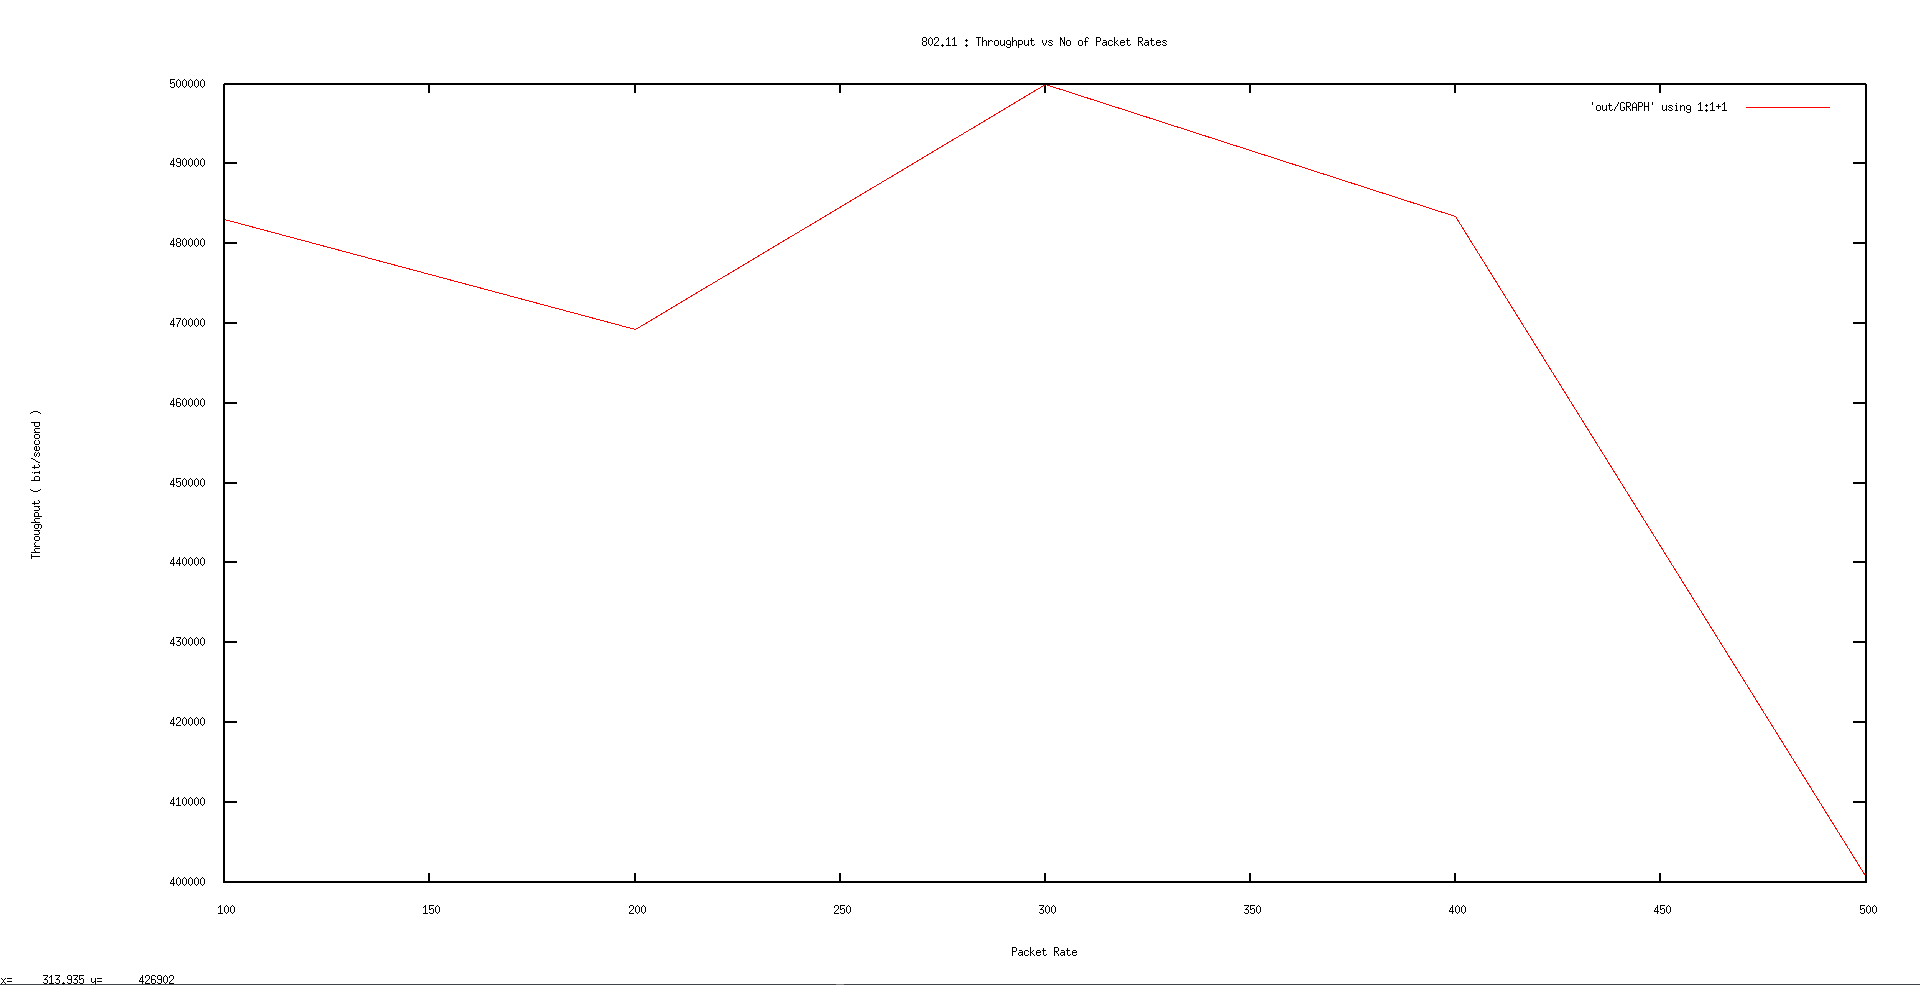
\includegraphics[scale=	0.26]{image/802.11/Throughput_vs_packetRates.png}
\end{figure}

\begin{figure}[H]
	\centering
	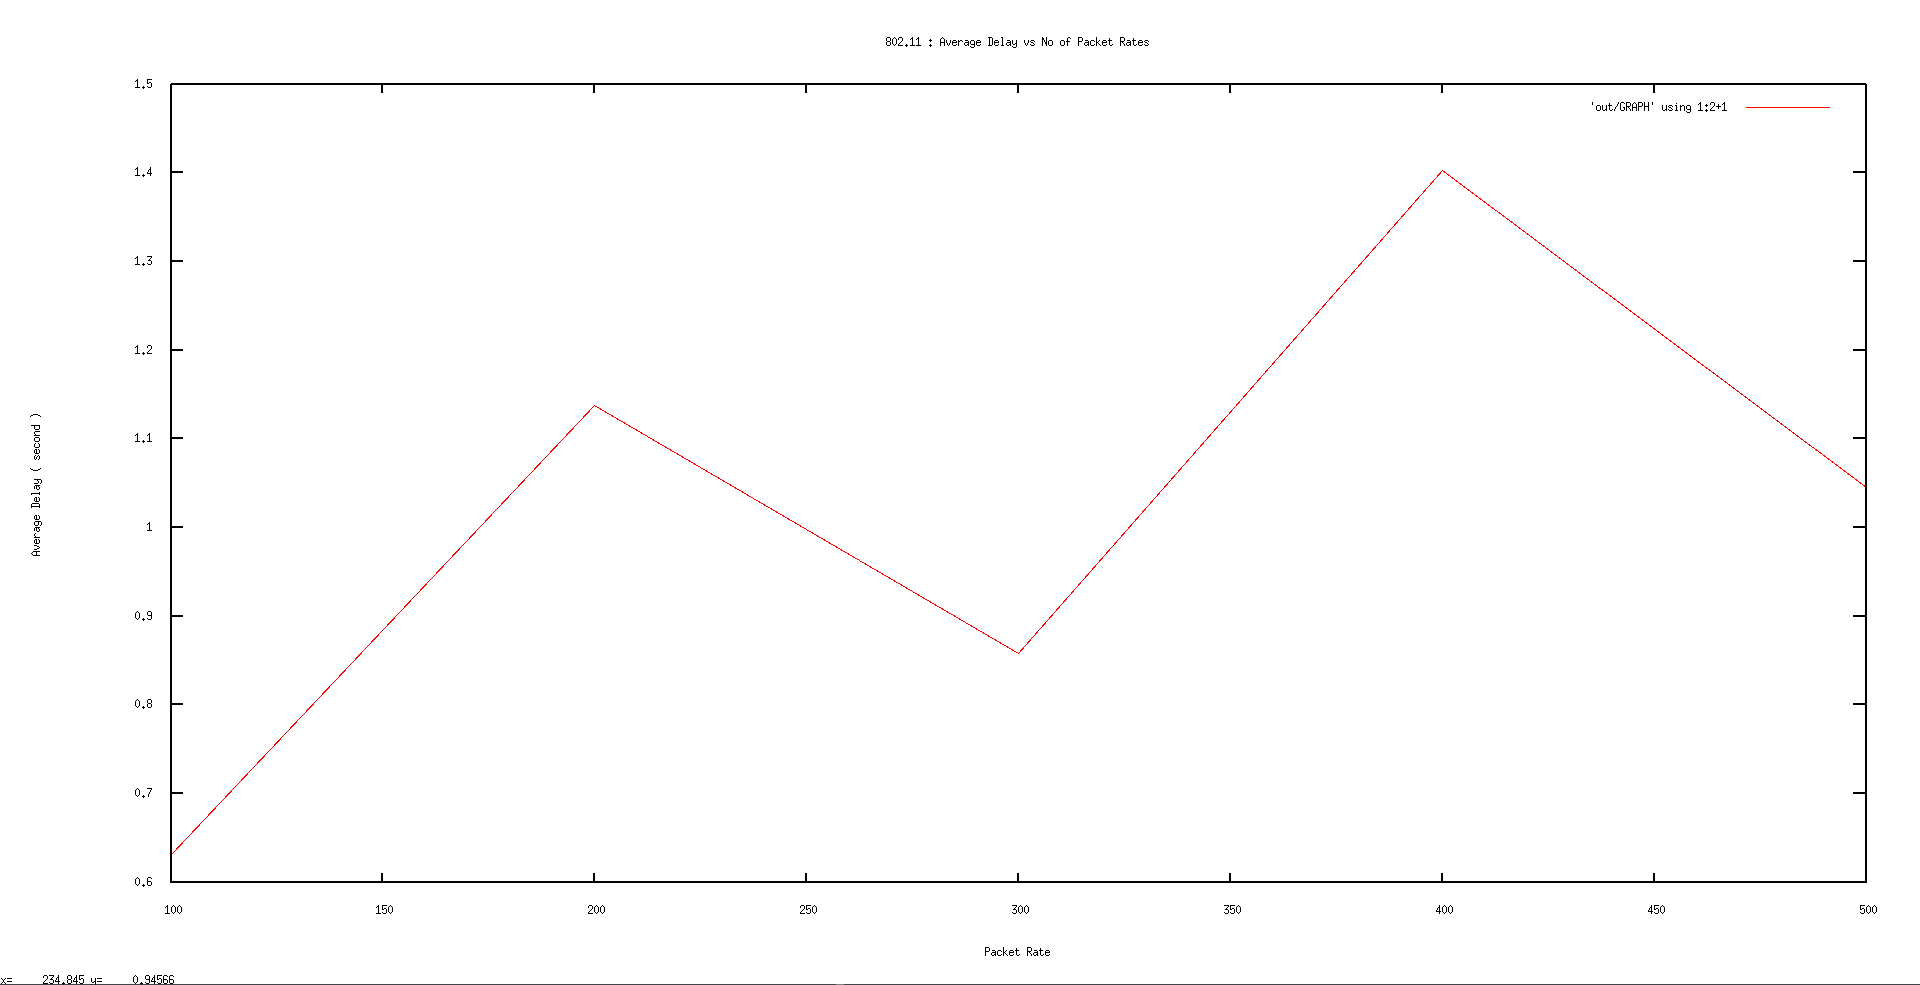
\includegraphics[scale=	0.26]{image/802.11/Averagedelay_vs_packetRates.png}
\end{figure}

\begin{figure}[H]
	\centering
	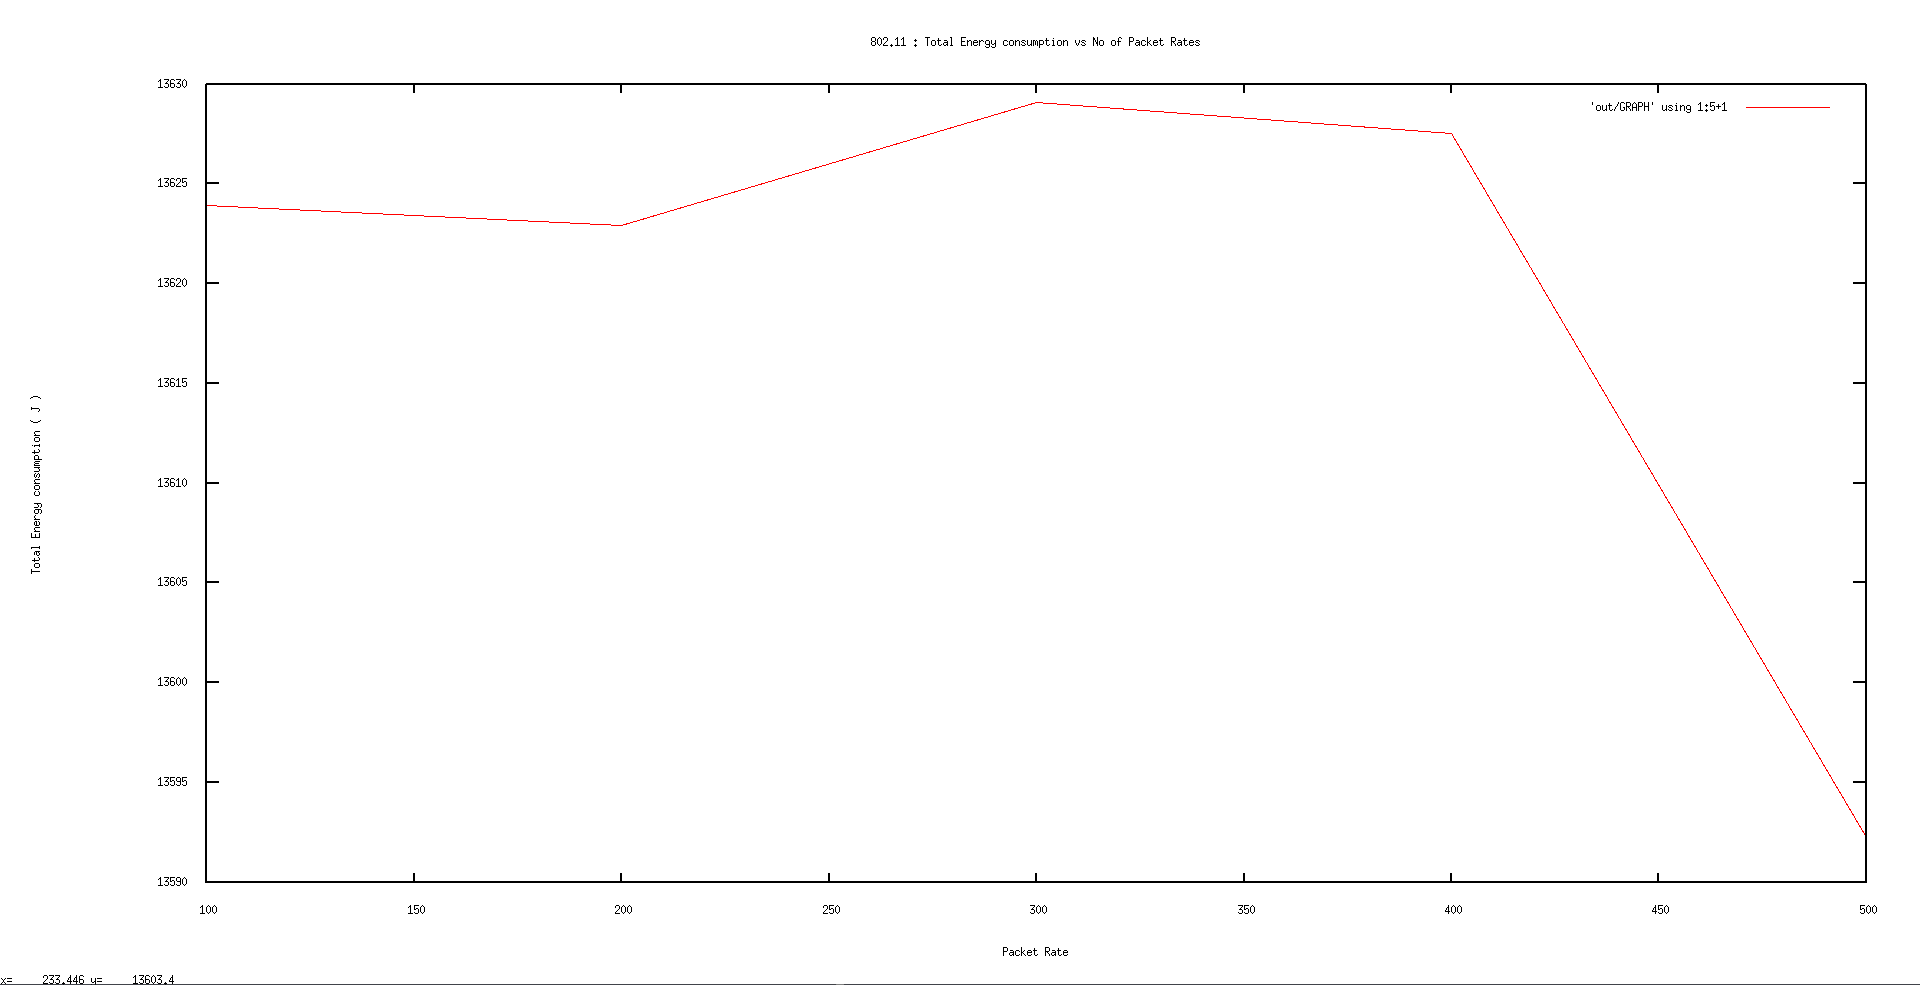
\includegraphics[scale=	0.26]{image/802.11/Energyconsumption_vs_packetRates.png}
\end{figure}

\begin{figure}[H]
	\centering
	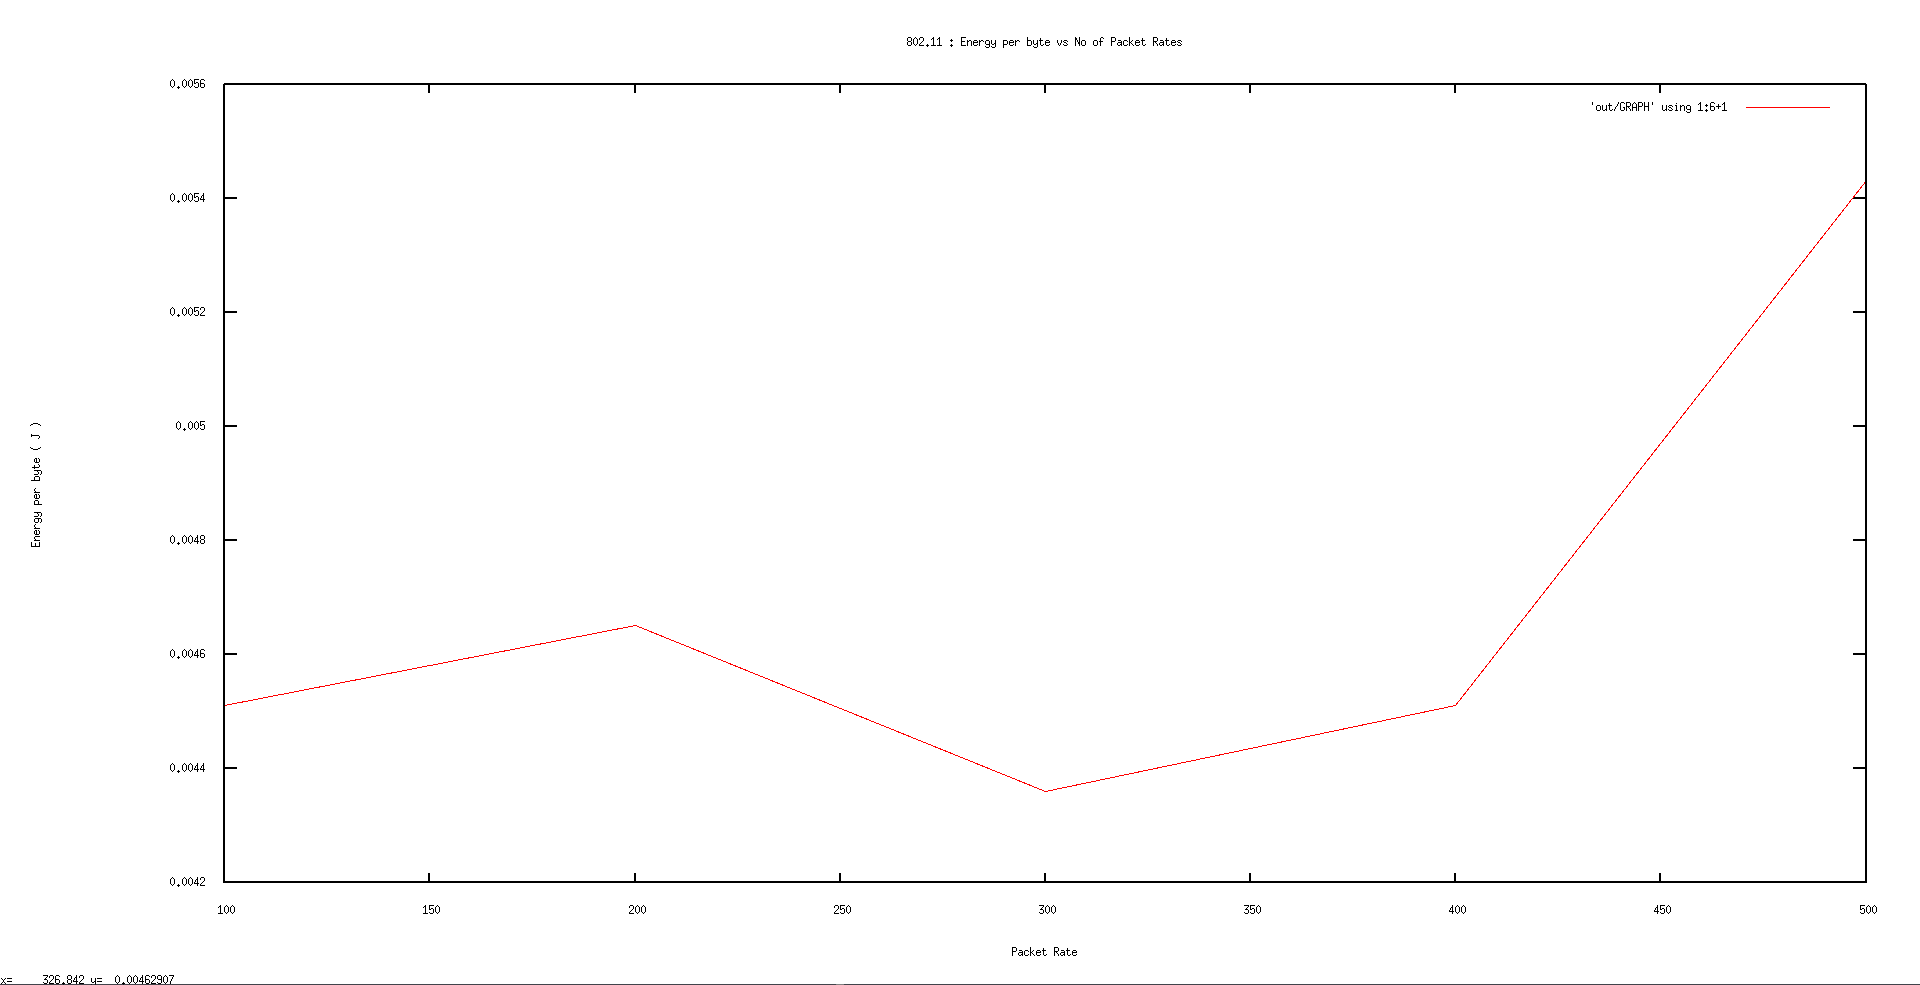
\includegraphics[scale=	0.26]{image/802.11/Energyperbytes_vs_packetRates.png}
\end{figure}

\begin{figure}[H]
	\centering
	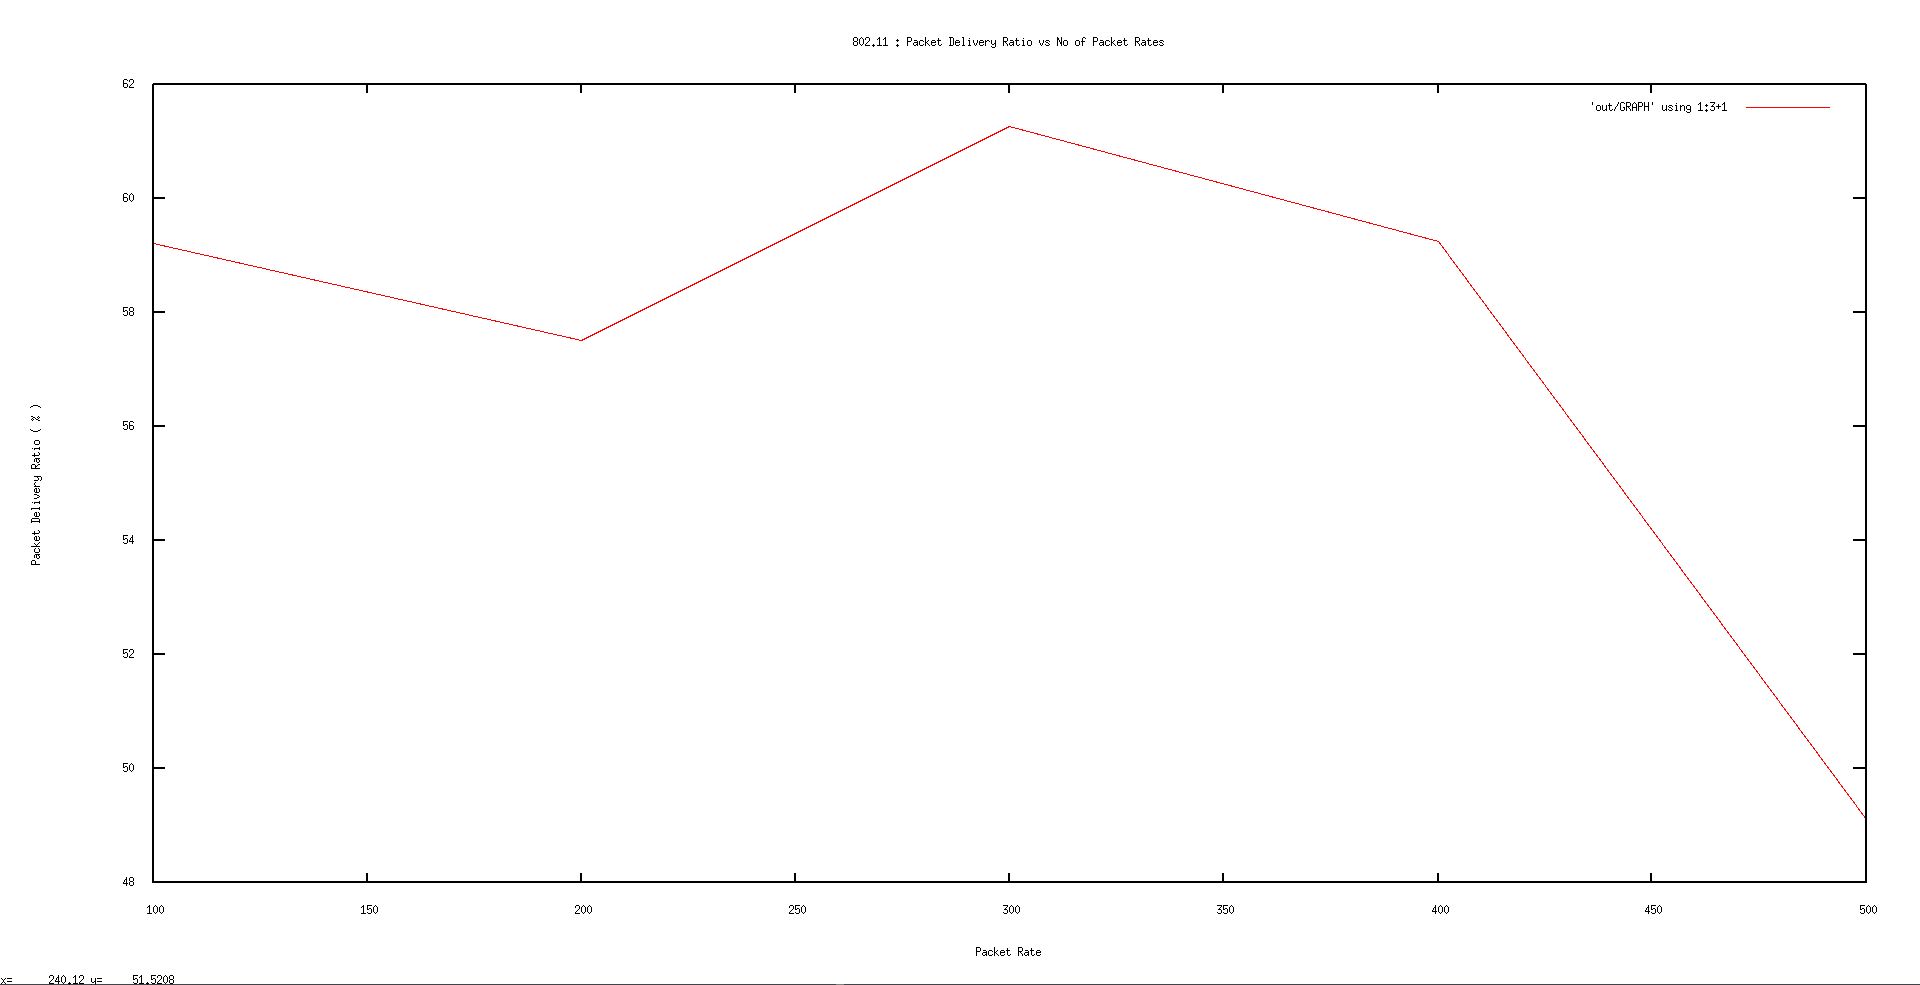
\includegraphics[scale=	0.26]{image/802.11/Packetdeliveryratio_vs_packetRates.png}
\end{figure}

\begin{figure}[H]
	\centering
	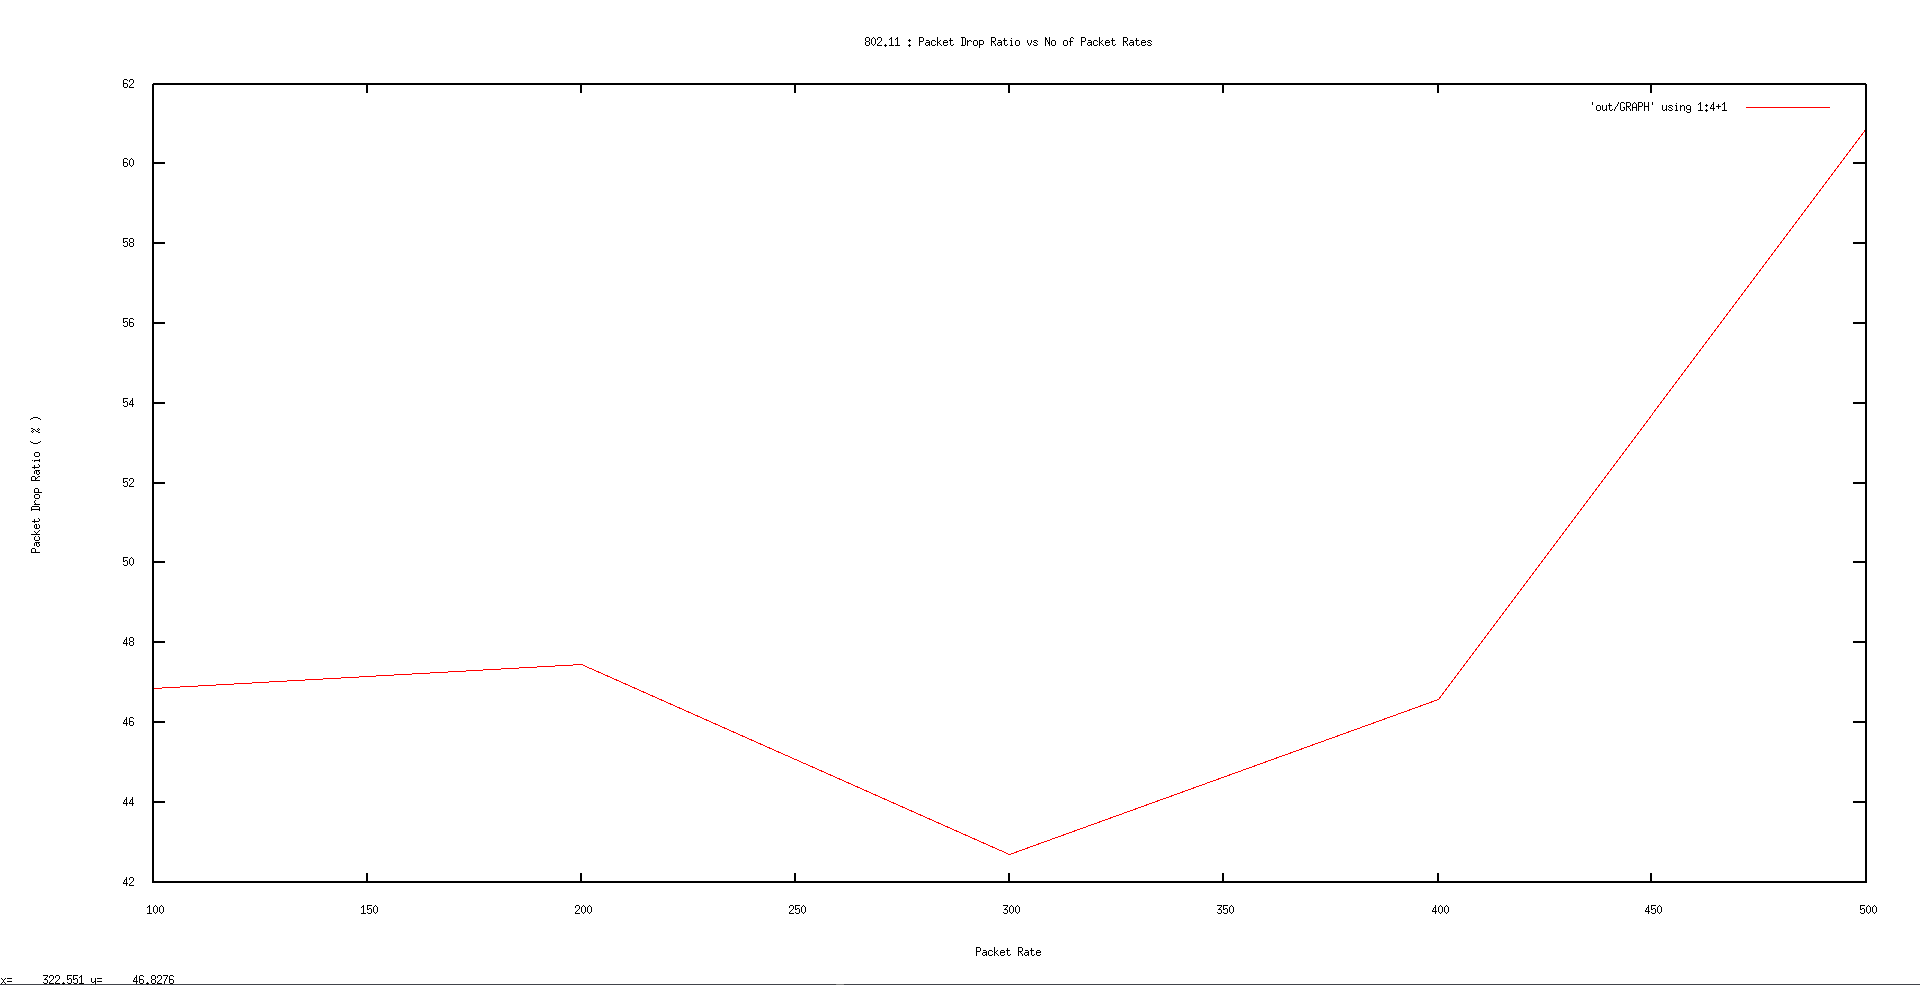
\includegraphics[scale=	0.26]{image/802.11/Packetdropratio_vs_packetRates.png}
\end{figure}

\newpage
\title{Variation in Speed}
\begin{figure}[H]
	\centering
	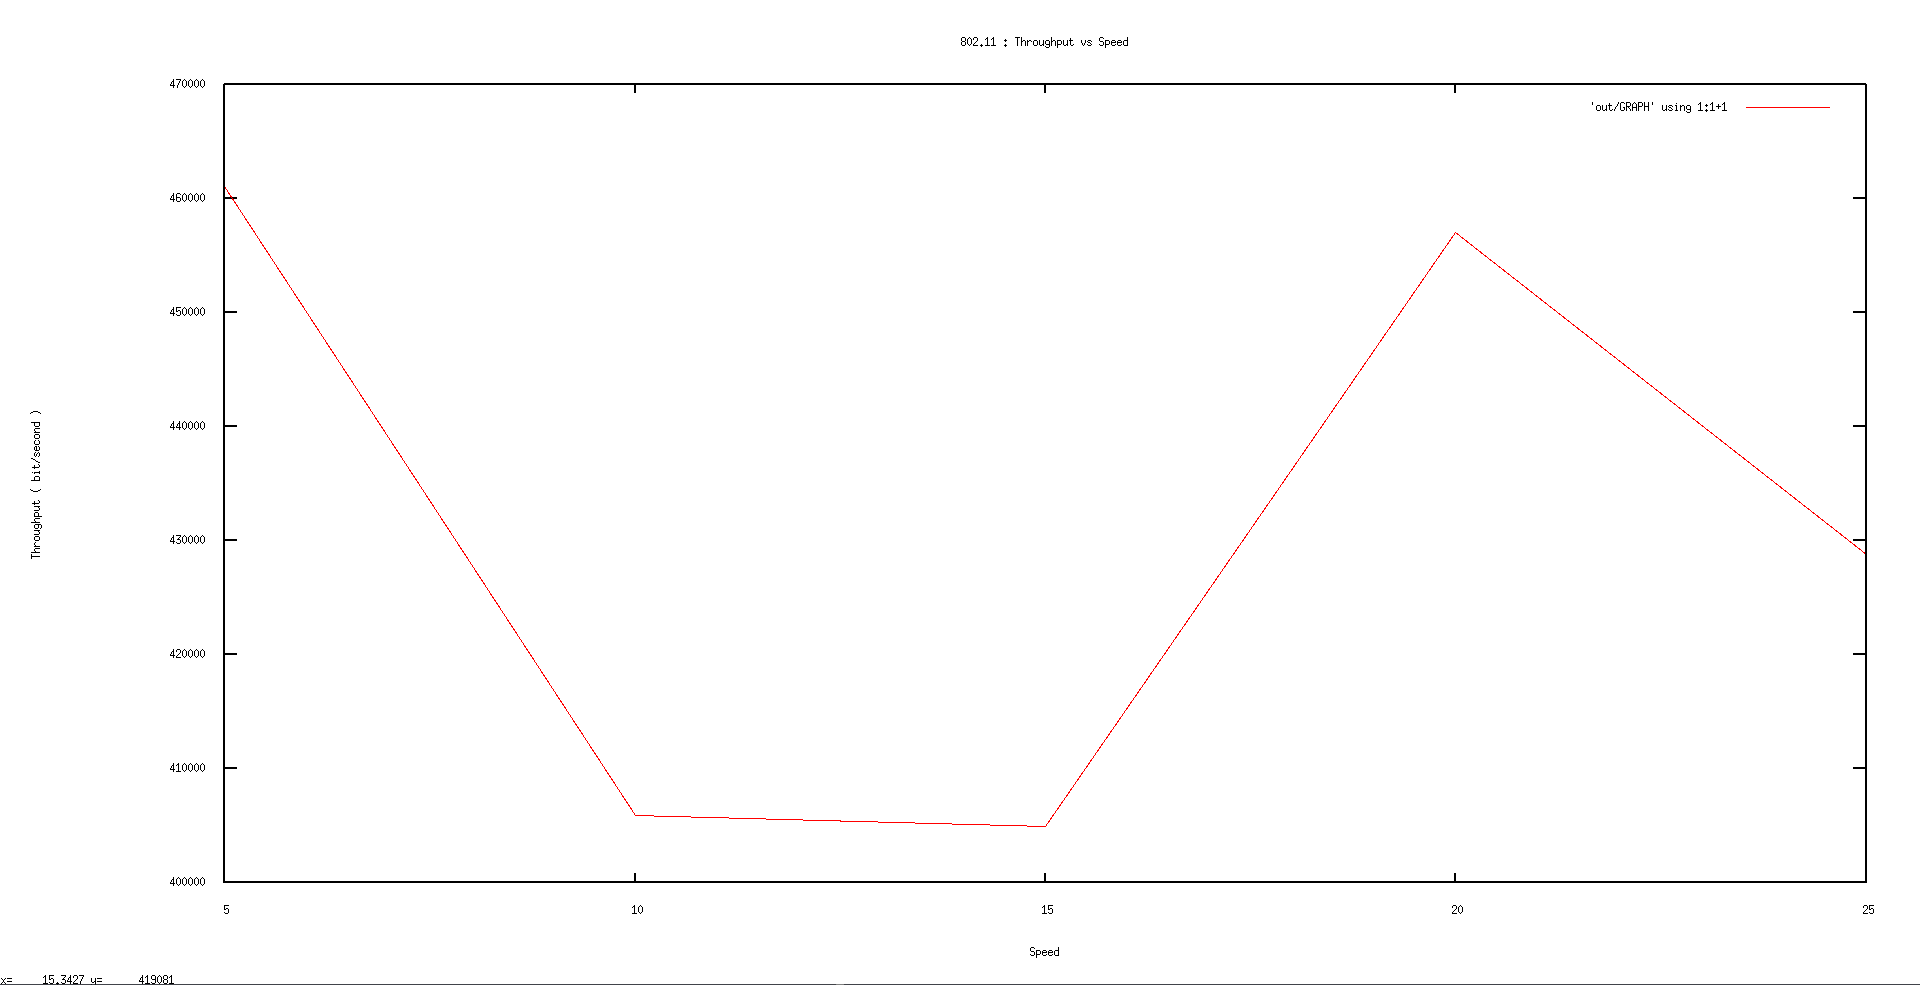
\includegraphics[scale=	0.26]{image/802.11/Throughput_vs_speed.png}
\end{figure}

\begin{figure}[H]
	\centering
	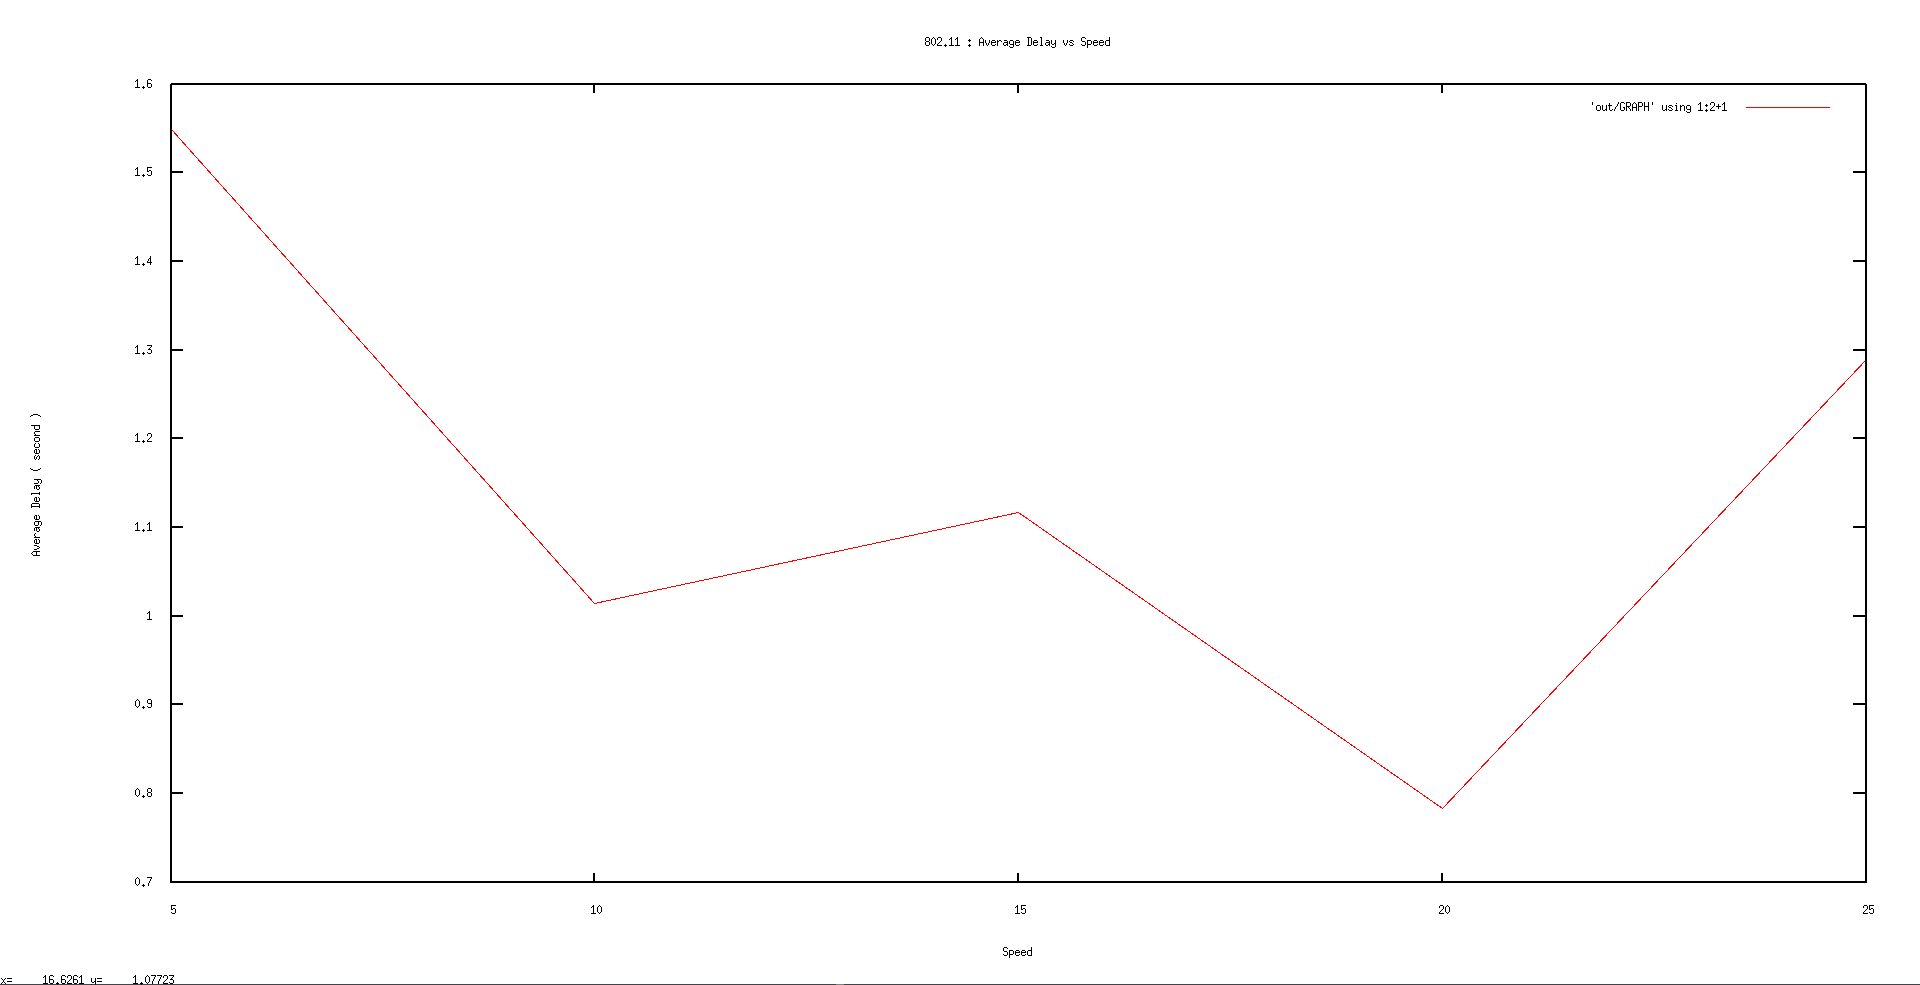
\includegraphics[scale=	0.26]{image/802.11/Averagedelay_vs_speed.png}
\end{figure}

\begin{figure}[H]
	\centering
	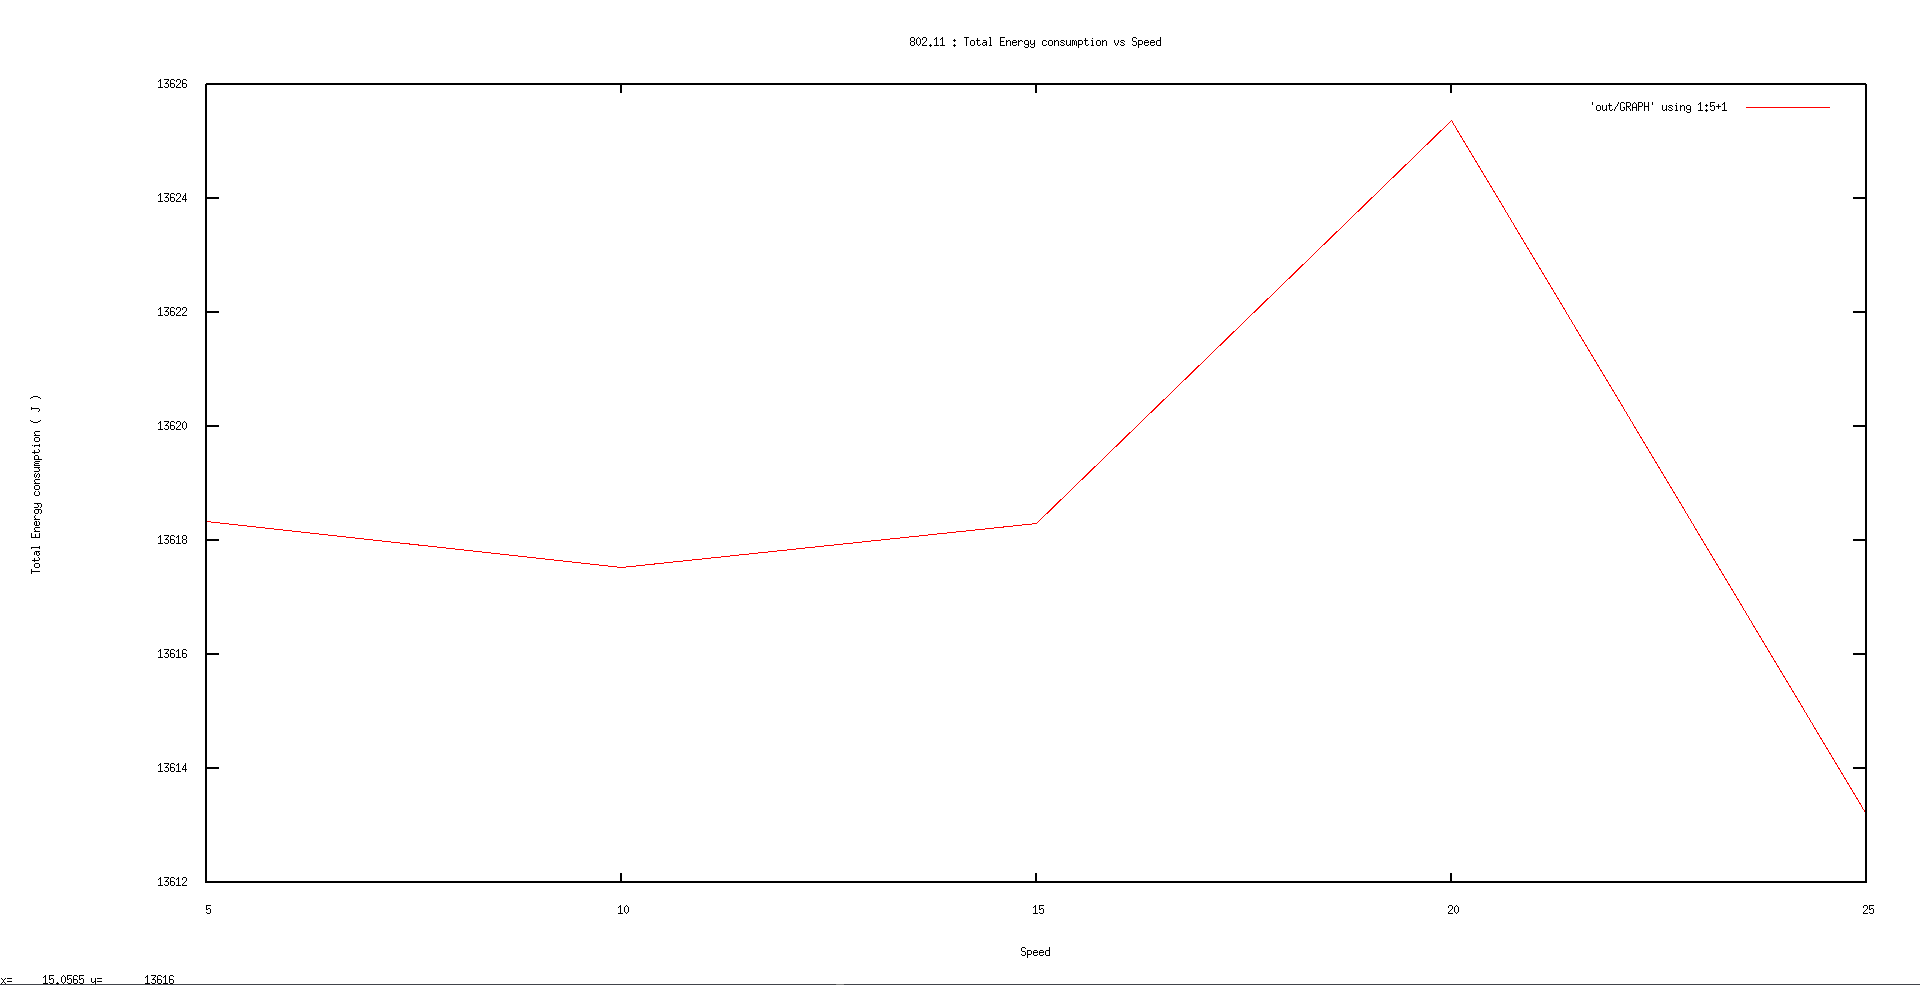
\includegraphics[scale=	0.26]{image/802.11/Energyconsumption_vs_speed.png}
\end{figure}

\begin{figure}[H]
	\centering
	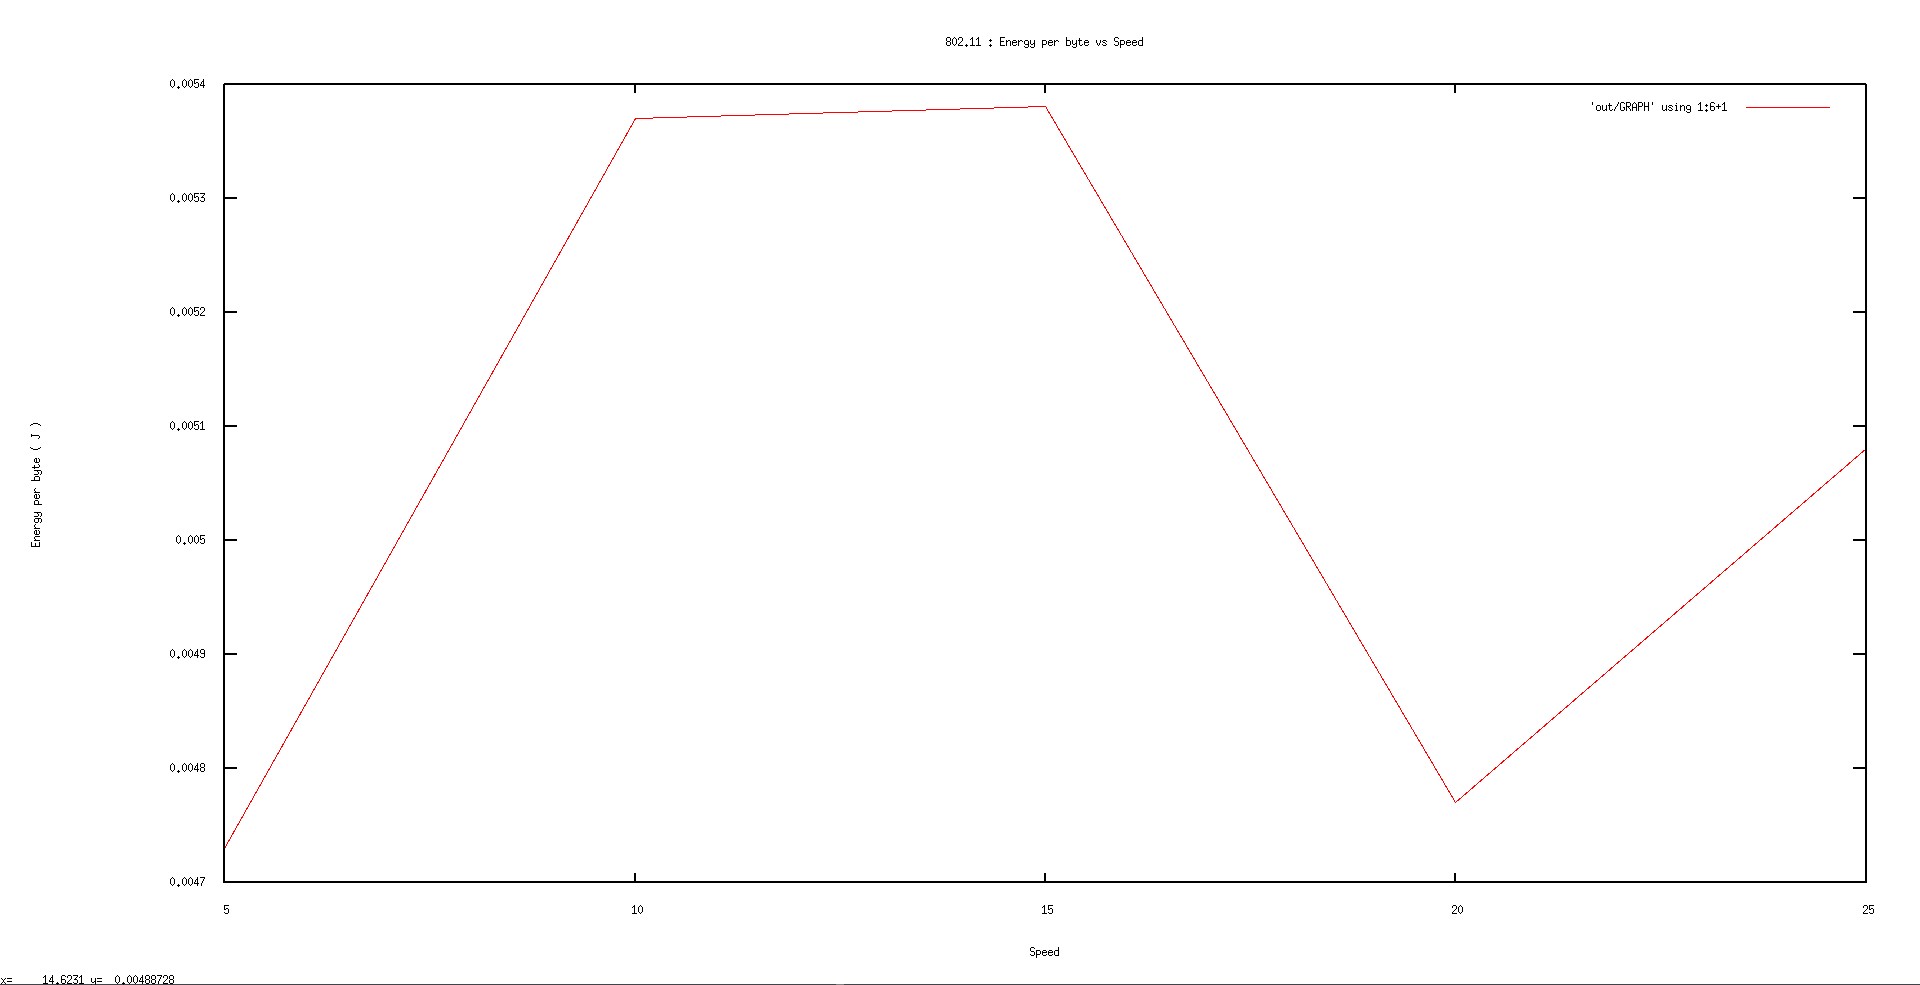
\includegraphics[scale=	0.26]{image/802.11/Energyperbytes_vs_speed.png}
\end{figure}

\begin{figure}[H]
	\centering
	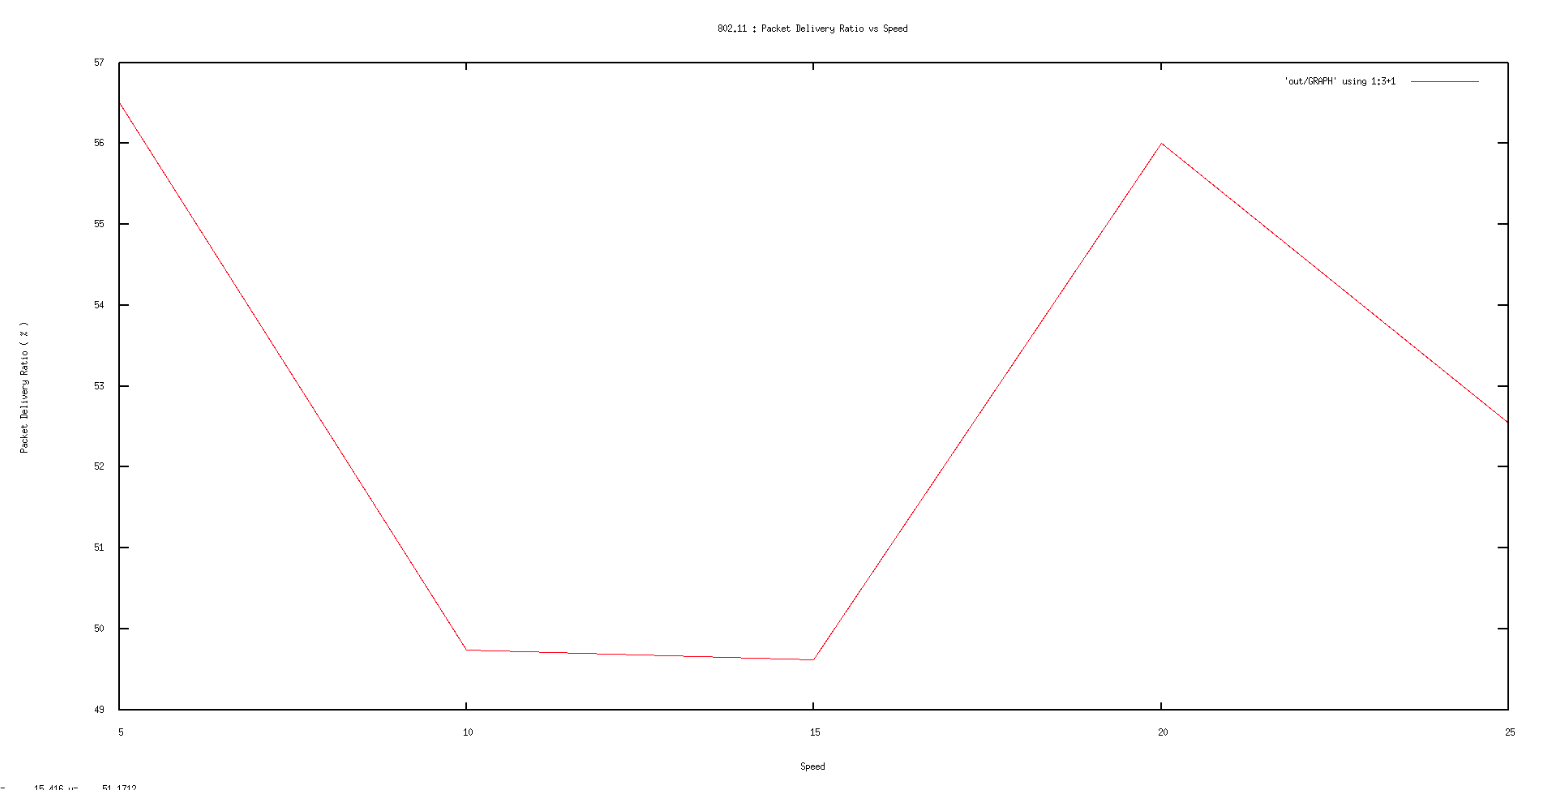
\includegraphics[scale=	0.26]{image/802.11/Packetdeliveryratio_vs_speed.png}
\end{figure}

\begin{figure}[H]
	\centering
	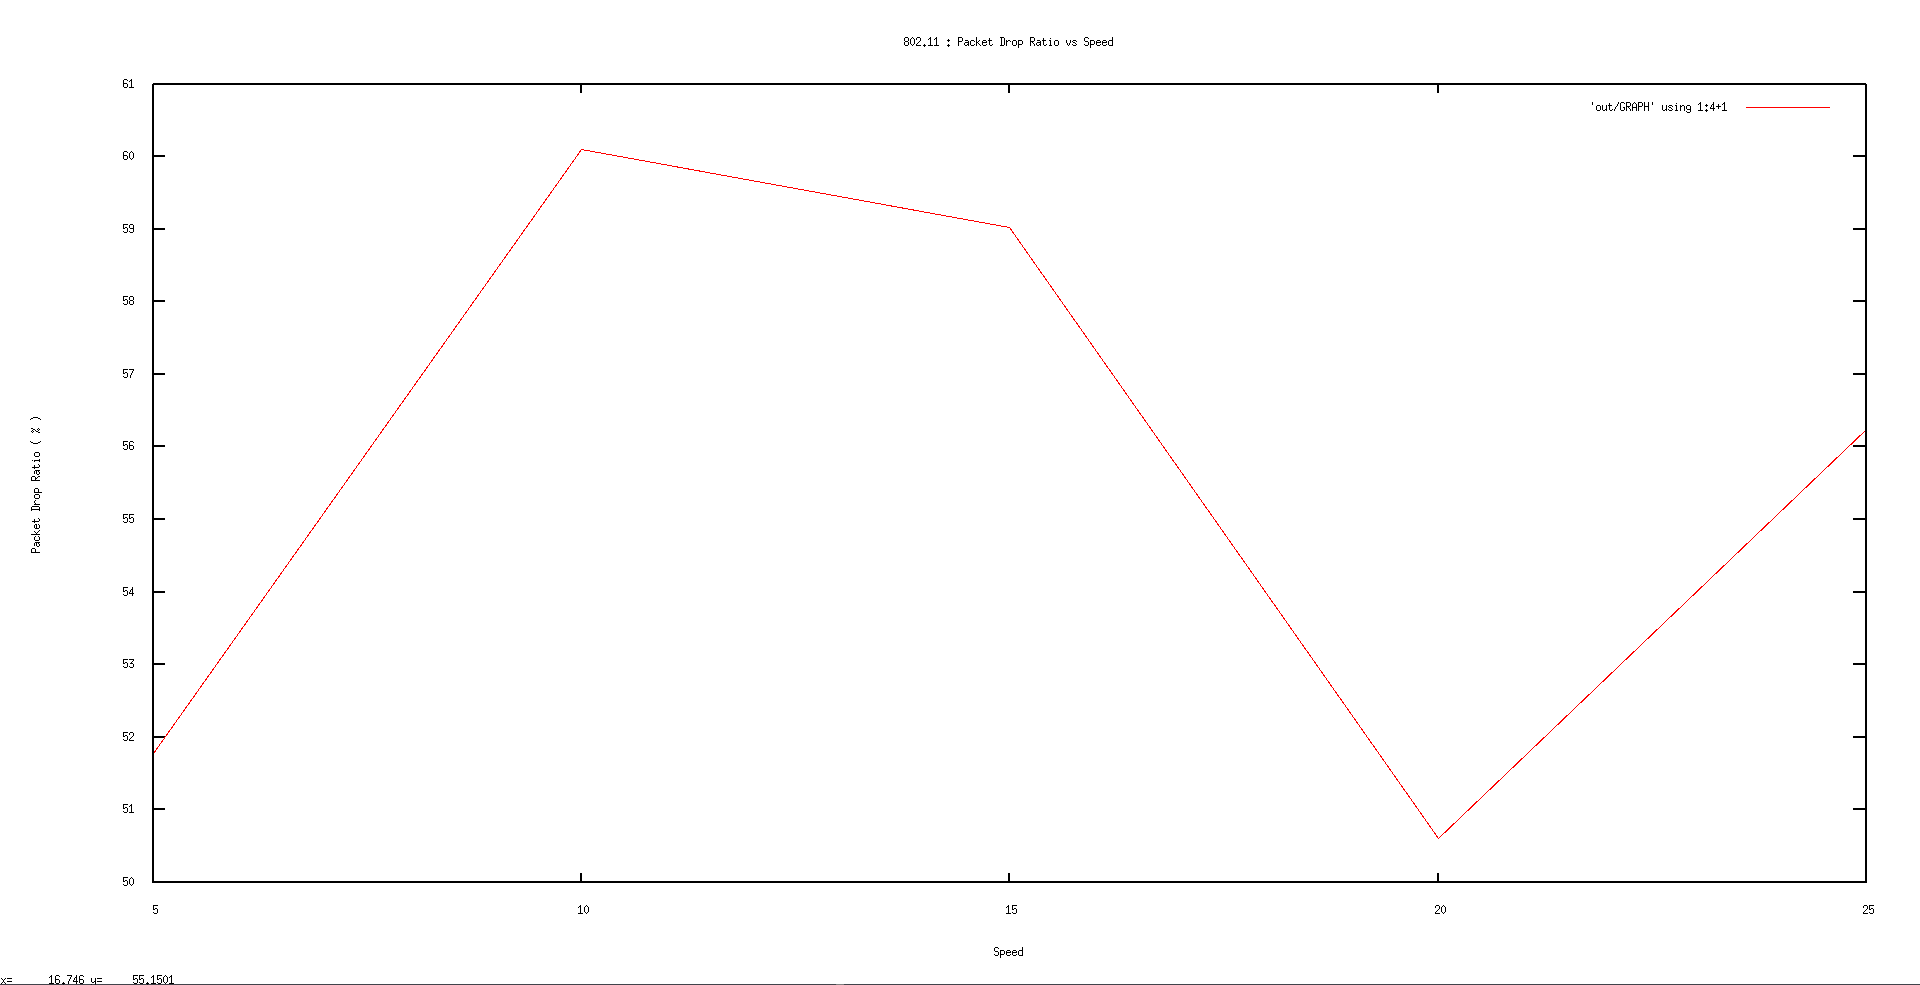
\includegraphics[scale=	0.26]{image/802.11/Packetdropratio_vs_speed.png}
\end{figure}




\newpage
\subsection{802.15.4}

\title{Variation in Number of Nodes}
\begin{figure}[H]
	\centering
	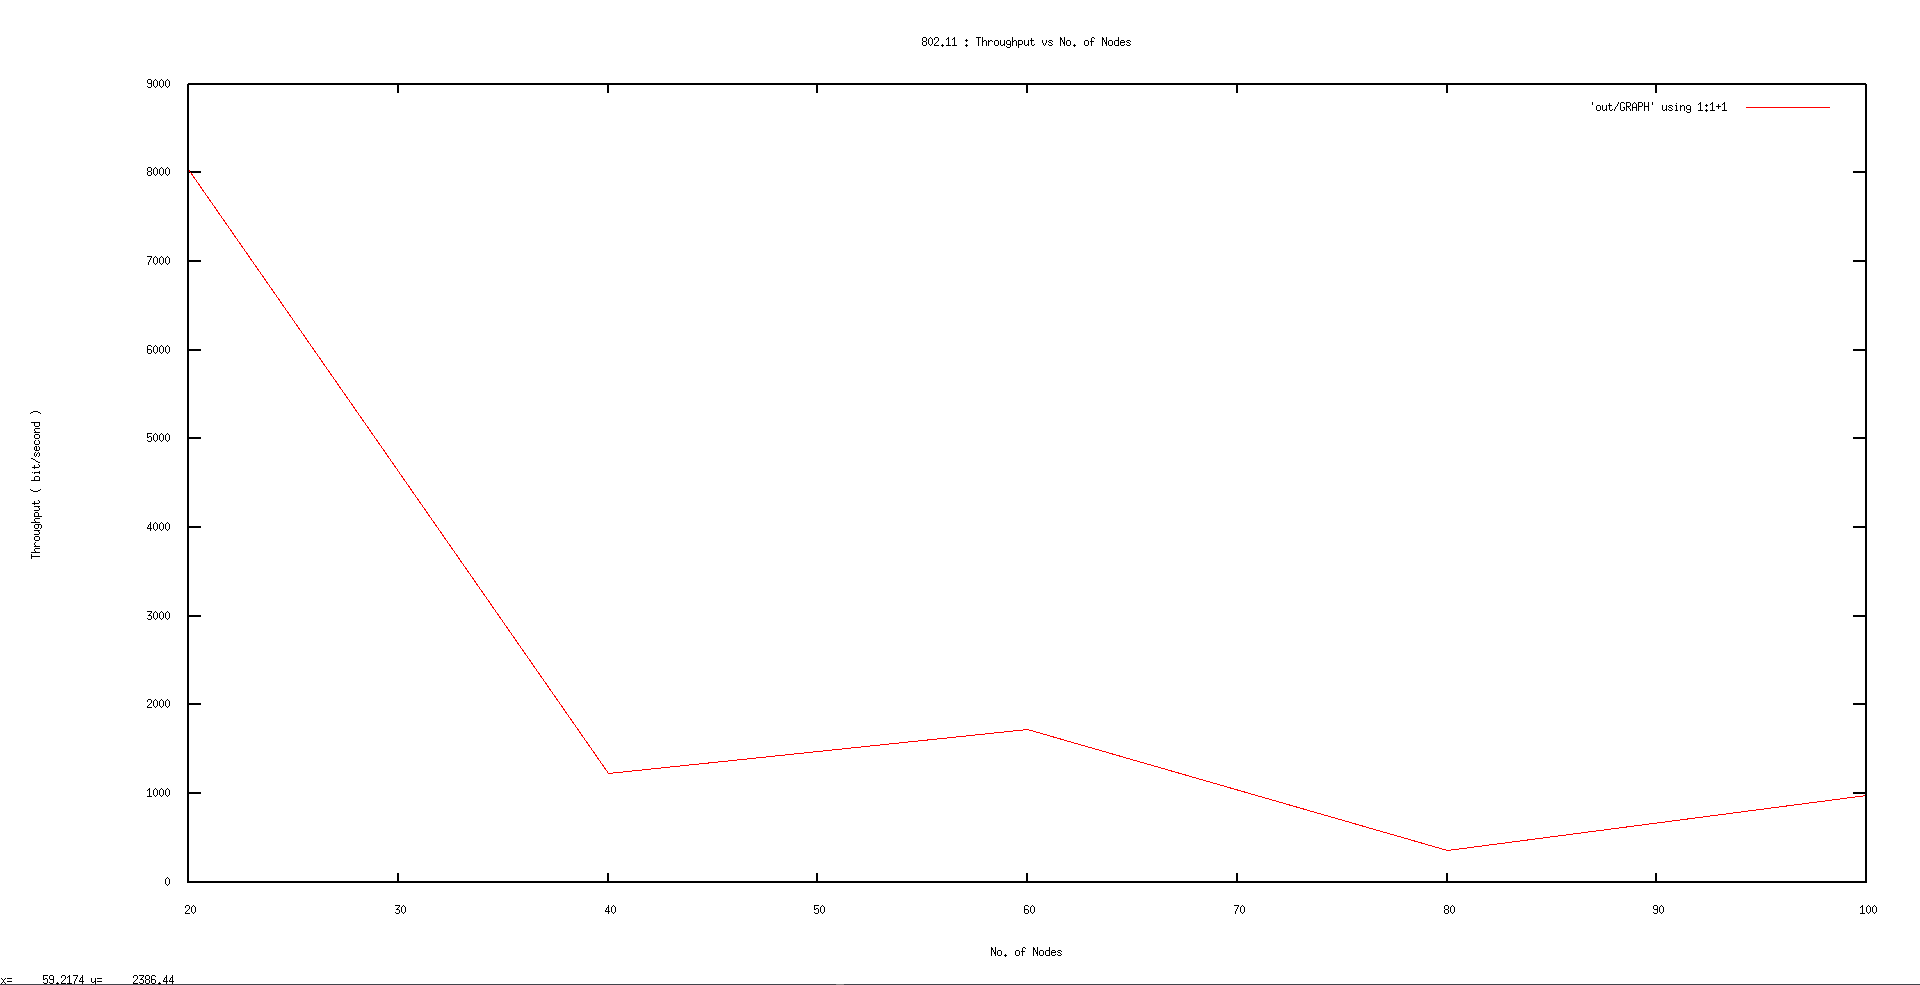
\includegraphics[scale=	0.26]{image/802.15.4/Throughput_vs_nodes.png}
\end{figure}

\begin{figure}[H]
	\centering
	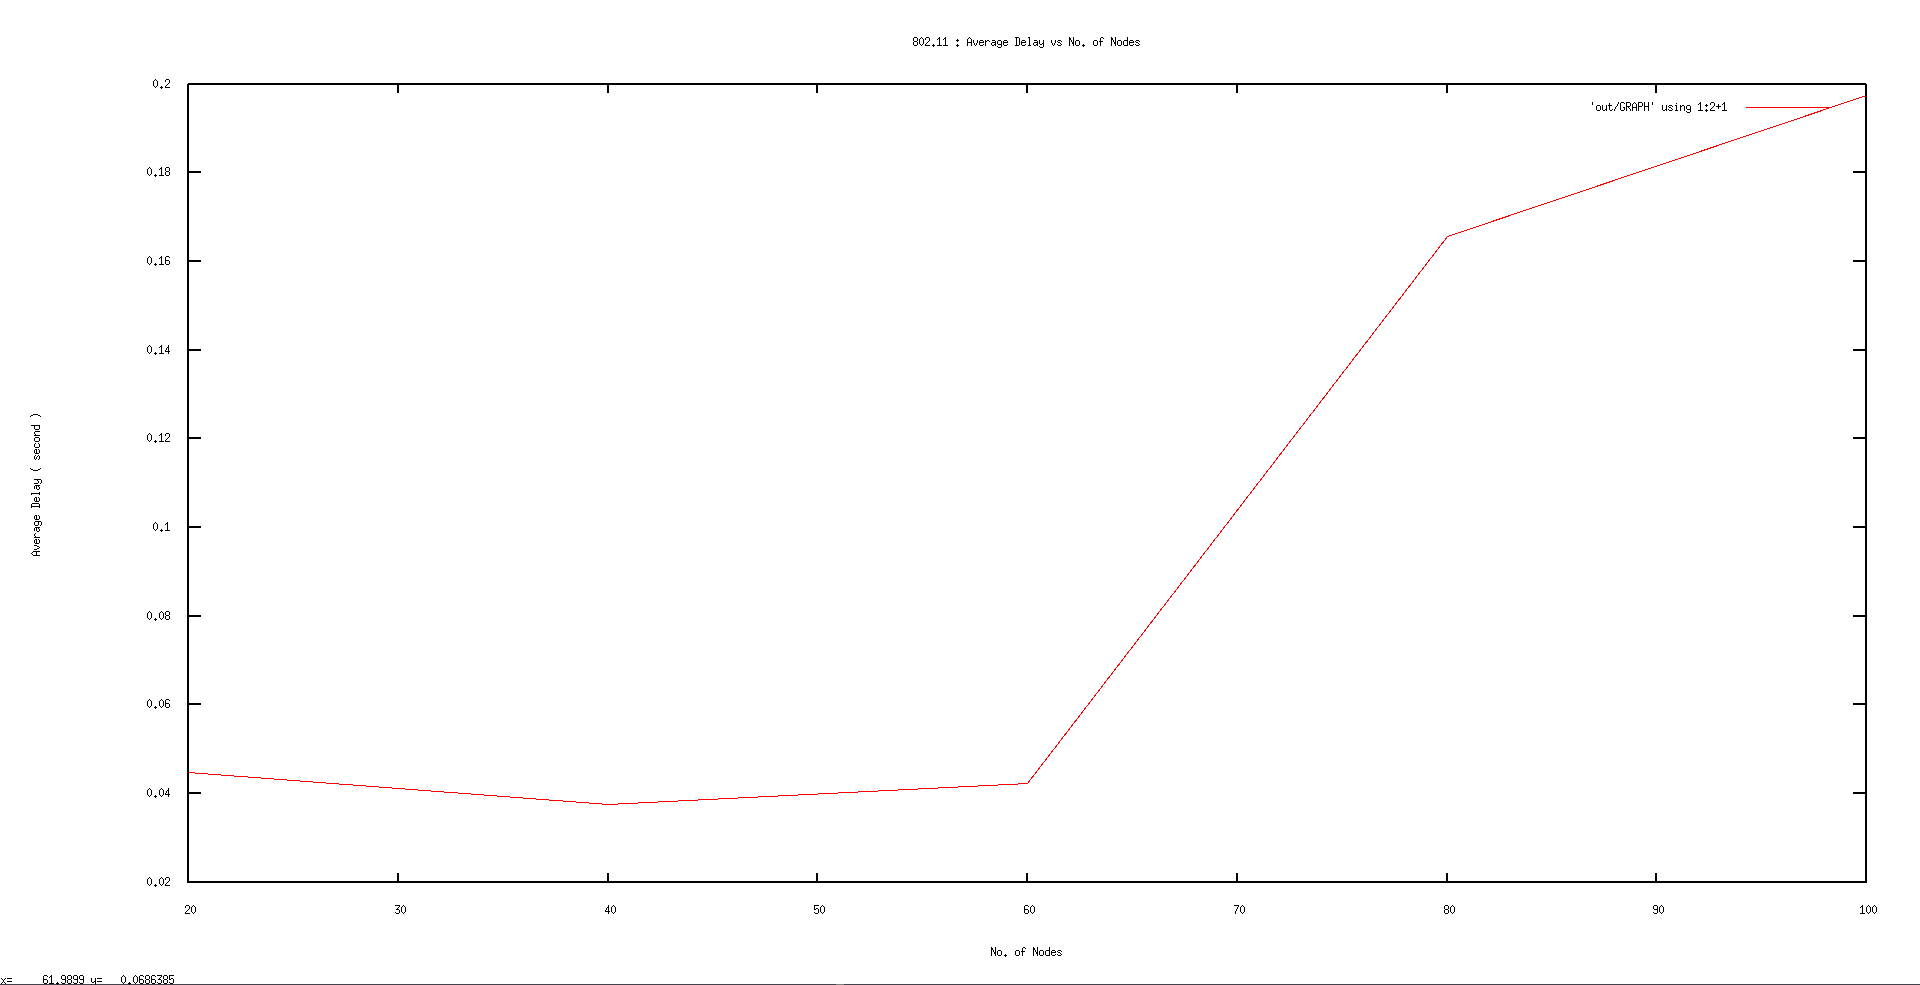
\includegraphics[scale=	0.26]{image/802.15.4/Averagedelay_vs_nodes.png}
\end{figure}

\begin{figure}[H]
	\centering
	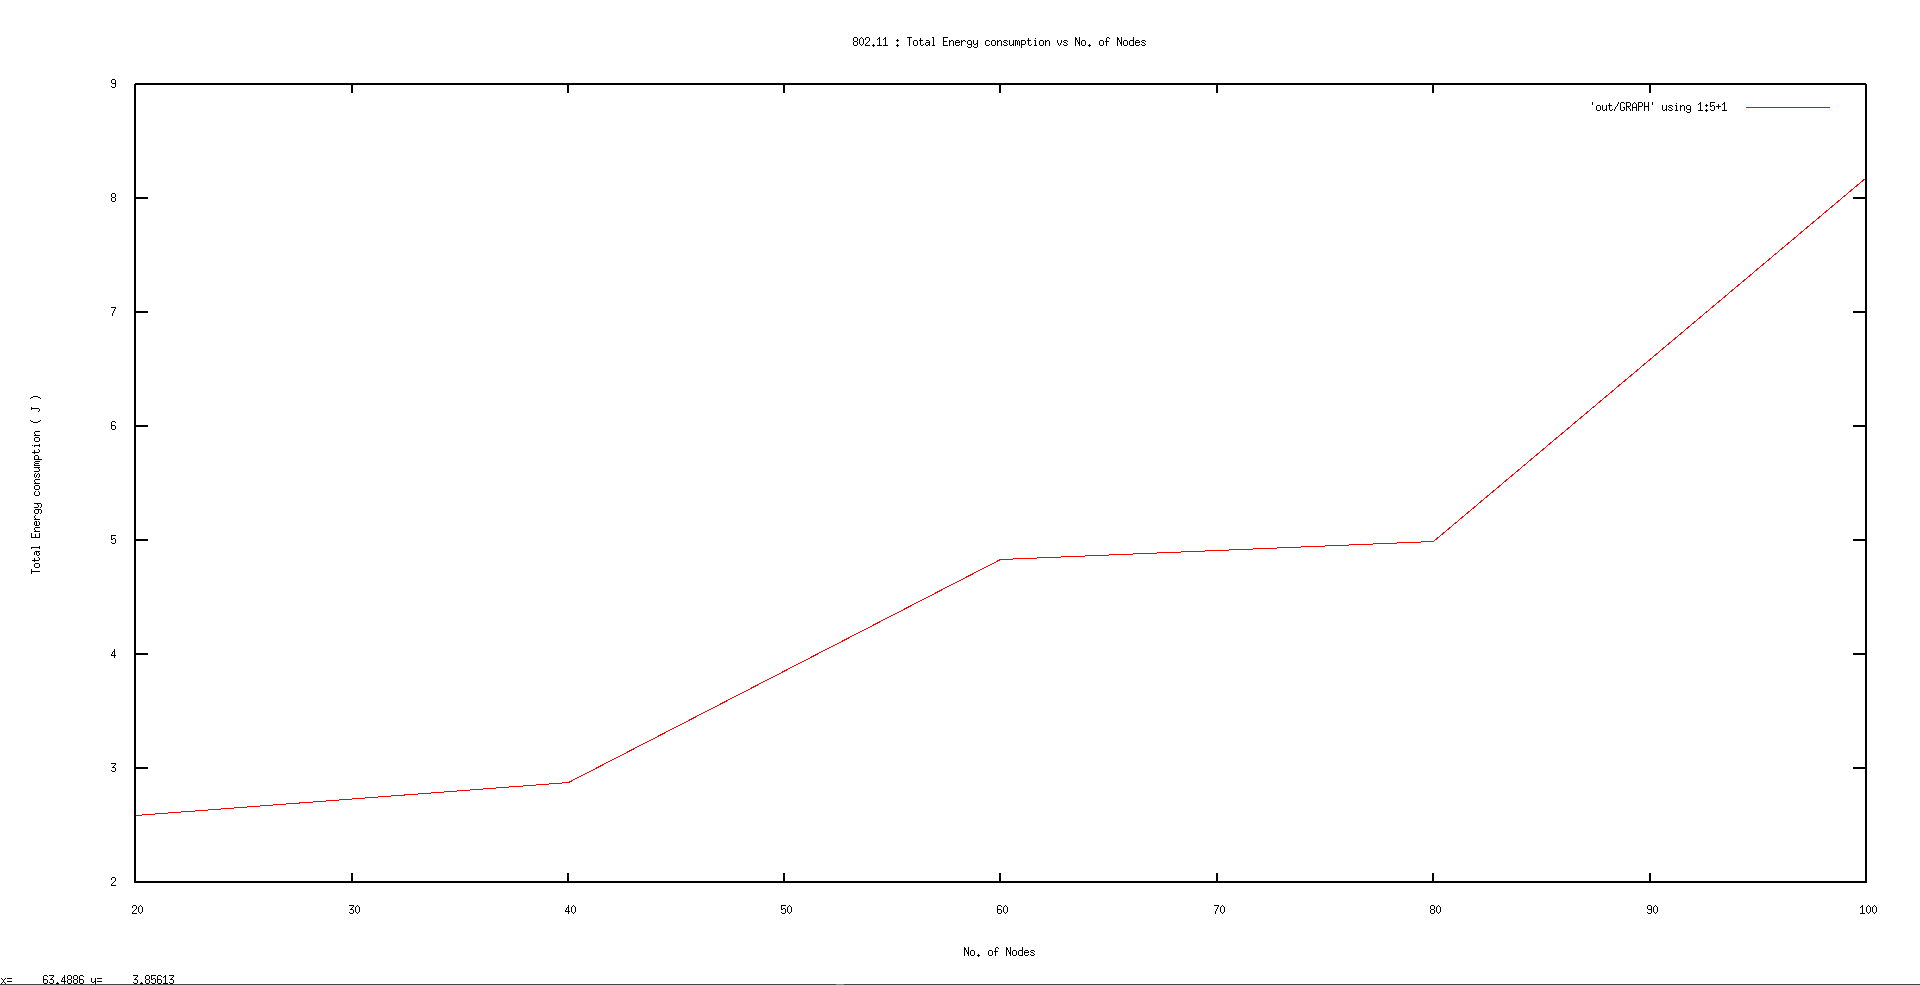
\includegraphics[scale=	0.26]{image/802.15.4/Energyconsumption_vs_nodes.png}
\end{figure}

\begin{figure}[H]
	\centering
	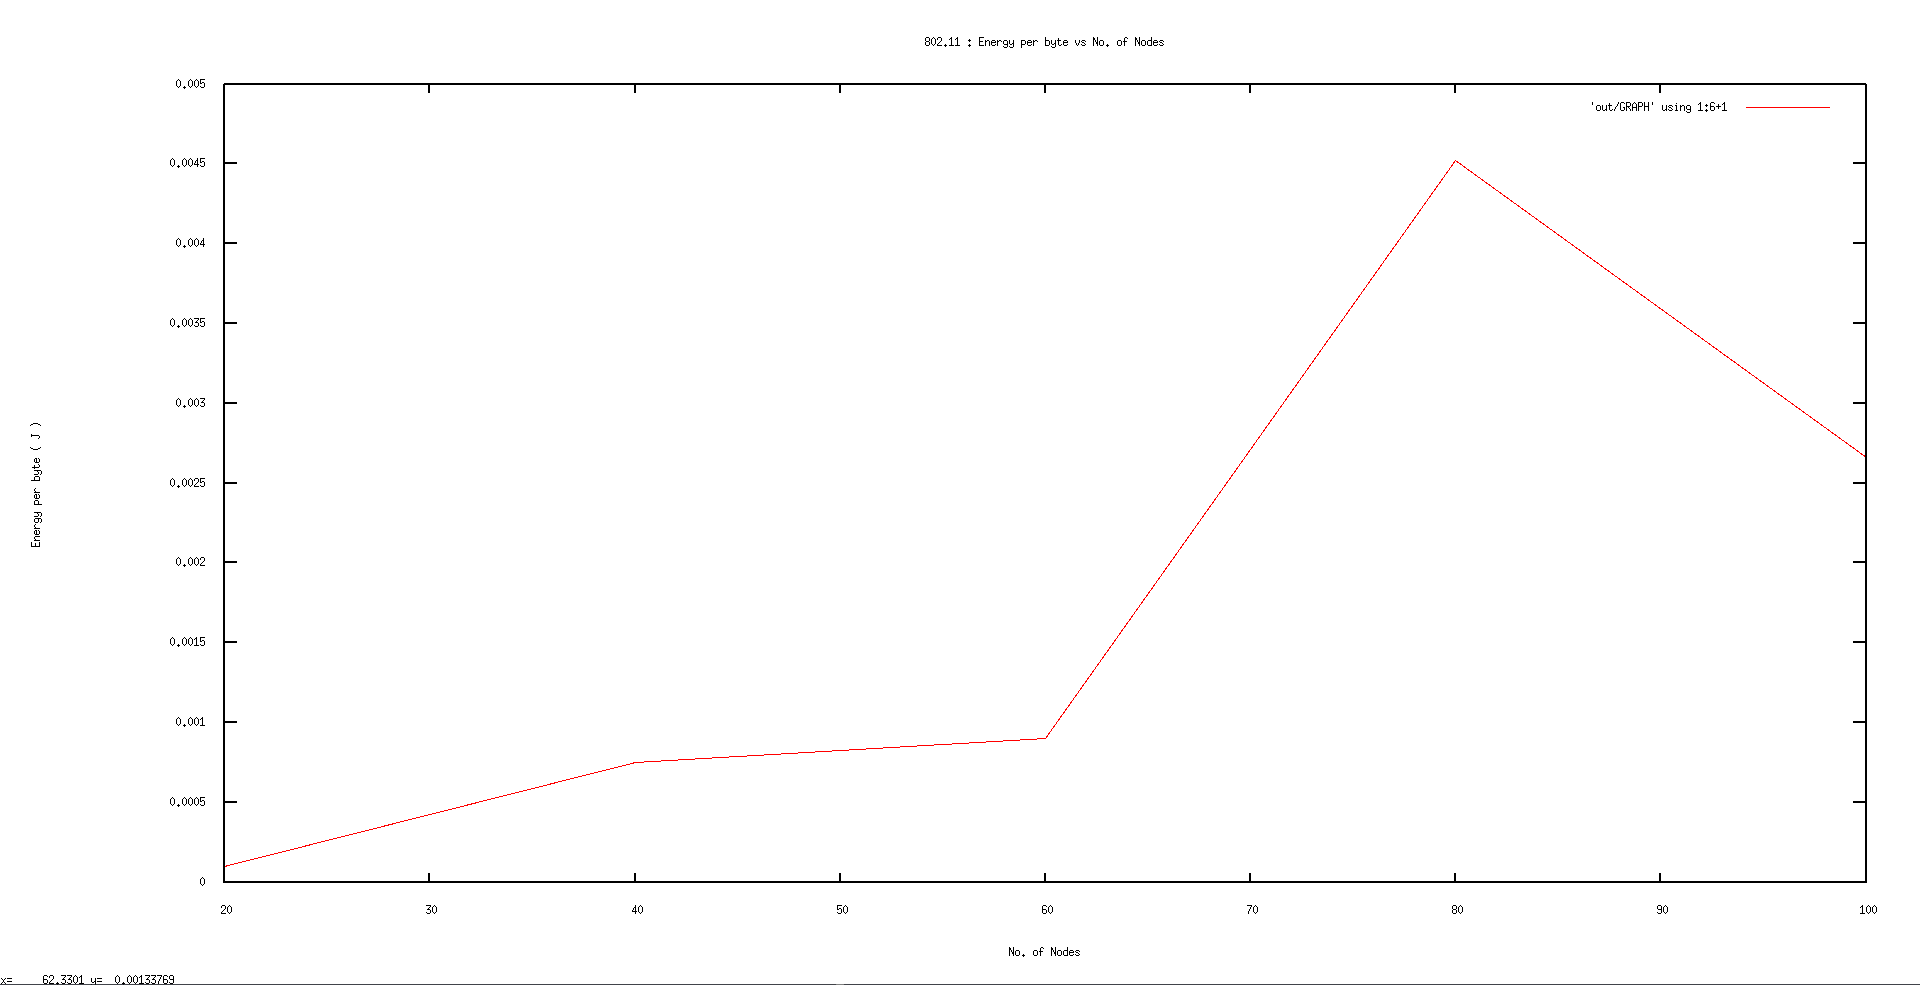
\includegraphics[scale=	0.26]{image/802.15.4/Energyperbytes_vs_nodes.png}
\end{figure}

\begin{figure}[H]
	\centering
	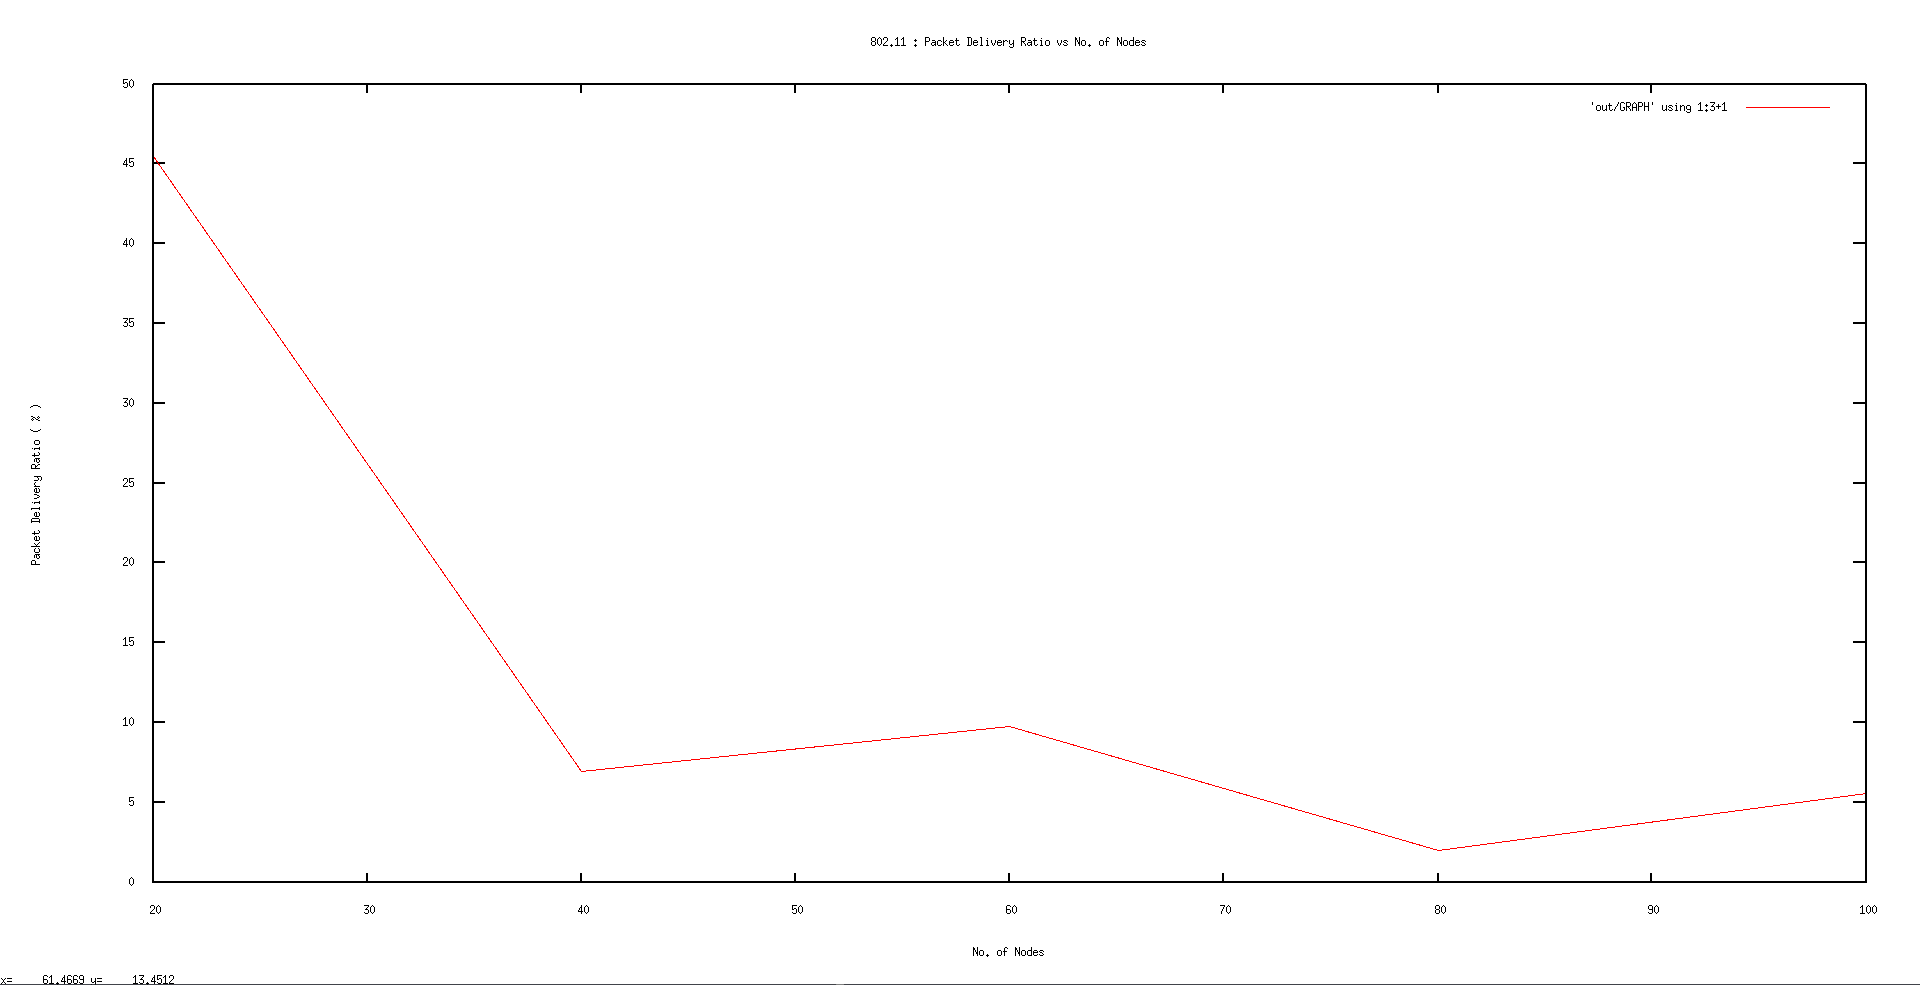
\includegraphics[scale=	0.26]{image/802.15.4/Packetdeliveryratio_vs_nodes.png}
\end{figure}

\begin{figure}[H]
	\centering
	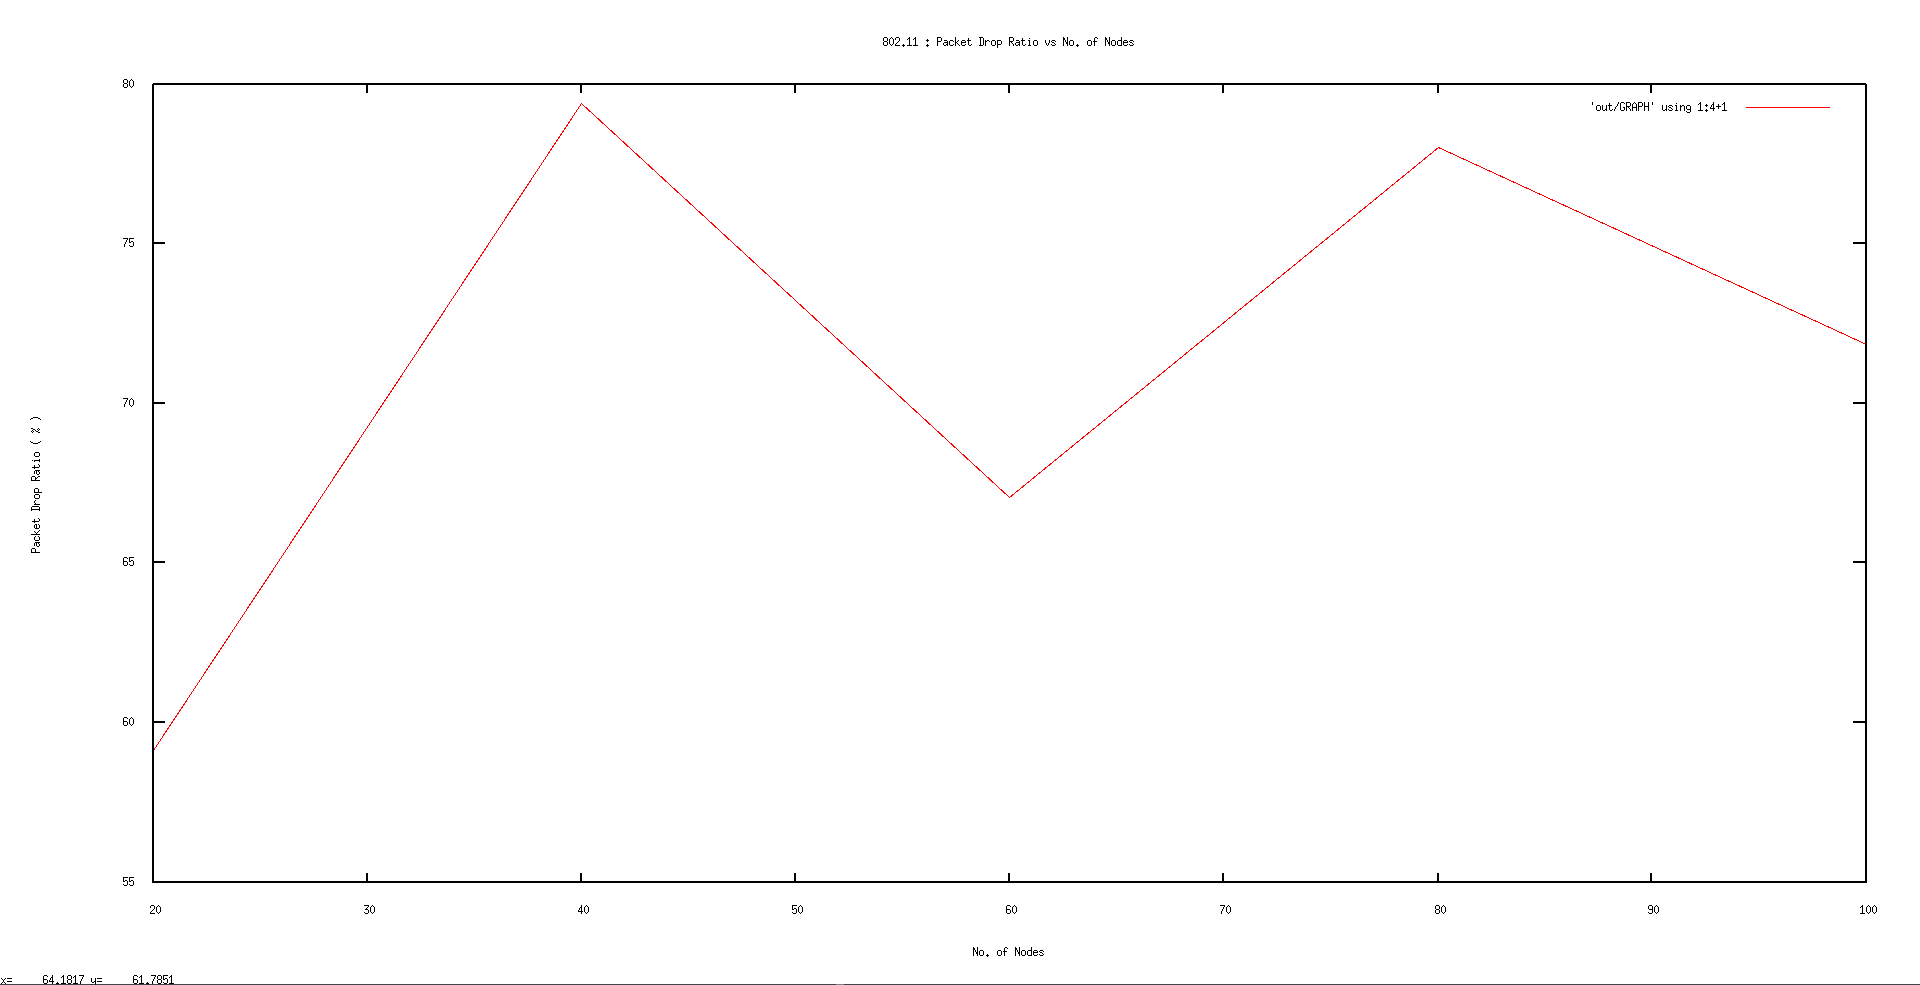
\includegraphics[scale=	0.26]{image/802.15.4/Packetdropratio_vs_nodes.png}
\end{figure}


\newpage
\title{Variation in Number of Flow}
\begin{figure}[H]
	\centering
	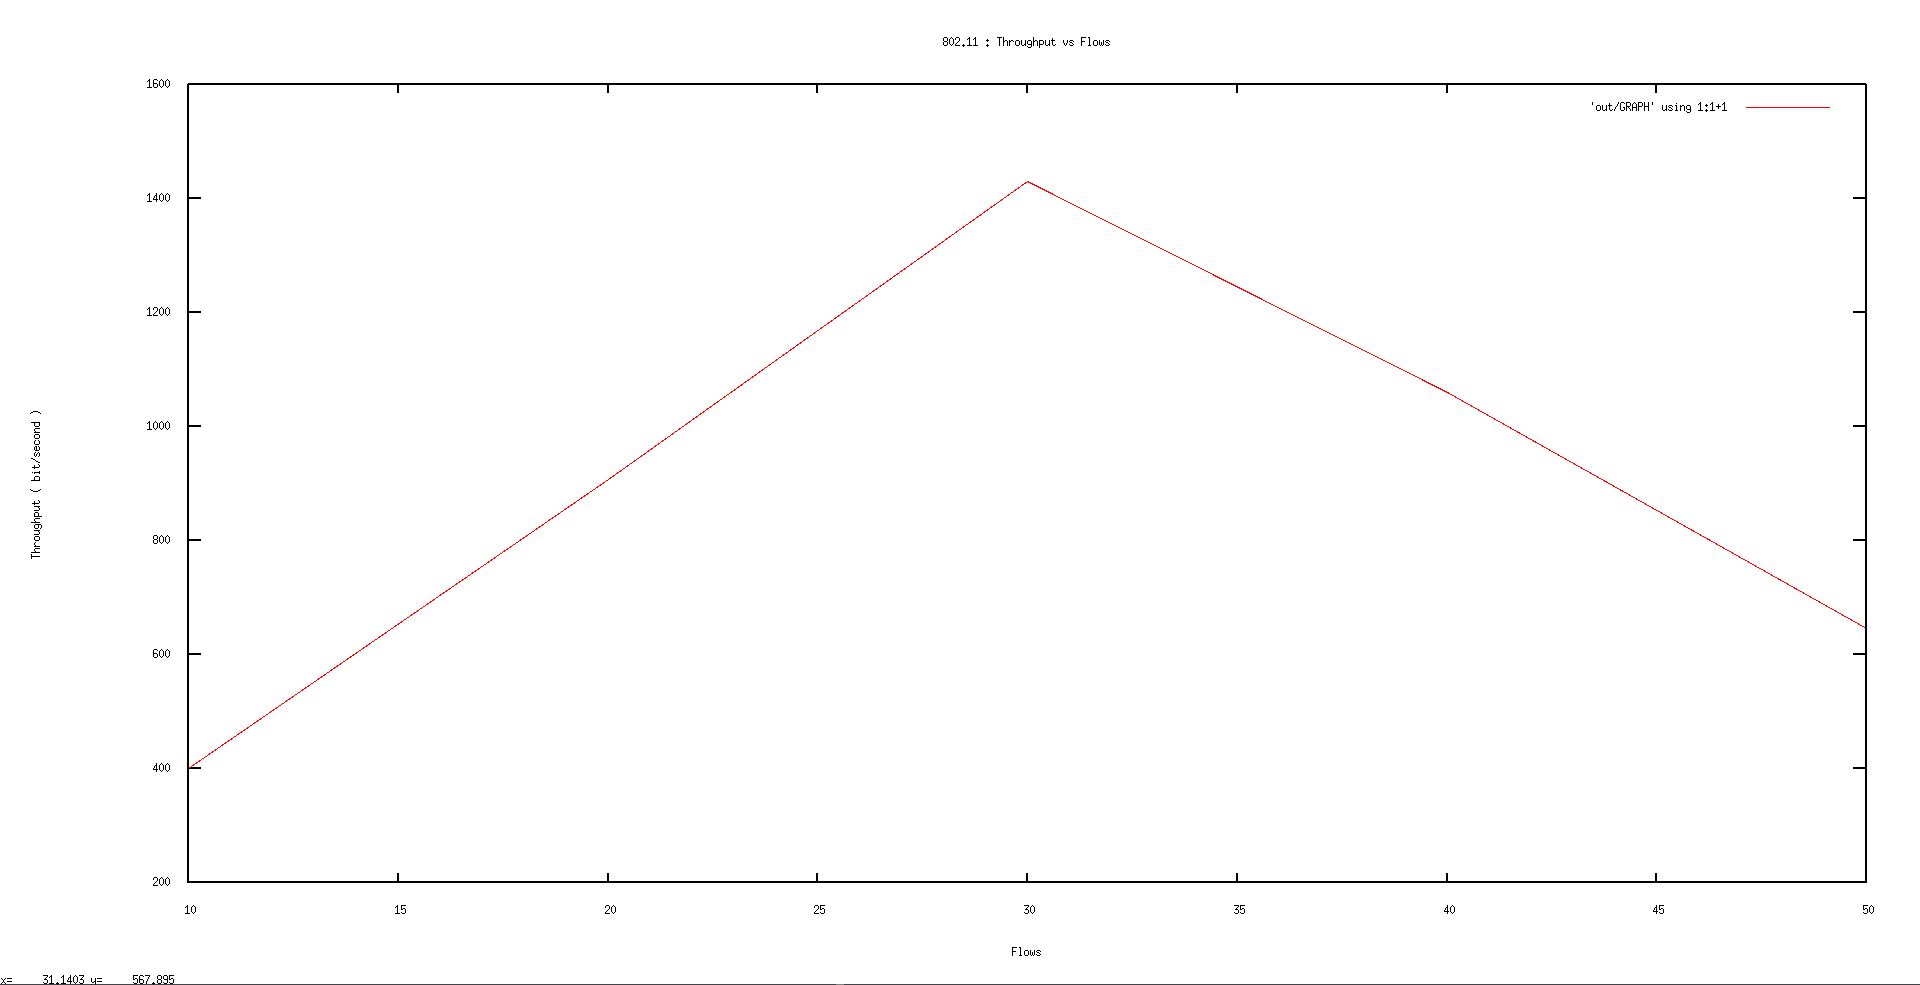
\includegraphics[scale=	0.26]{image/802.15.4/Throughput_vs_flows.png}
\end{figure}

\begin{figure}[H]
	\centering
	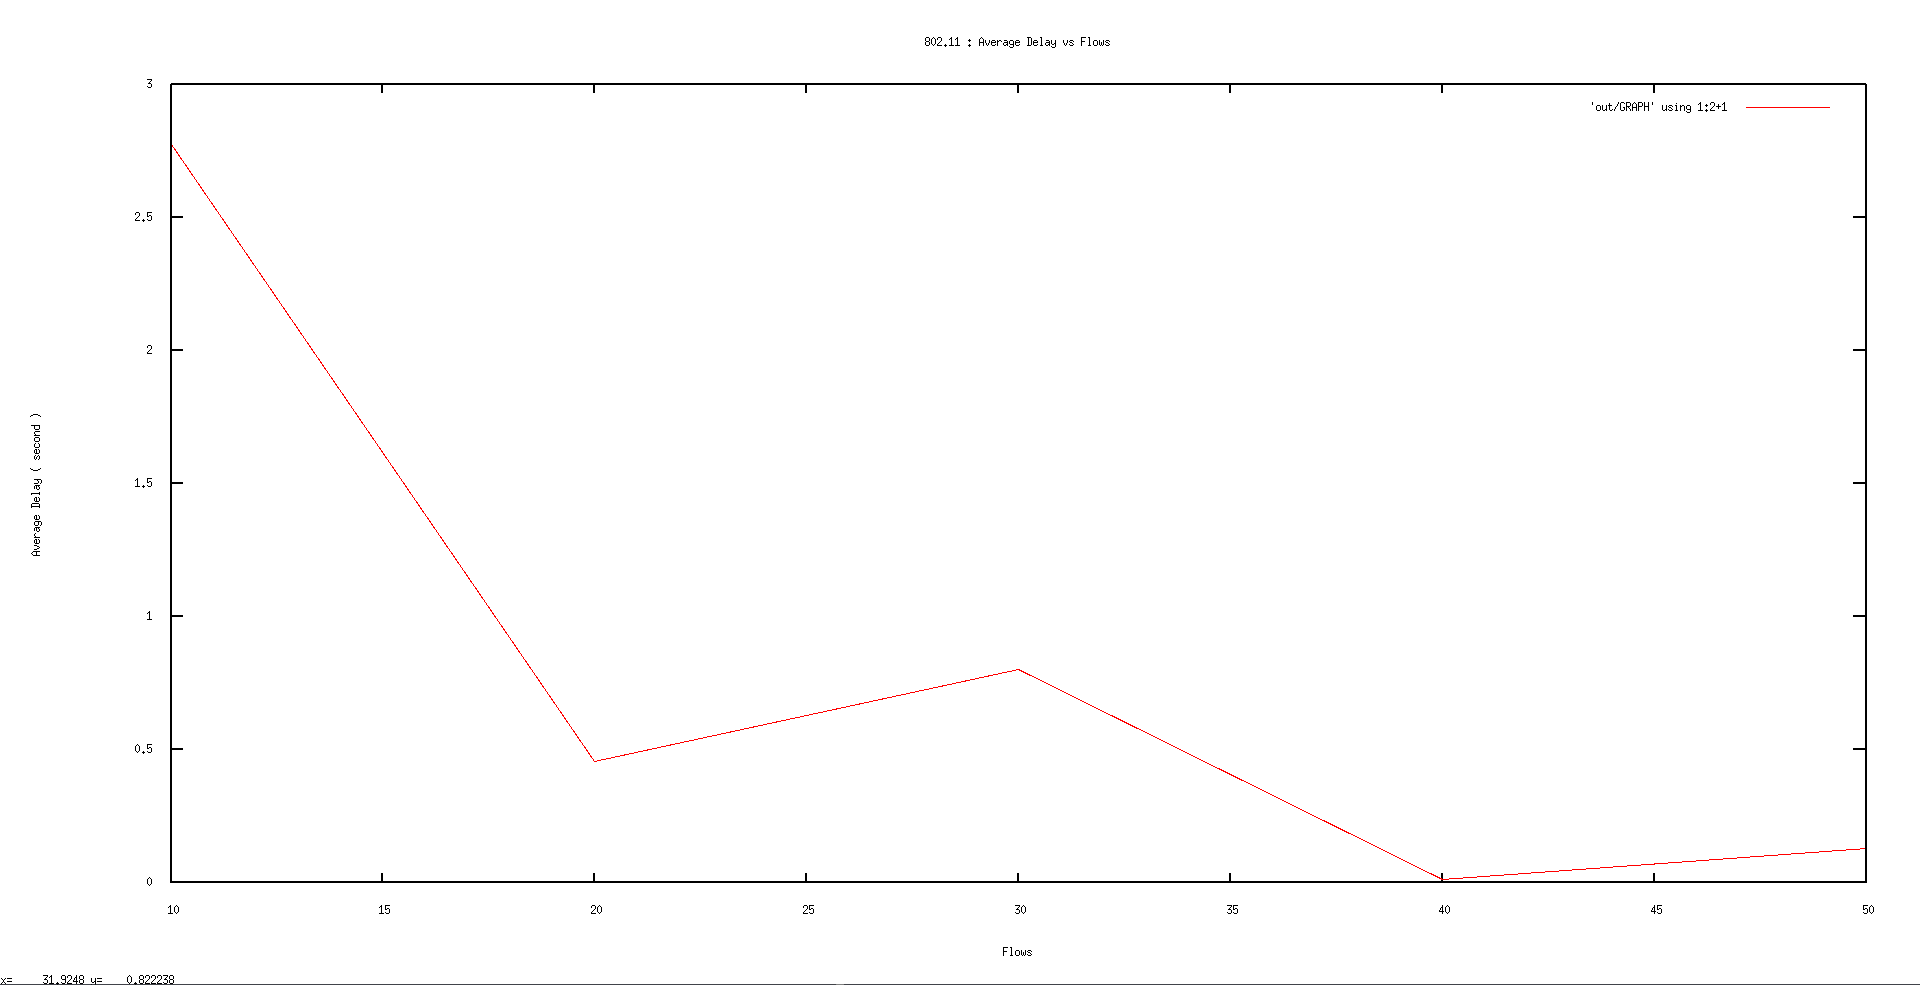
\includegraphics[scale=	0.26]{image/802.15.4/Averagedelay_vs_flows.png}
\end{figure}

\begin{figure}[H]
	\centering
	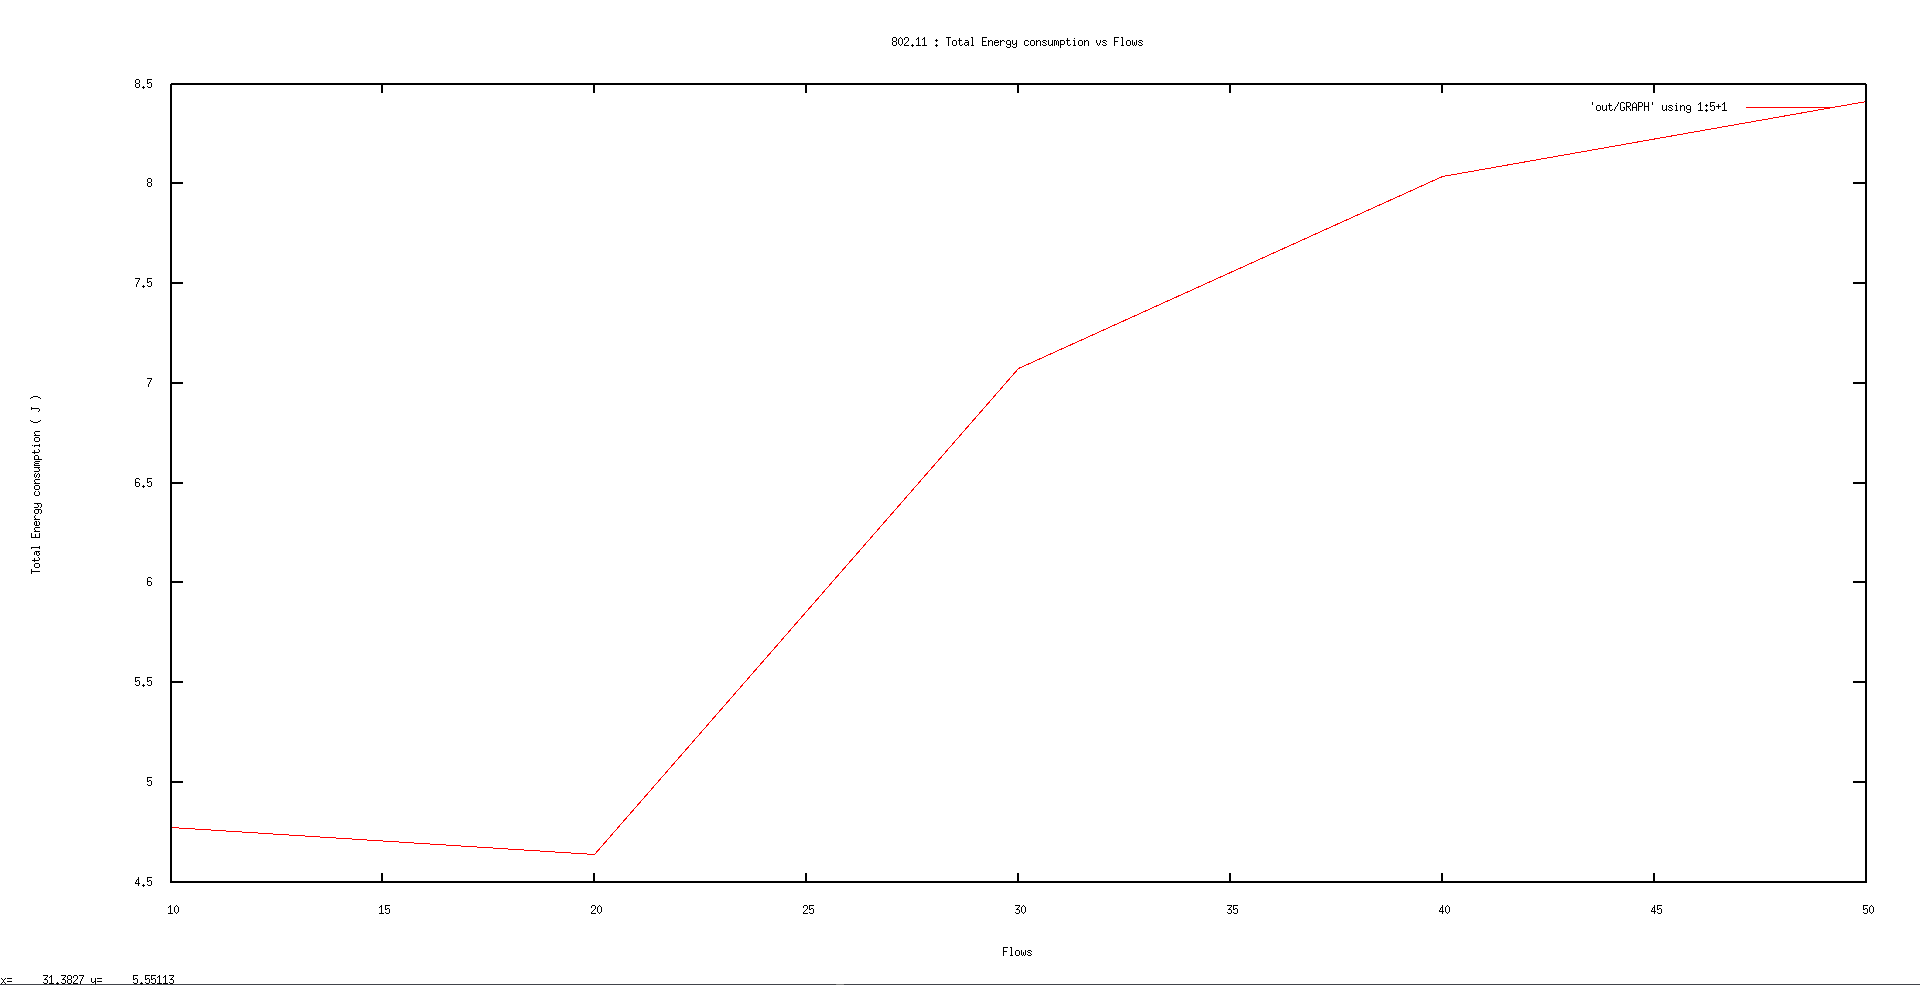
\includegraphics[scale=	0.26]{image/802.15.4/Energyconsumption_vs_flows.png}
\end{figure}

\begin{figure}[H]
	\centering
	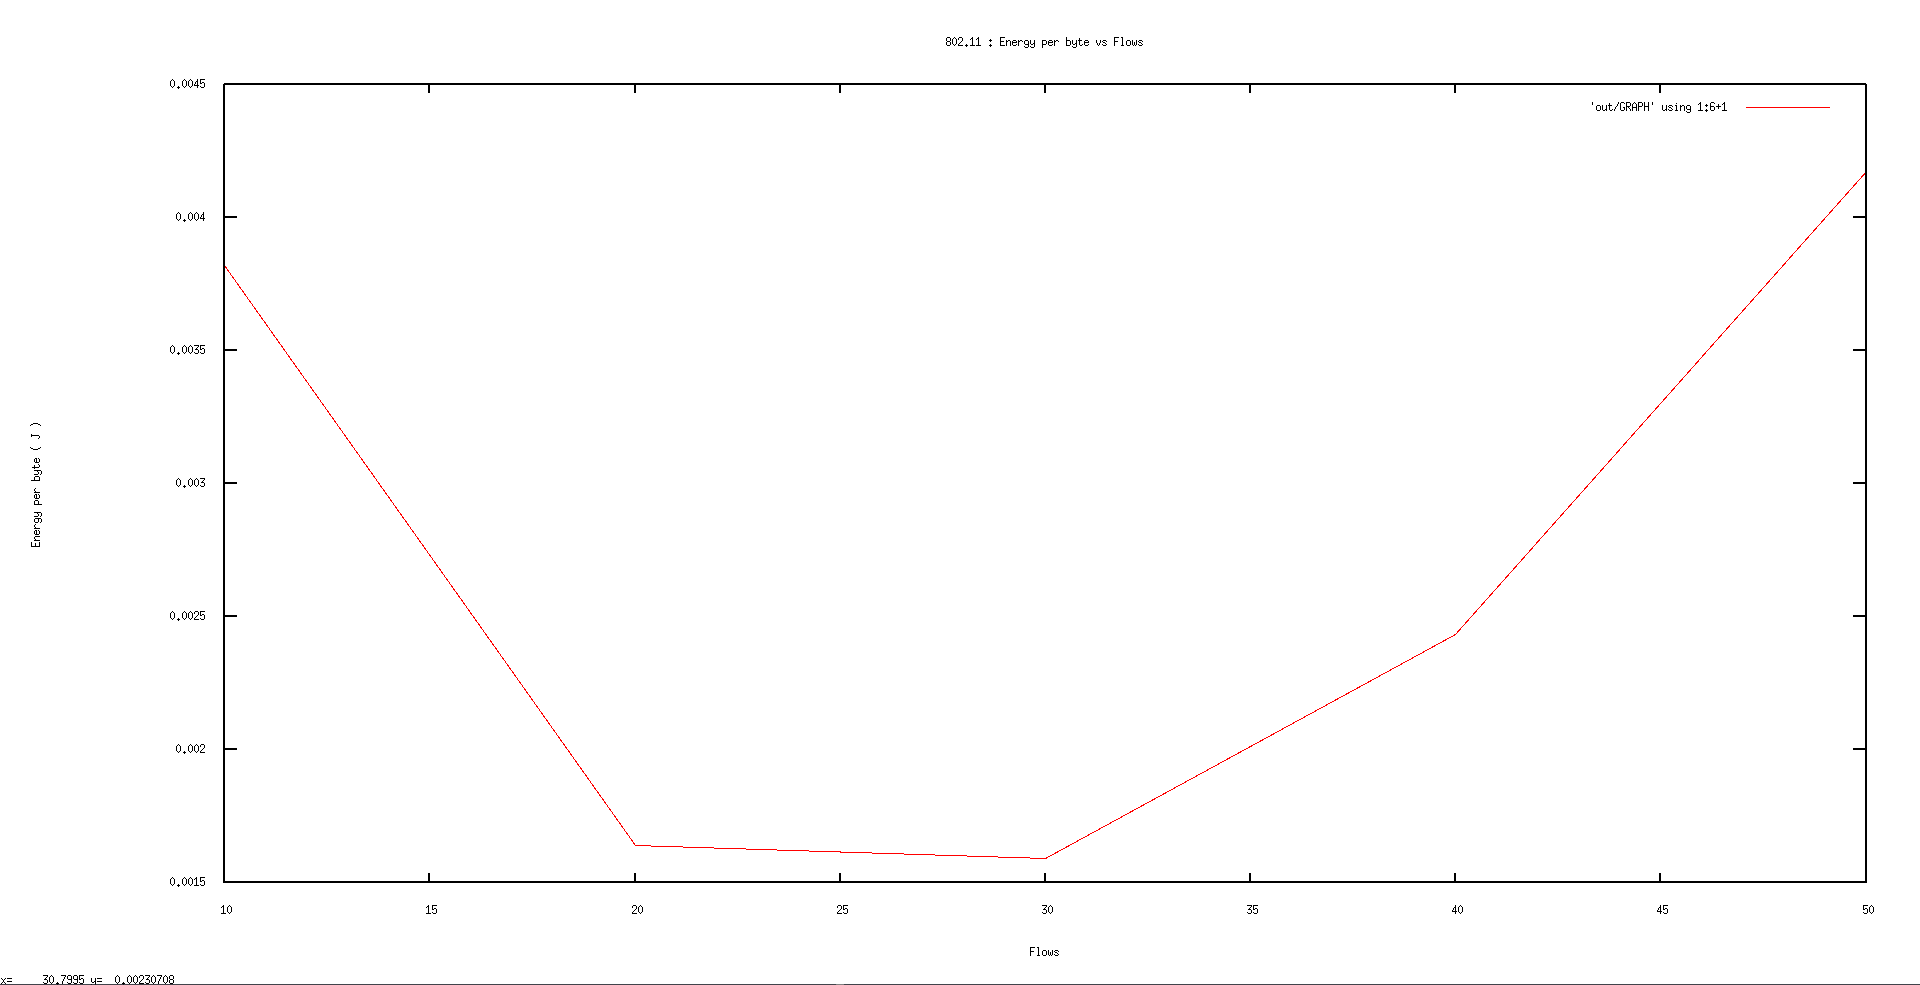
\includegraphics[scale=	0.26]{image/802.15.4/Energyperbytes_vs_flows.png}
\end{figure}

\begin{figure}[H]
	\centering
	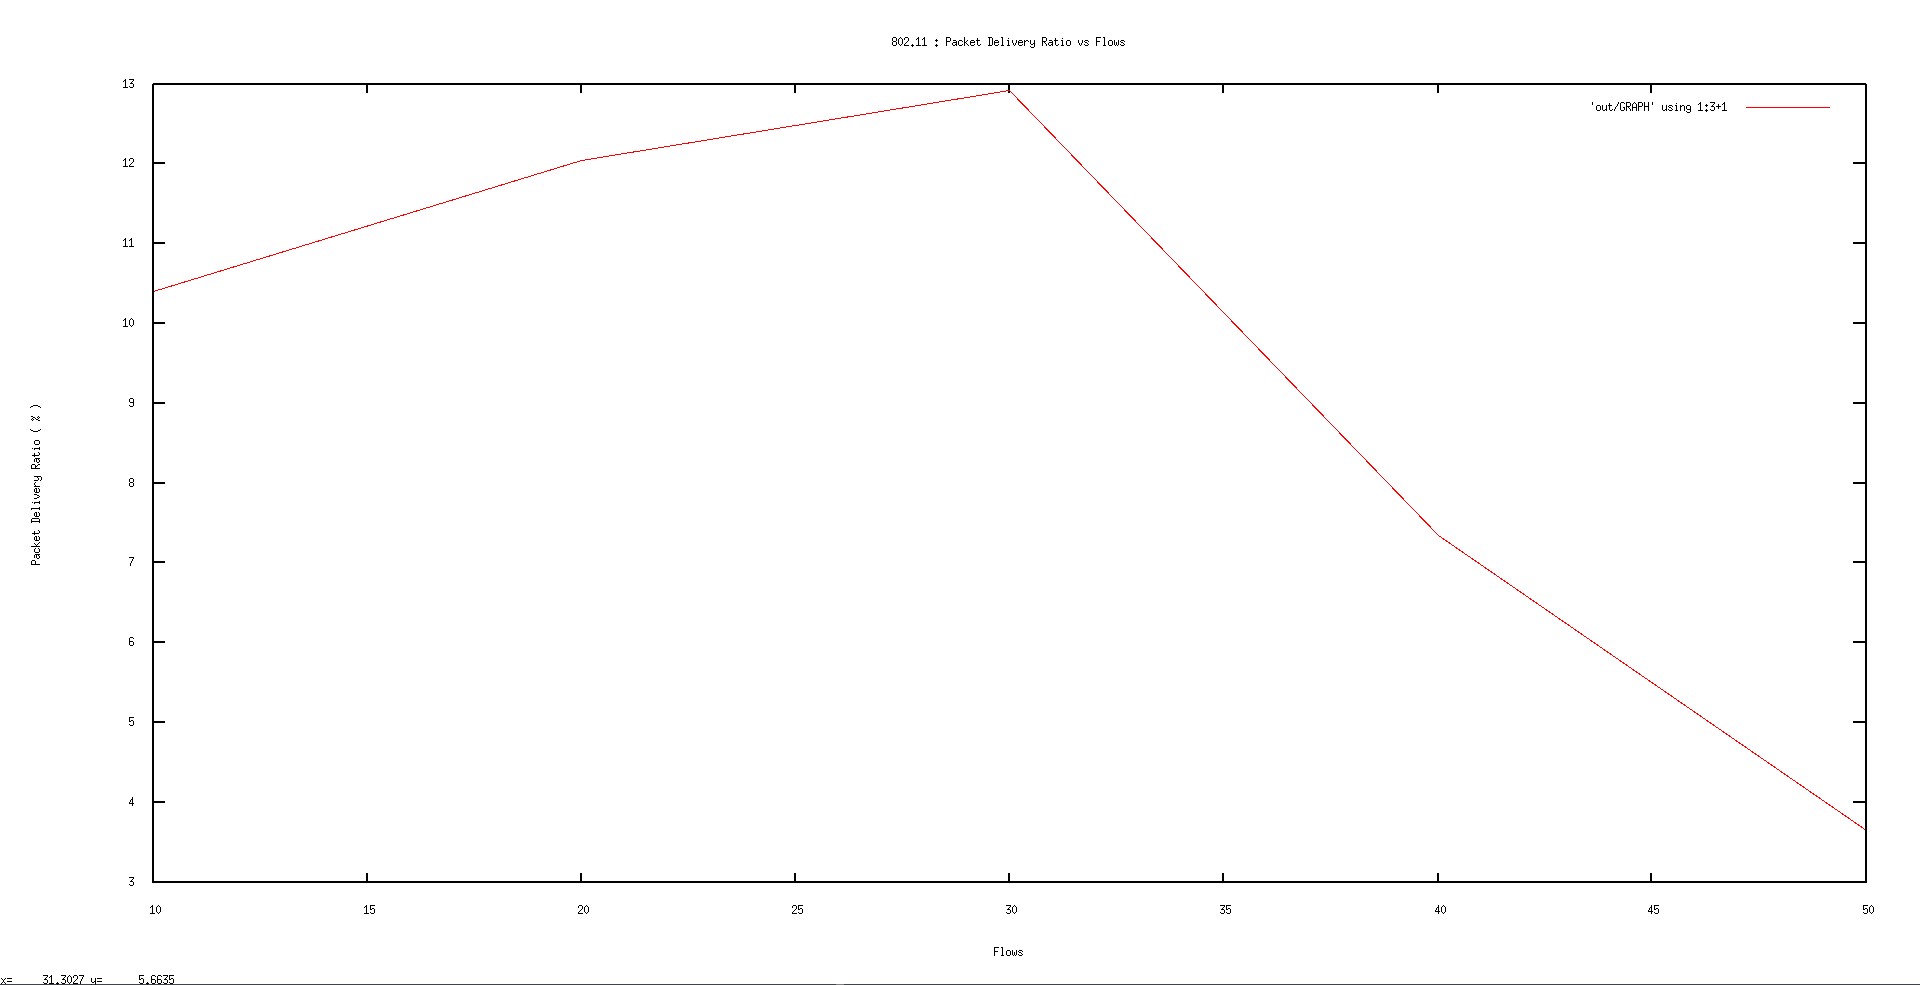
\includegraphics[scale=	0.26]{image/802.15.4/Packetdeliveryratio_vs_flows.png}
\end{figure}

\begin{figure}[H]
	\centering
	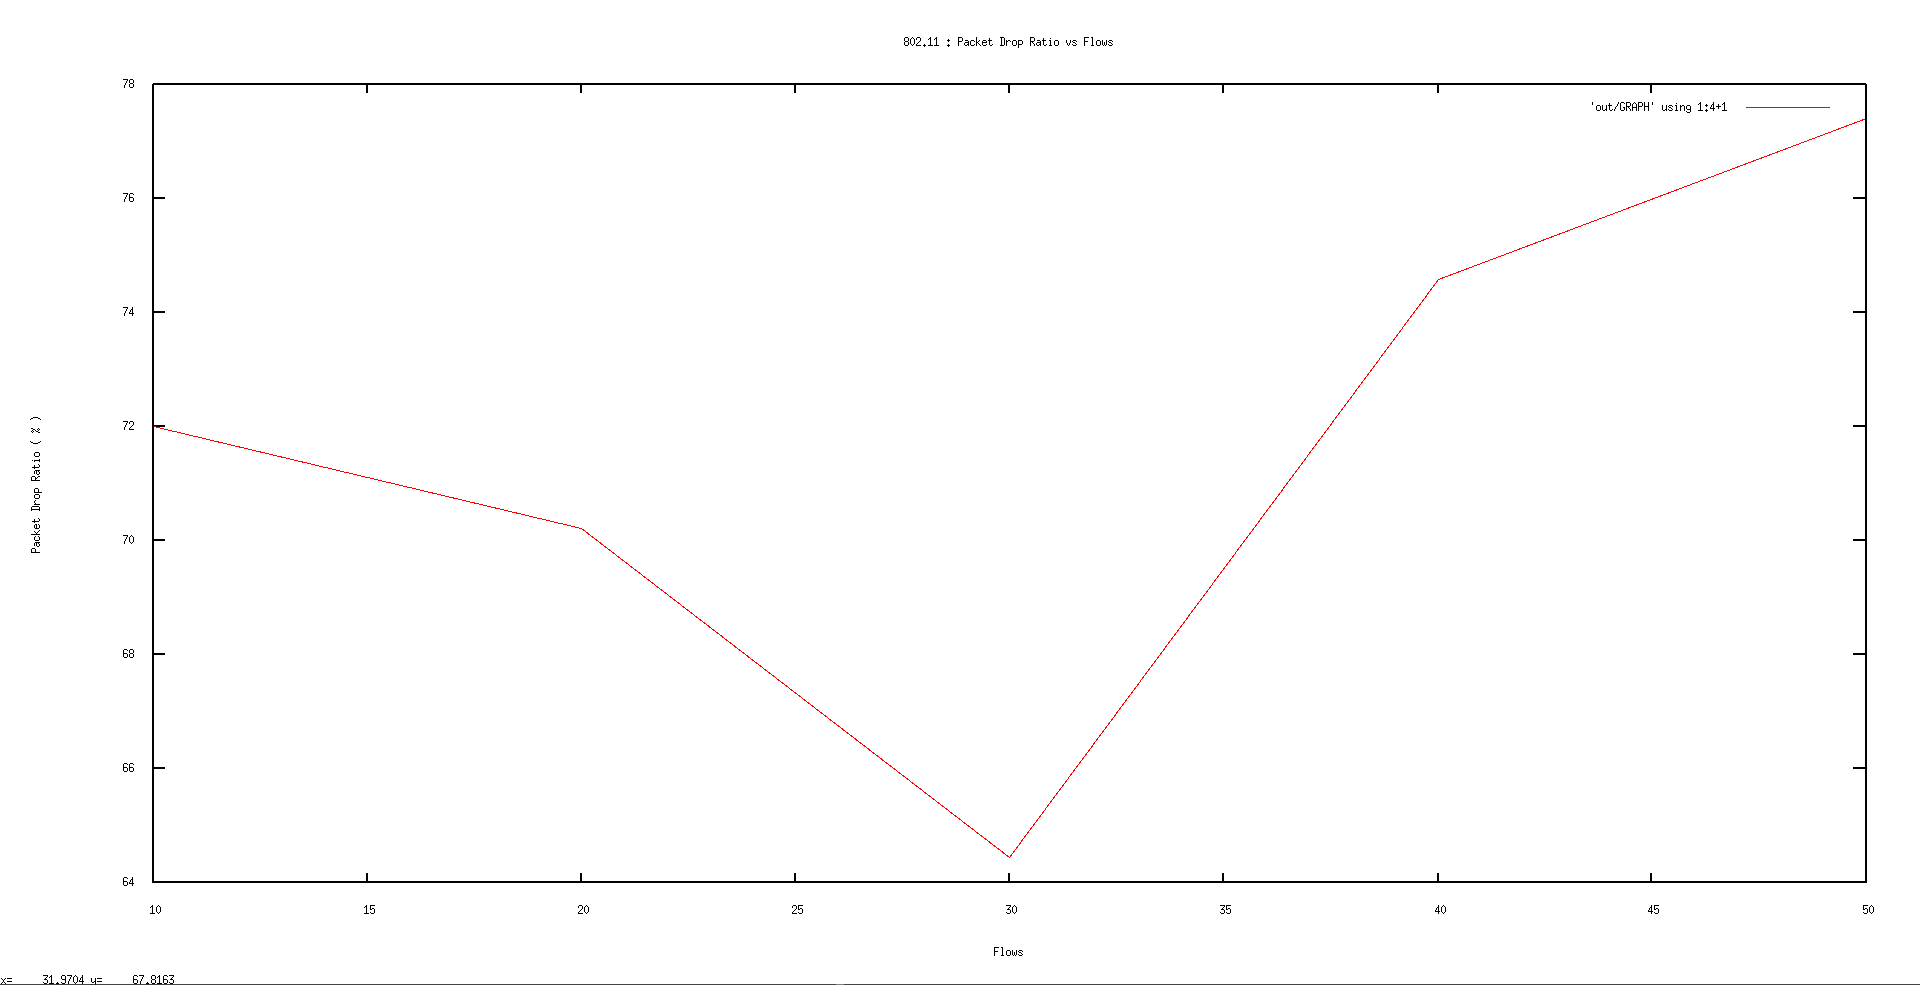
\includegraphics[scale=	0.26]{image/802.15.4/Packetdropratio_vs_flows.png}
\end{figure}


\newpage
\title{Variation in Packets Sent per Second}
\begin{figure}[H]
	\centering
	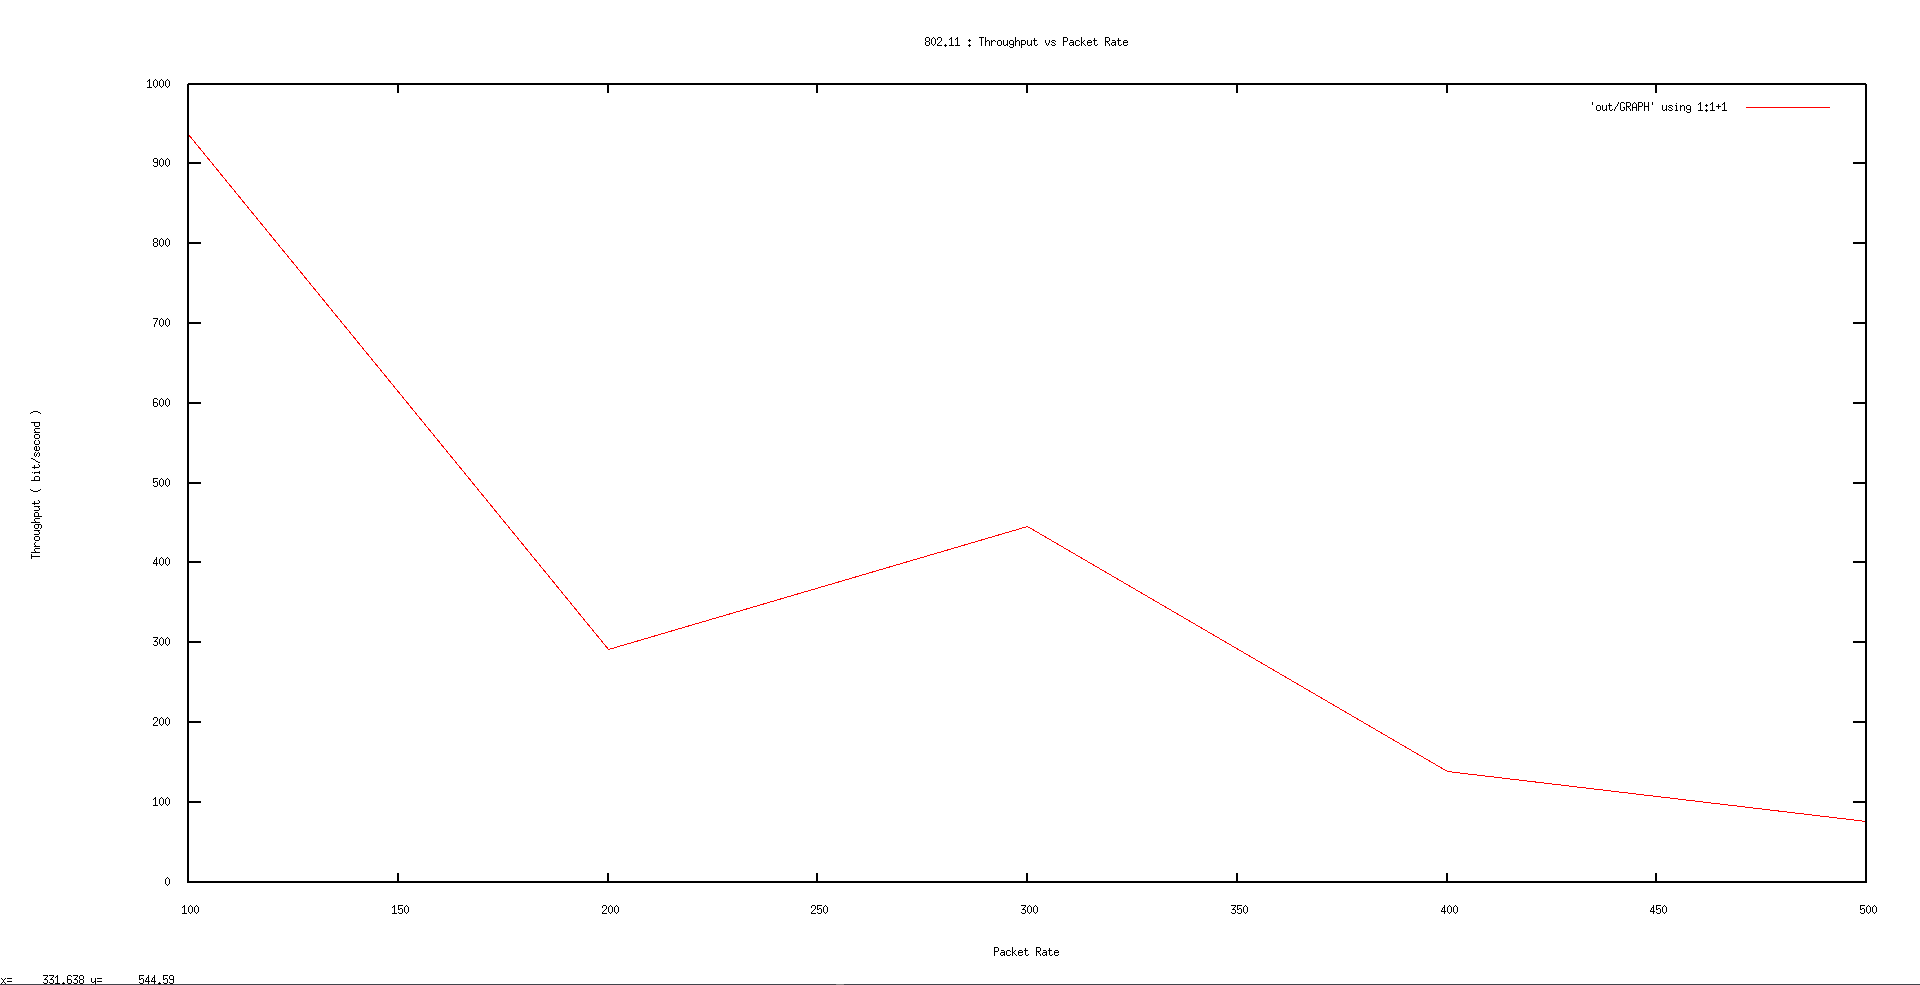
\includegraphics[scale=	0.26]{image/802.15.4/Throughput_vs_packetRates.png}
\end{figure}

\begin{figure}[H]
	\centering
	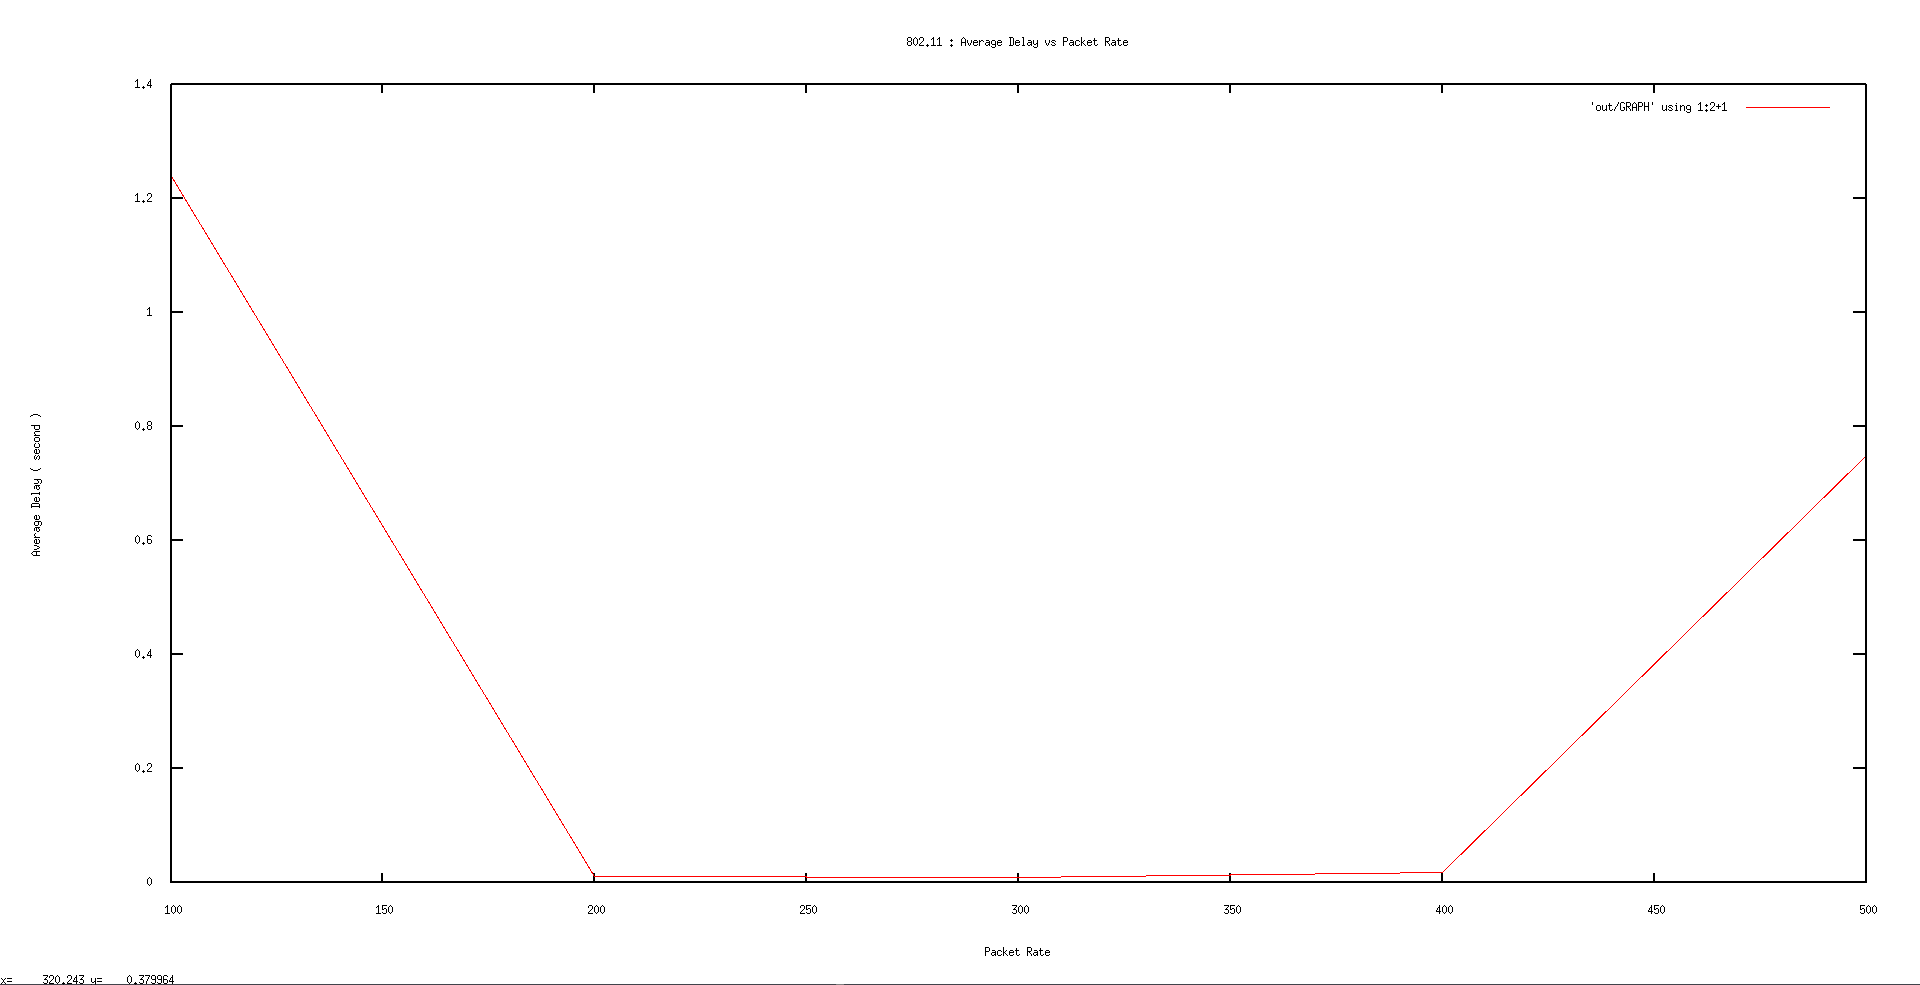
\includegraphics[scale=	0.26]{image/802.15.4/Averagedelay_vs_packetRates.png}
\end{figure}

\begin{figure}[H]
	\centering
	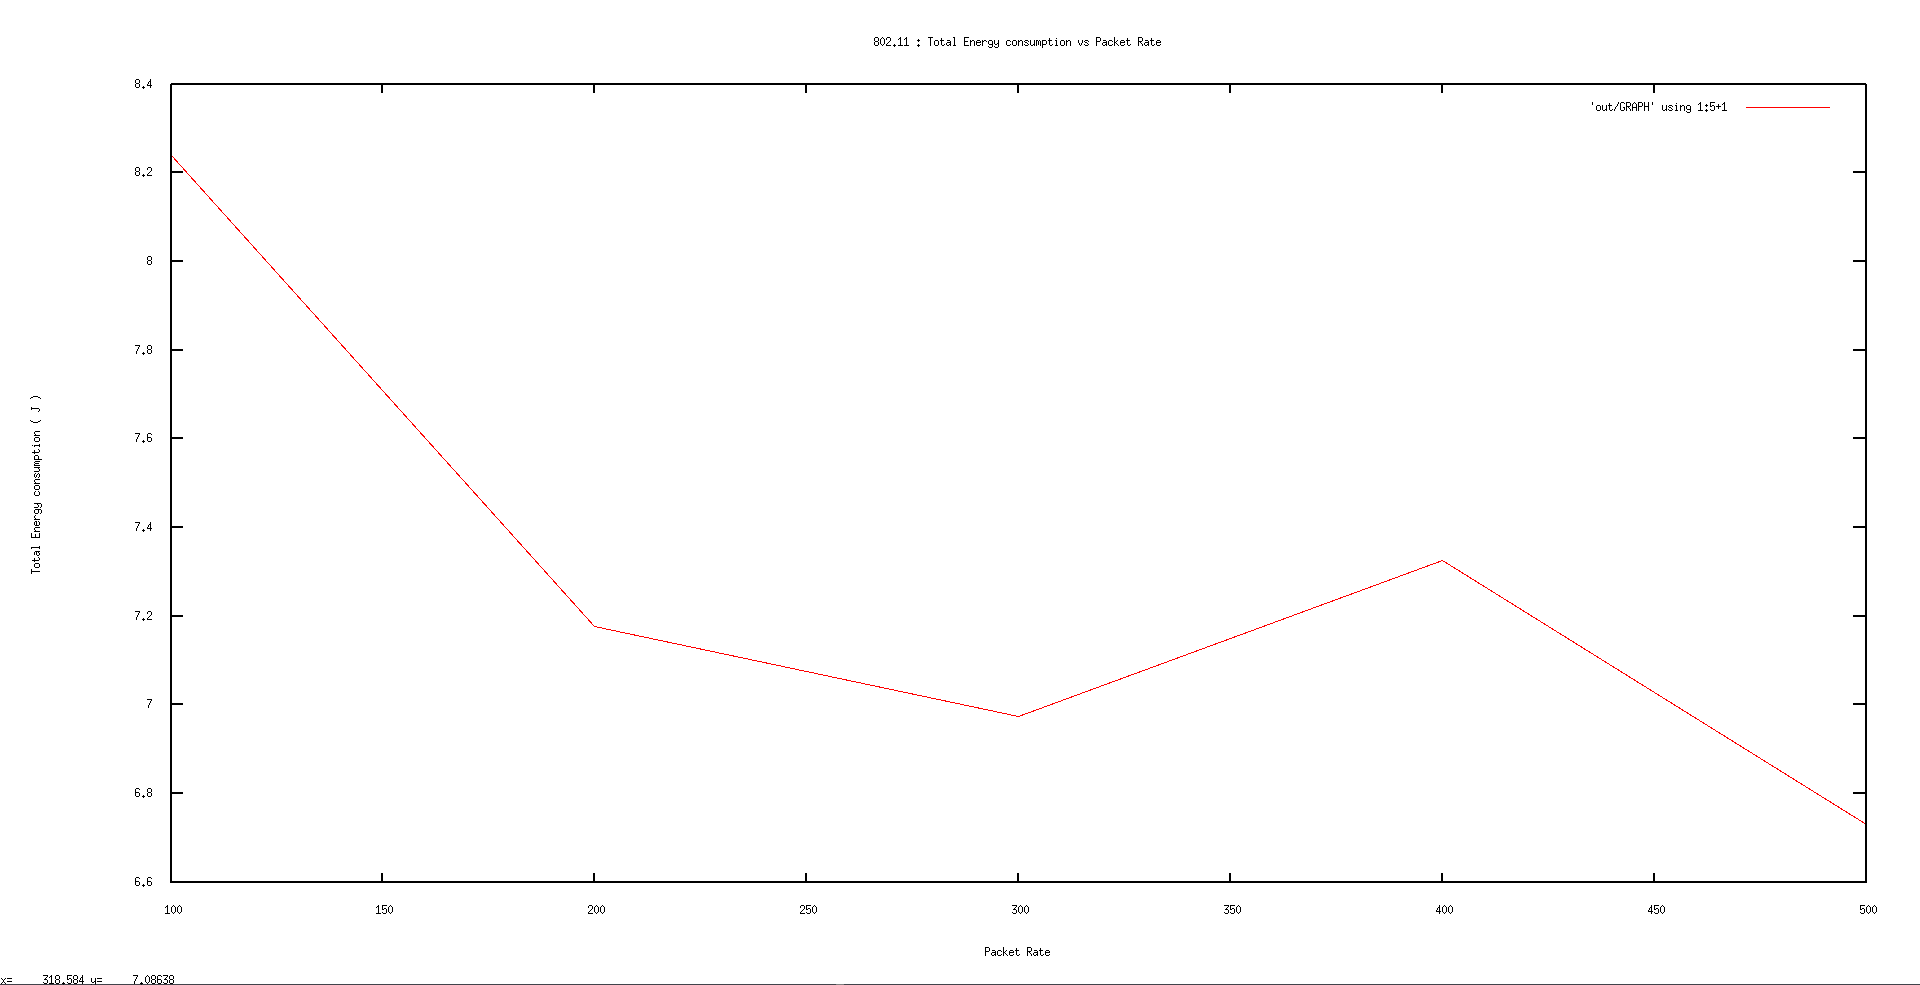
\includegraphics[scale=	0.26]{image/802.15.4/Energyconsumption_vs_packetRates.png}
\end{figure}

\begin{figure}[H]
	\centering
	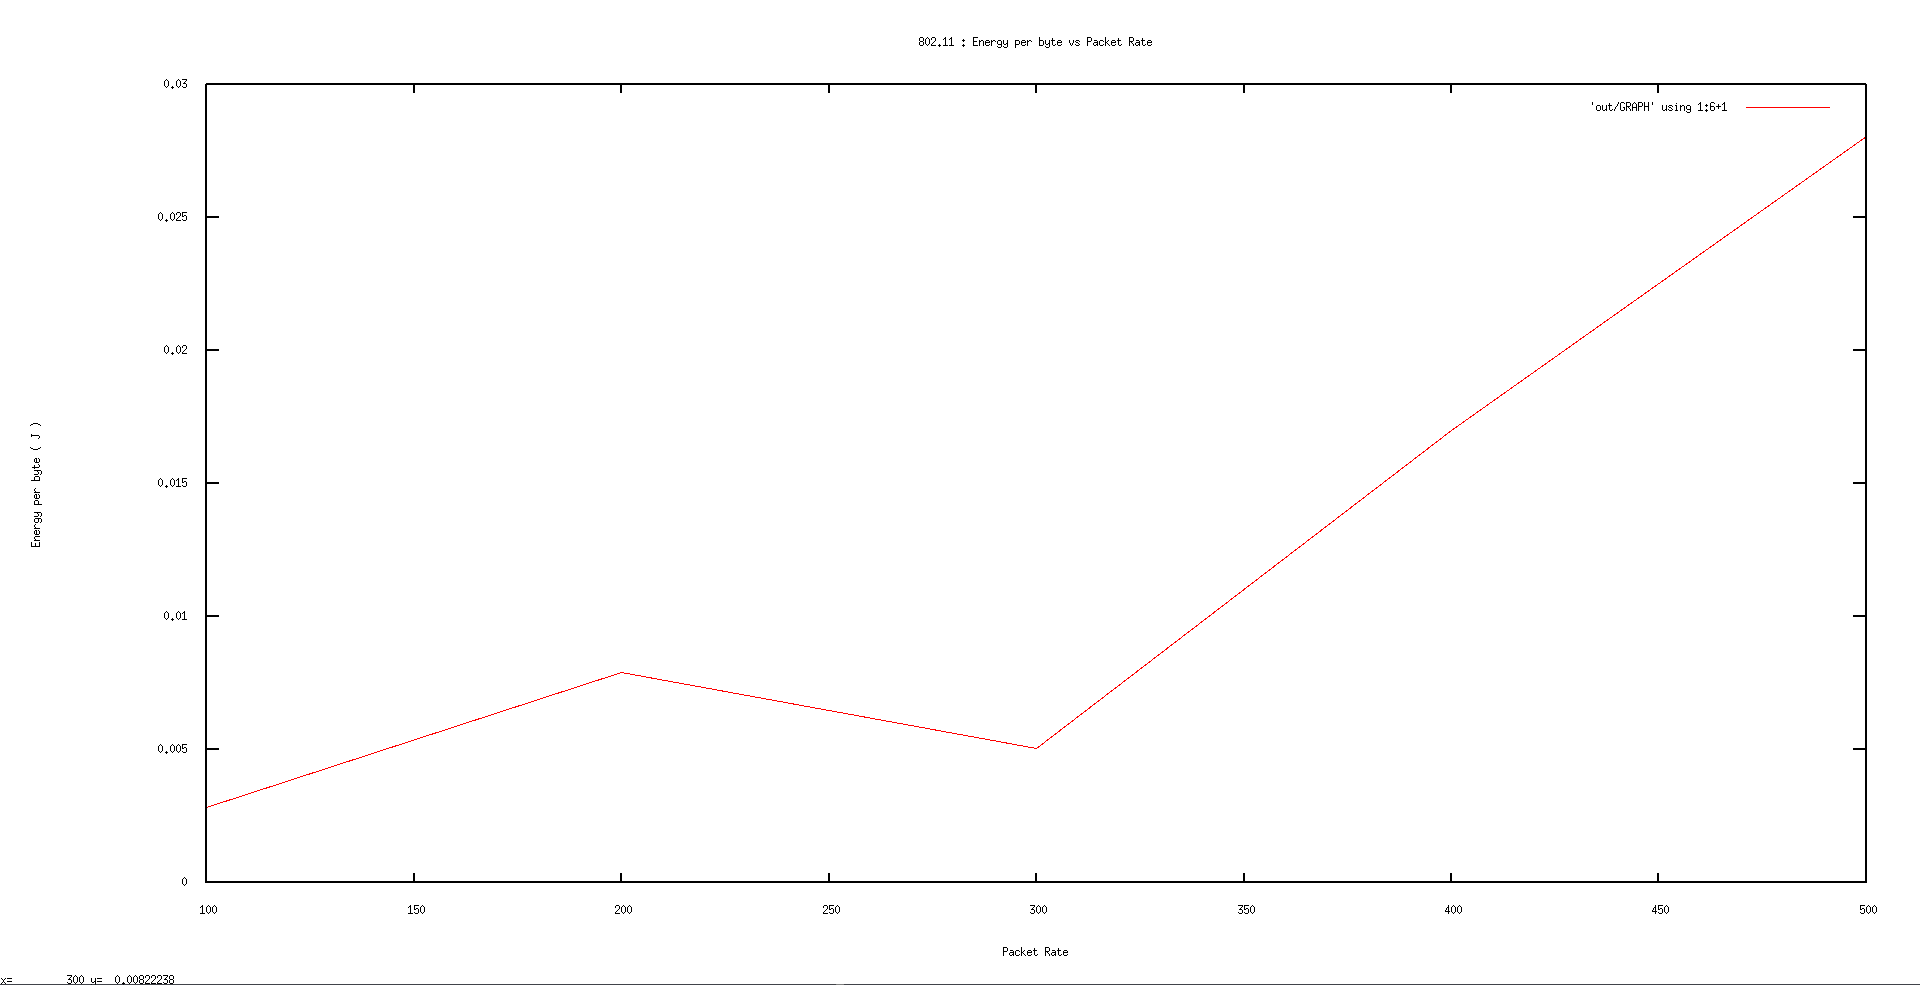
\includegraphics[scale=	0.26]{image/802.15.4/Energyperbytes_vs_packetRates.png}
\end{figure}

\begin{figure}[H]
	\centering
	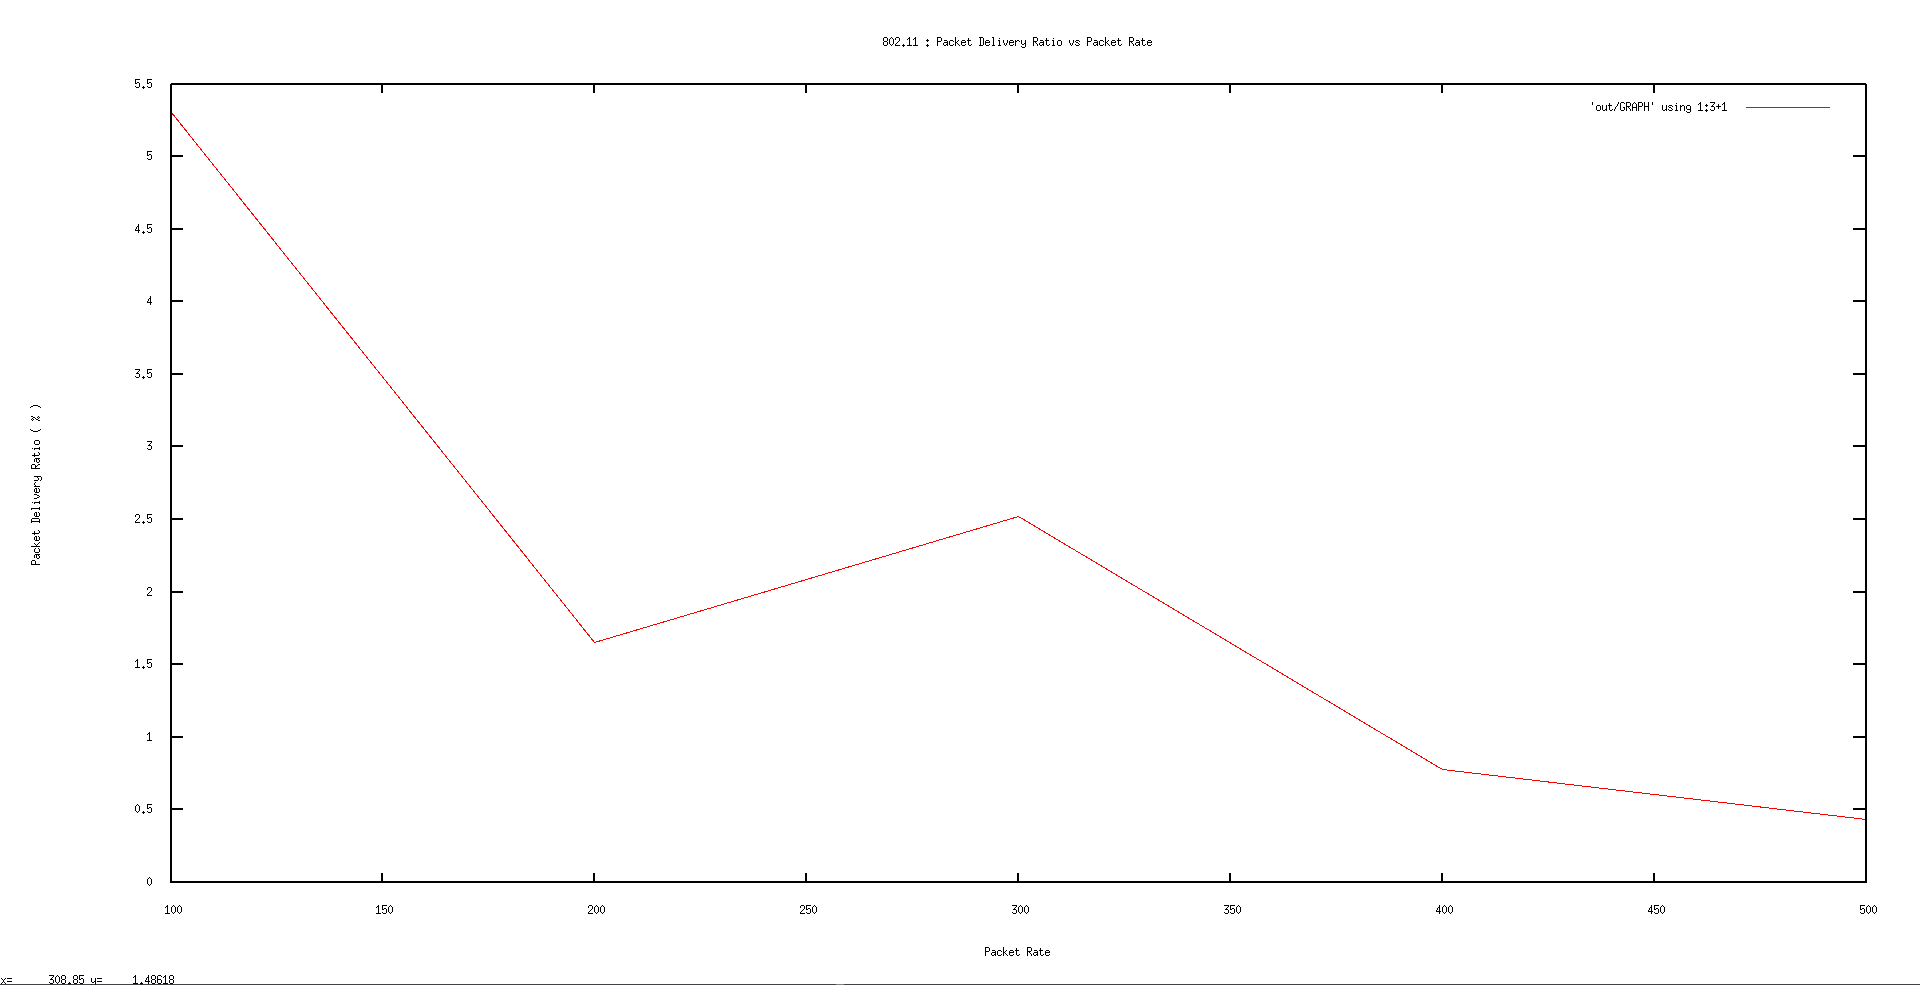
\includegraphics[scale=	0.26]{image/802.15.4/Packetdeliveryratio_vs_packetRates.png}
\end{figure}

\begin{figure}[H]
	\centering
	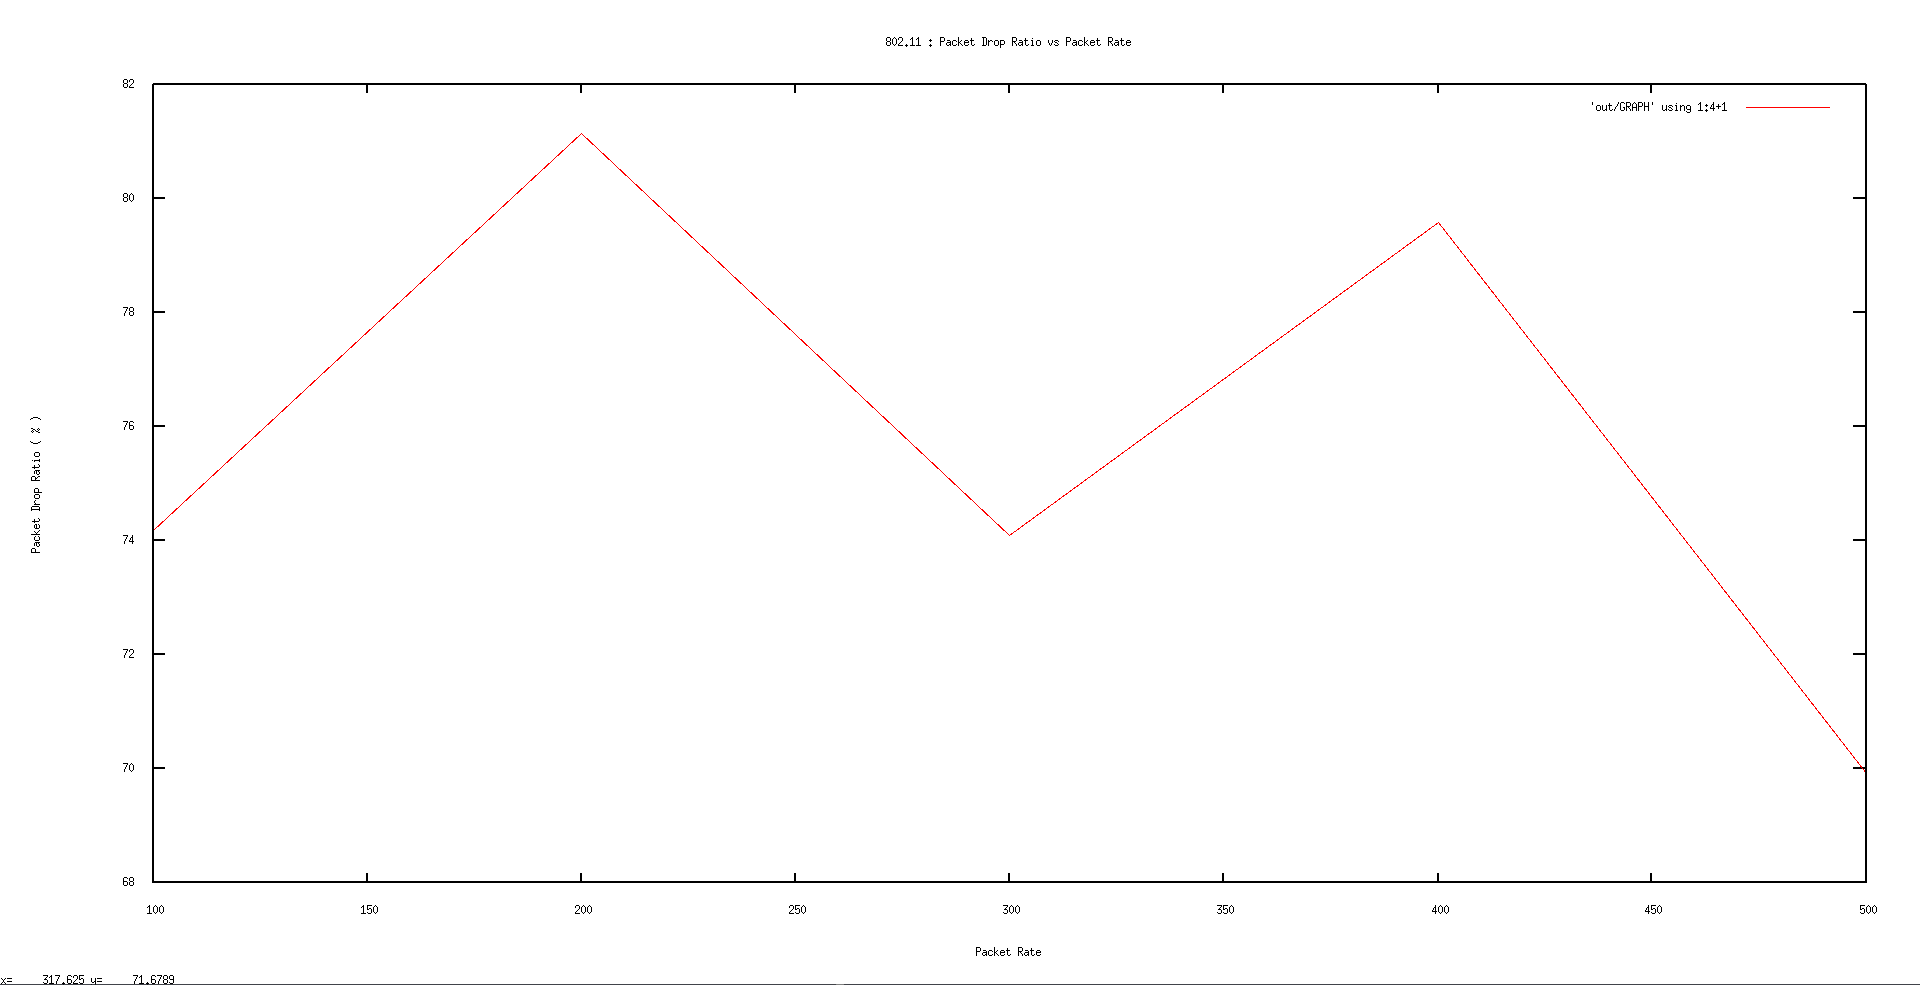
\includegraphics[scale=	0.26]{image/802.15.4/Packetdropratio_vs_packetRates.png}
\end{figure}

\newpage
\title{Variation in Coverage}
\begin{figure}[H]
	\centering
	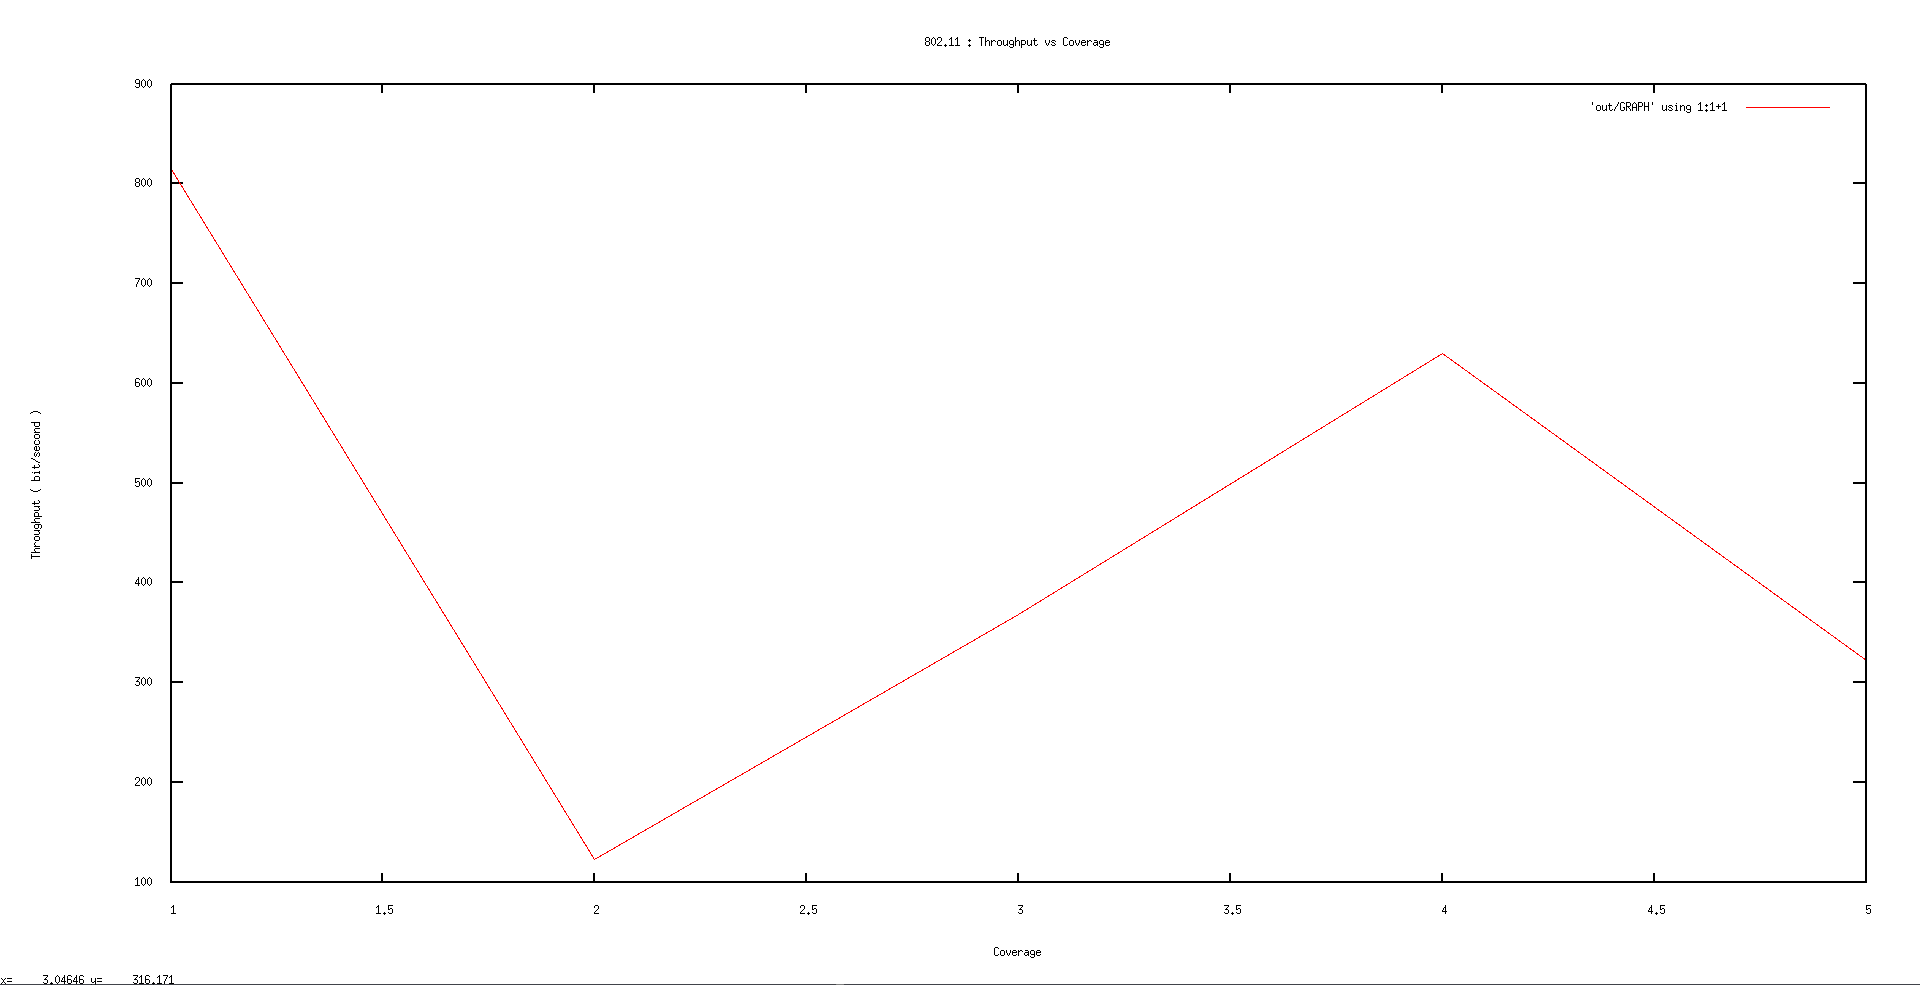
\includegraphics[scale=	0.26]{image/802.15.4/Throughput_vs_coverage.png}
\end{figure}

\begin{figure}[H]
	\centering
	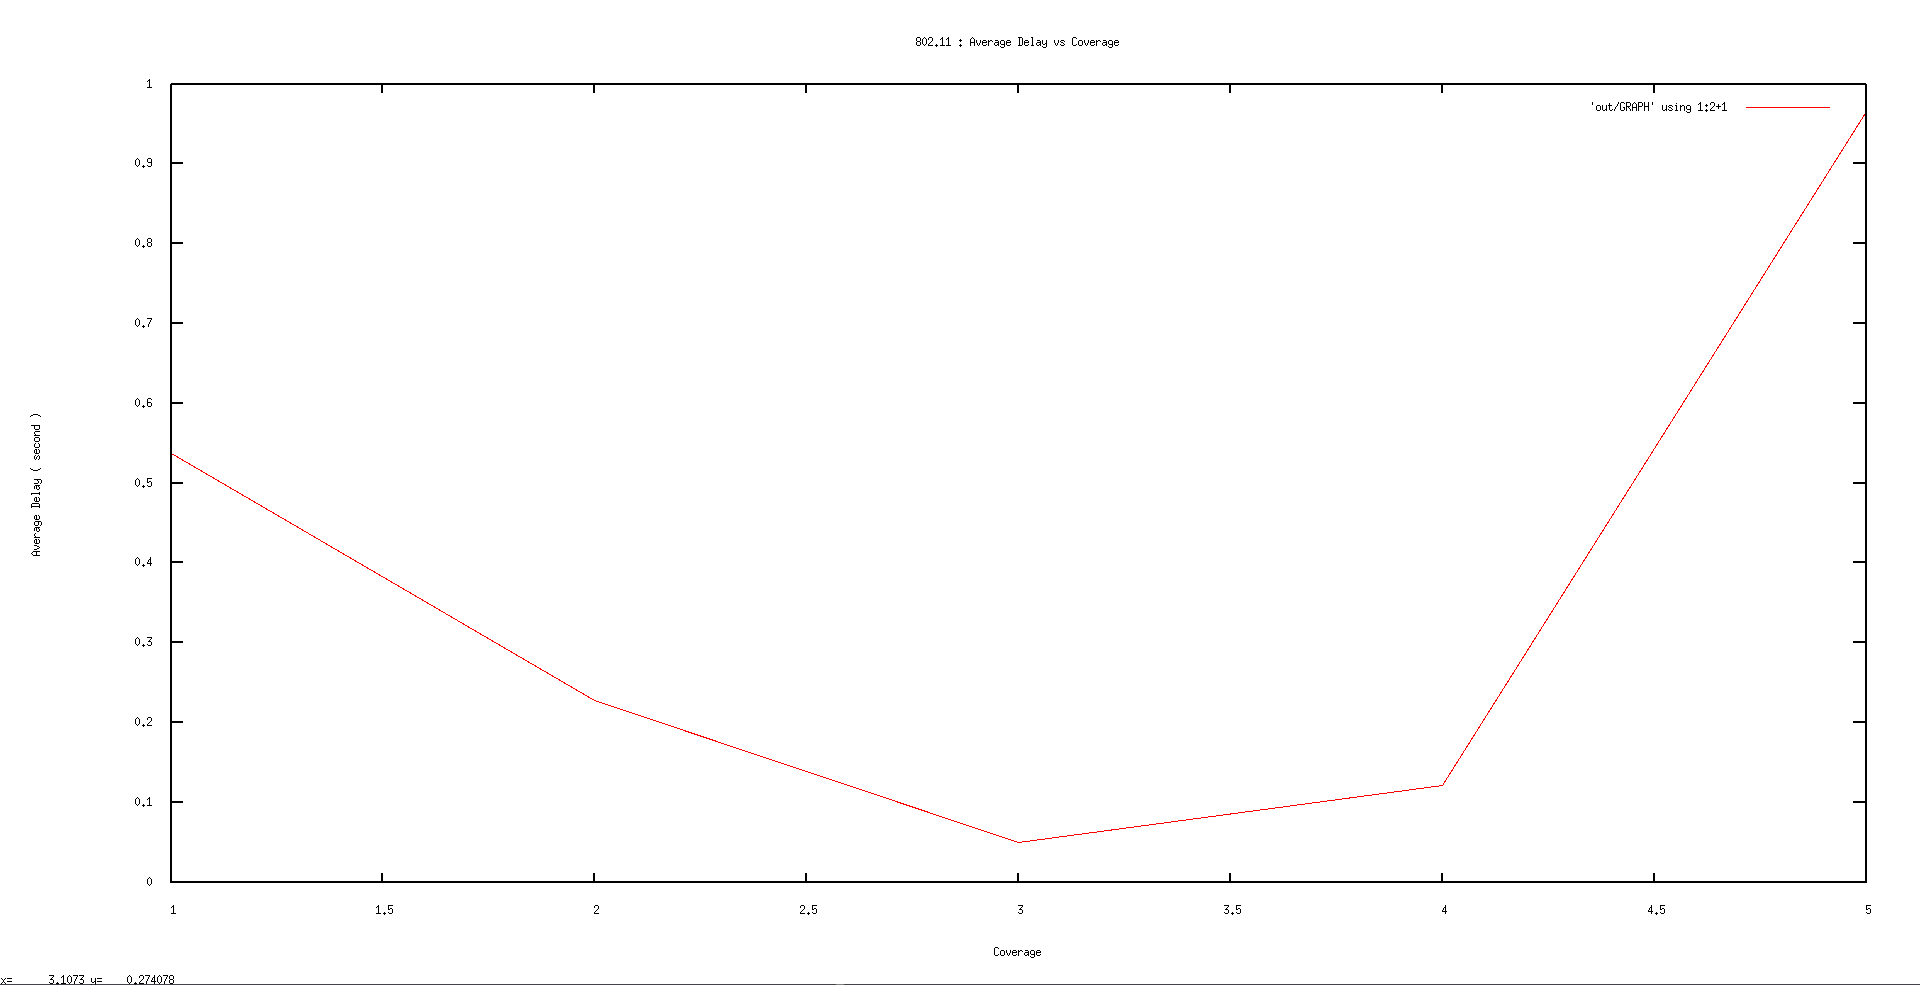
\includegraphics[scale=	0.26]{image/802.15.4/Averagedelay_vs_coverage.png}
\end{figure}

\begin{figure}[H]
	\centering
	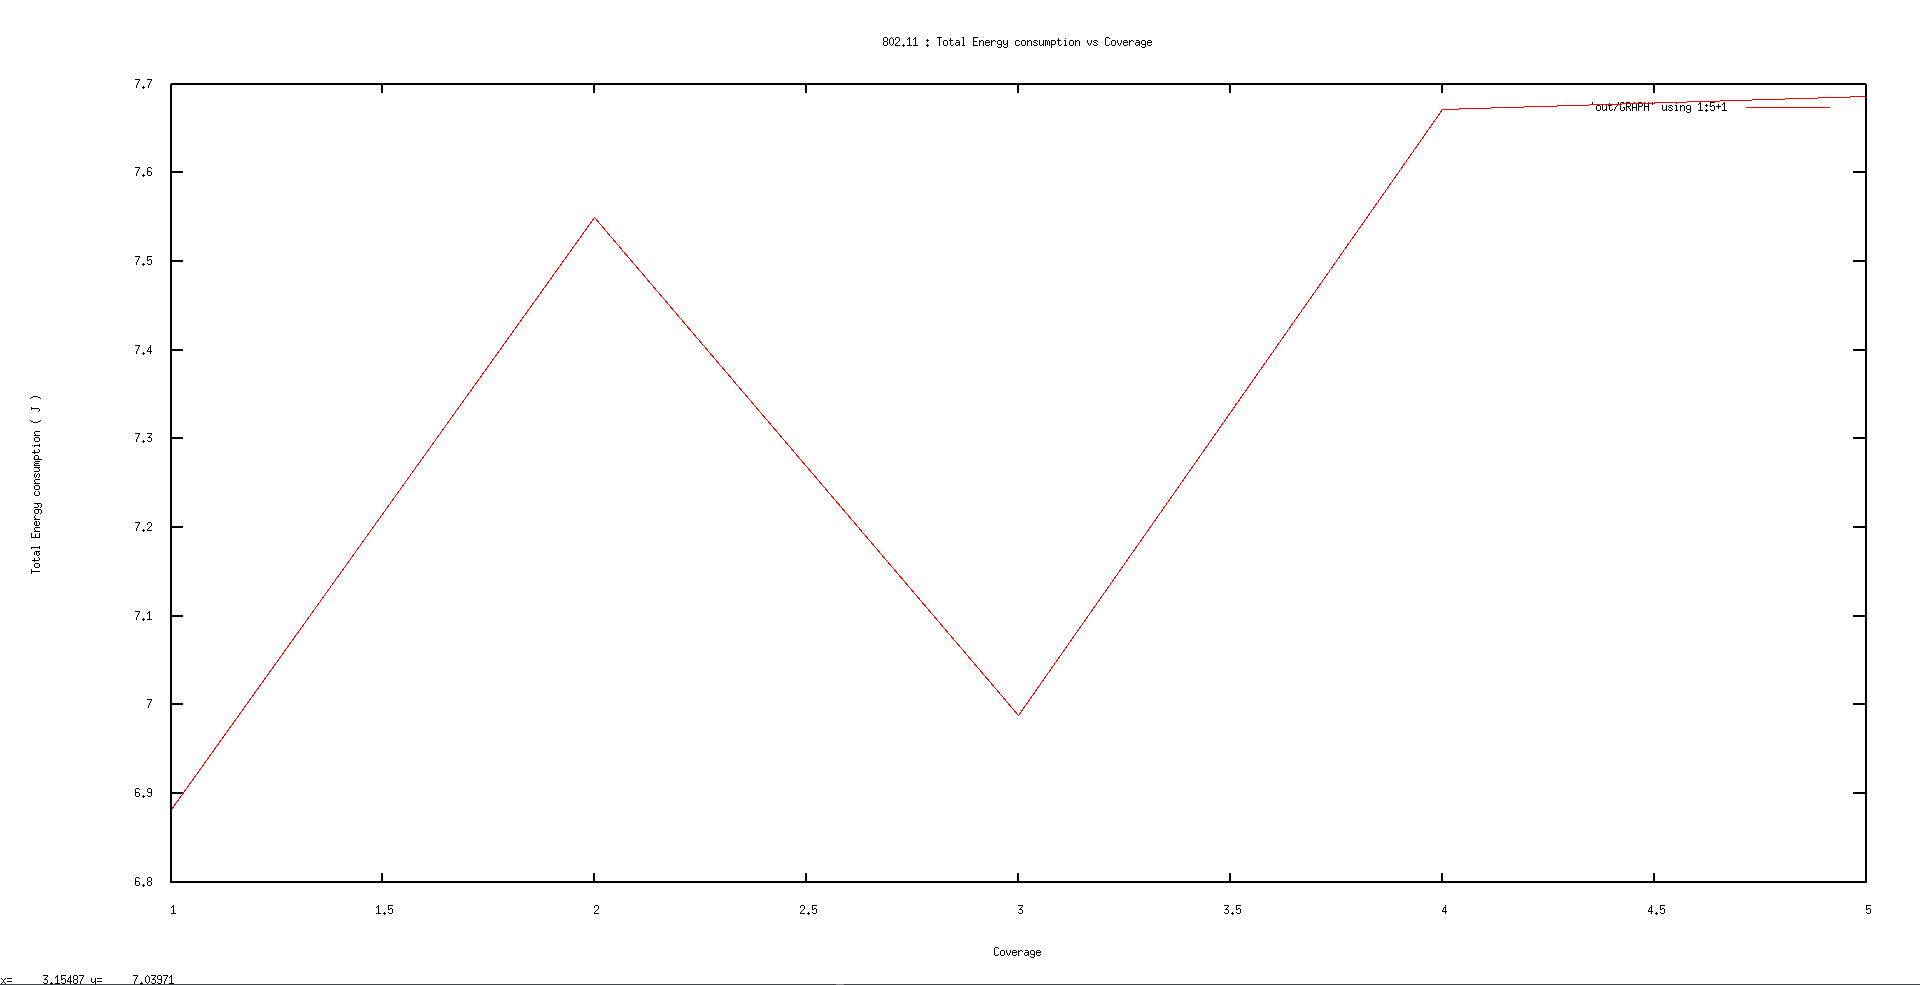
\includegraphics[scale=	0.26]{image/802.15.4/Energyconsumption_vs_coverage.png}
\end{figure}

\begin{figure}[H]
	\centering
	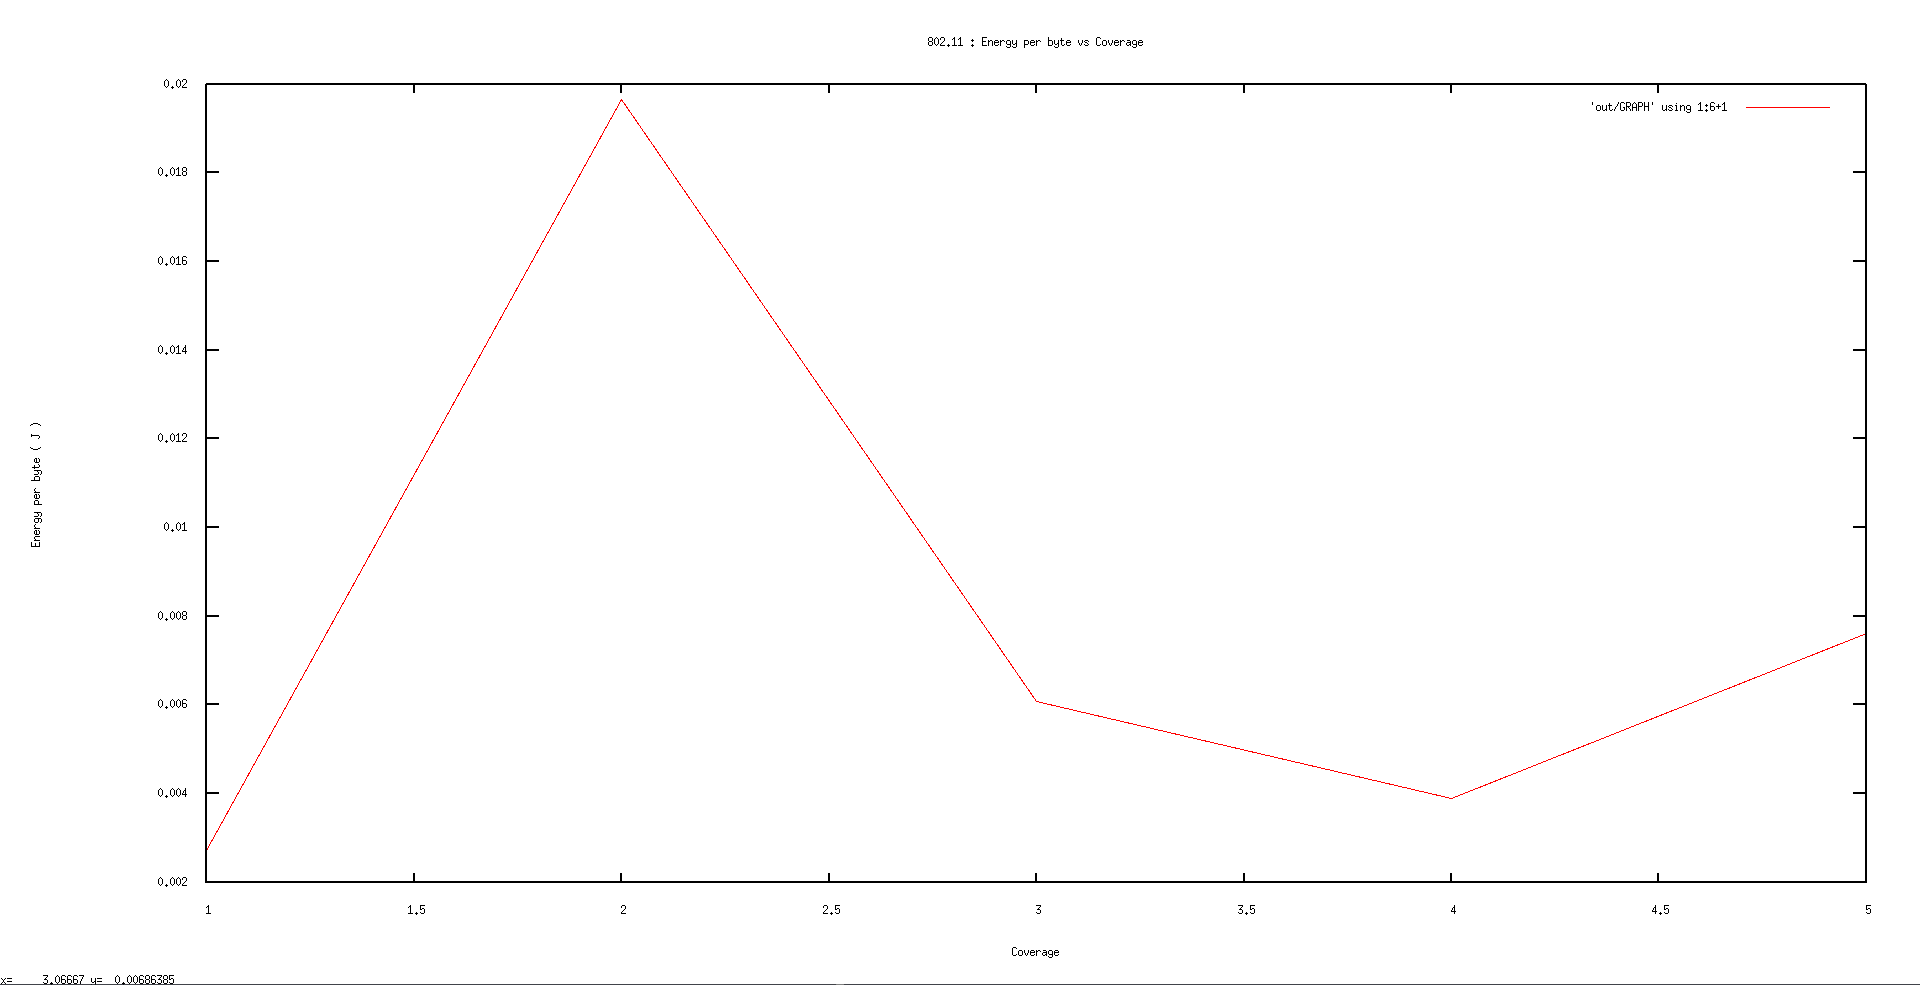
\includegraphics[scale=	0.26]{image/802.15.4/Energyperbytes_vs_coverage.png}
\end{figure}

\begin{figure}[H]
	\centering
	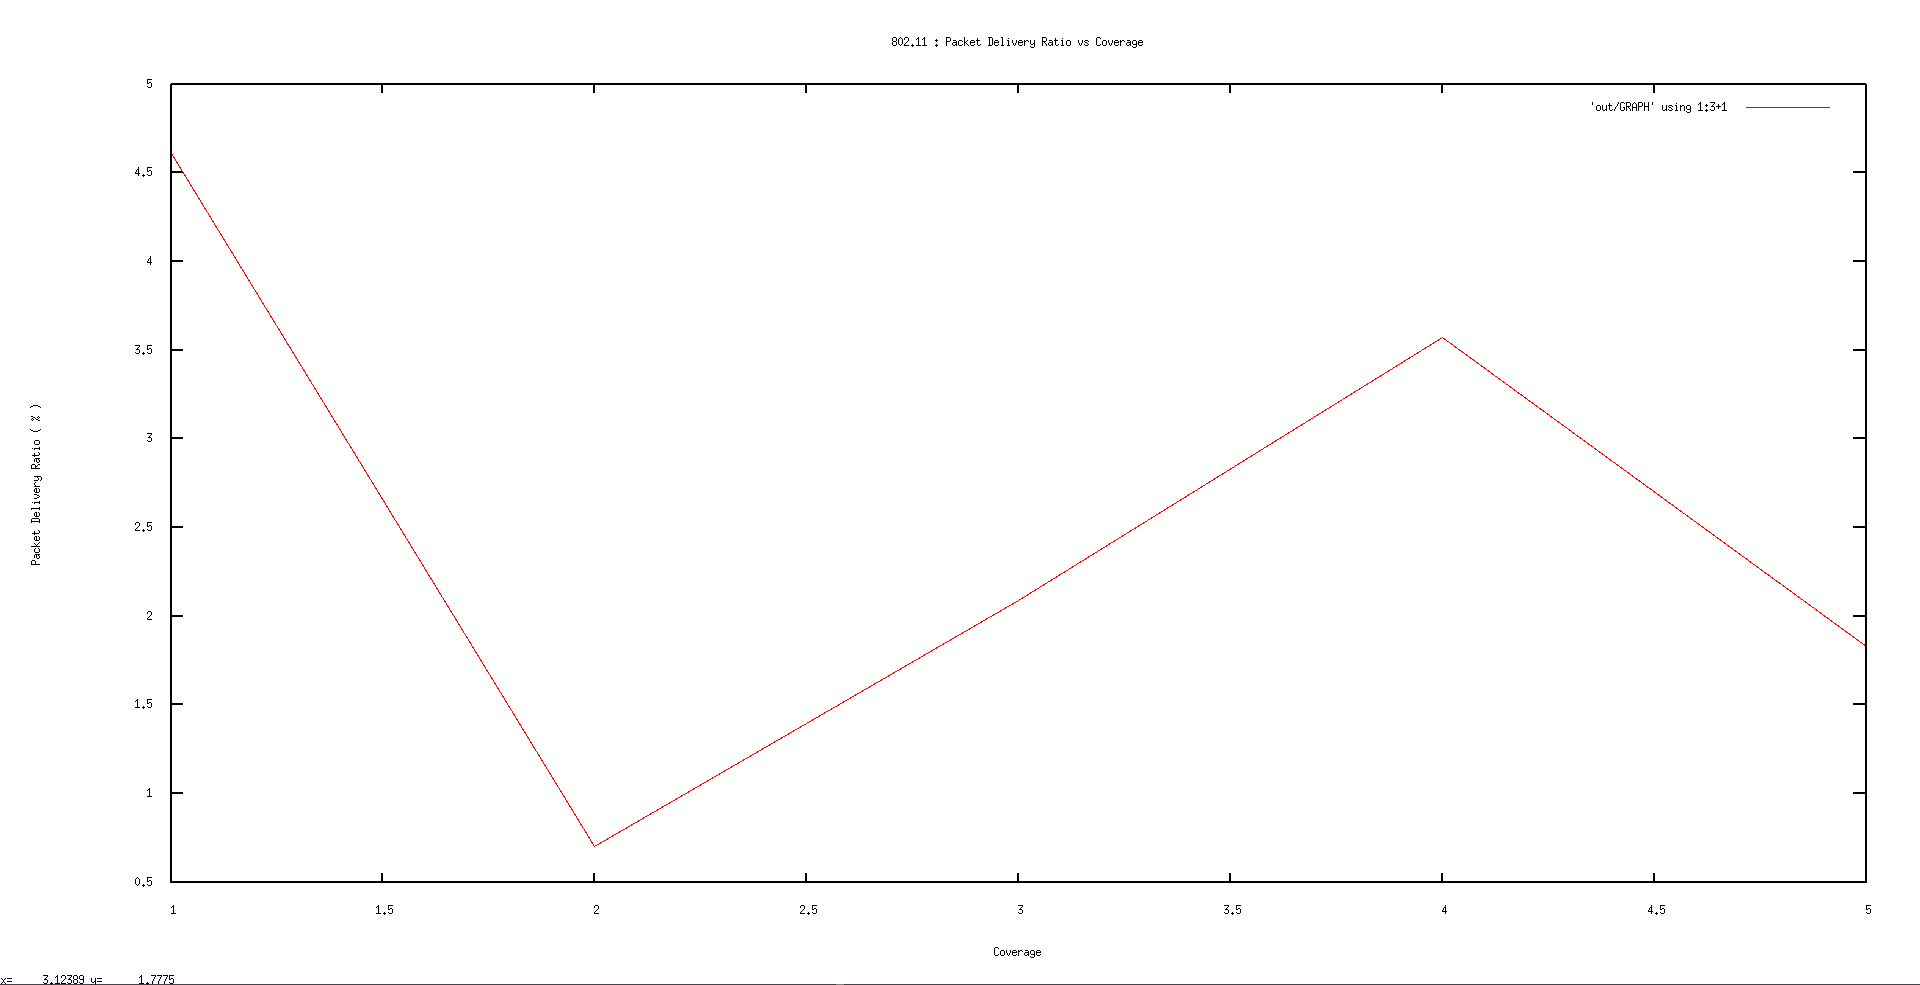
\includegraphics[scale=	0.26]{image/802.15.4/Packetdeliveryratio_vs_coverage.png}
\end{figure}

\begin{figure}[H]
	\centering
	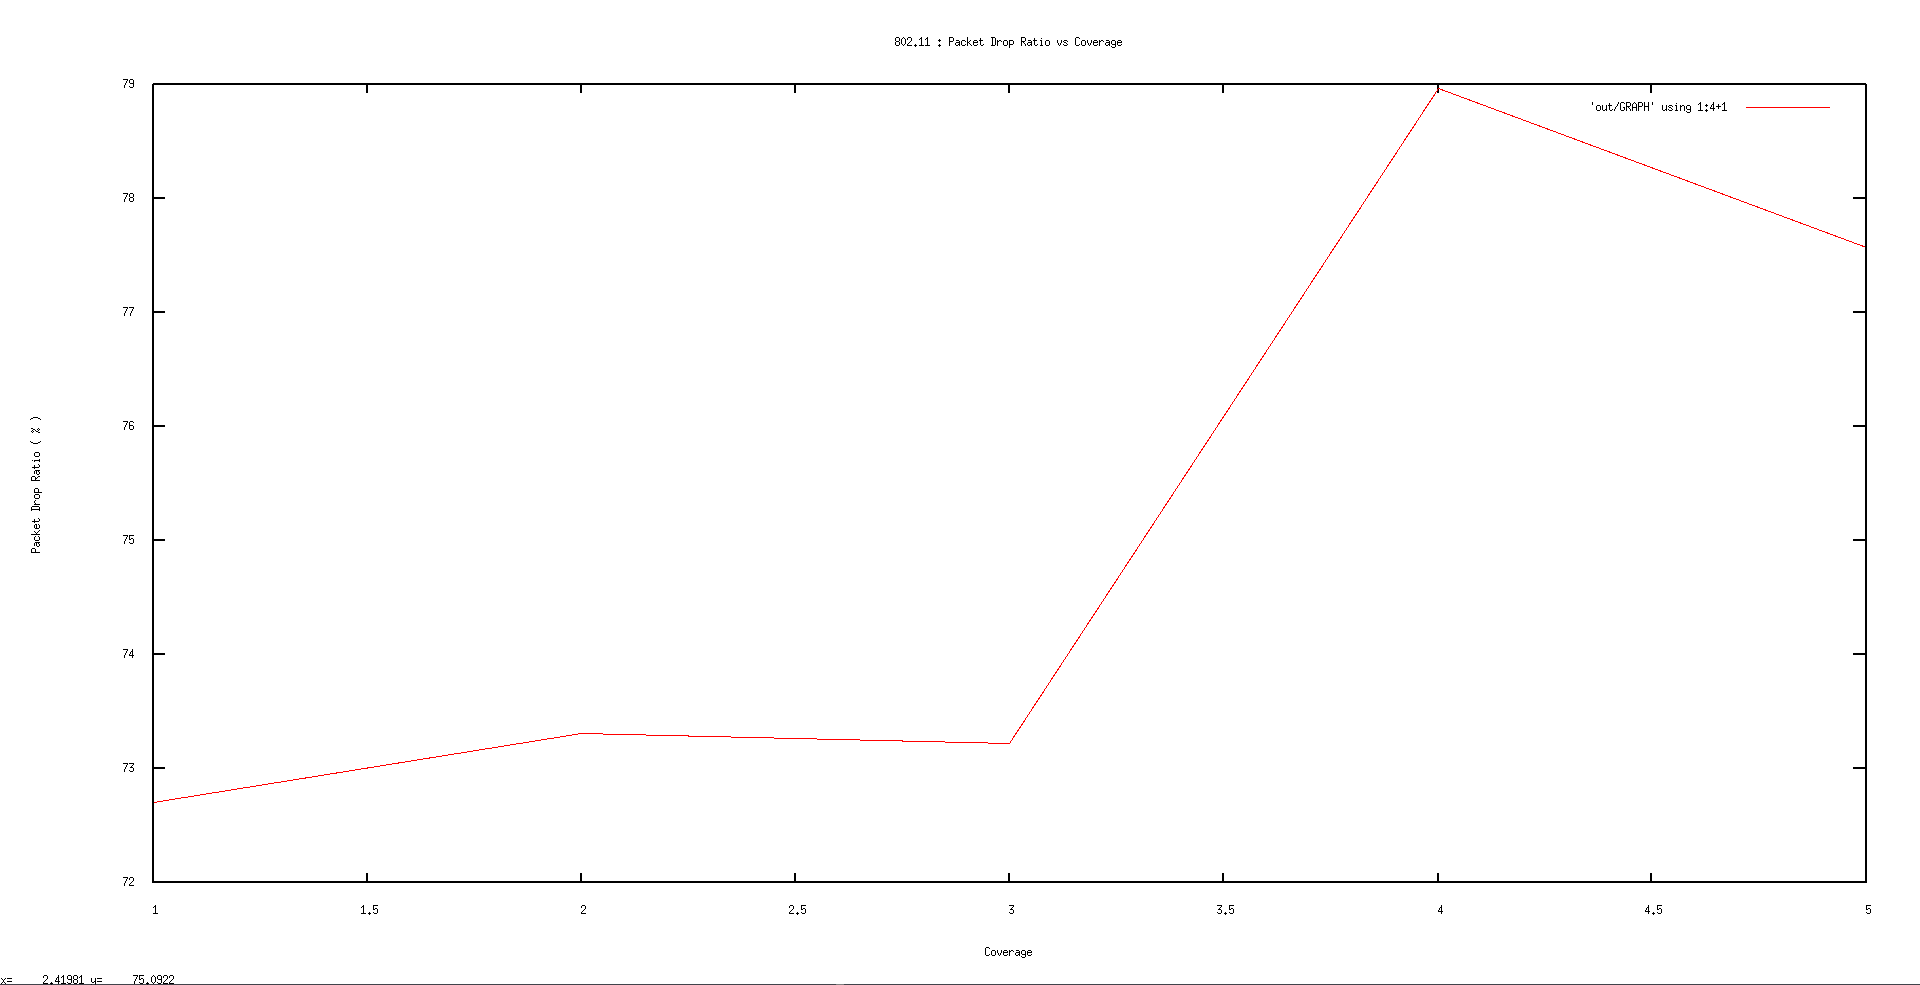
\includegraphics[scale=	0.26]{image/802.15.4/Packetdropratio_vs_coverage.png}
\end{figure}





\newpage
\section{Modification}

\subsection{Variation in flows}

\begin{figure}[H]
	\centering
	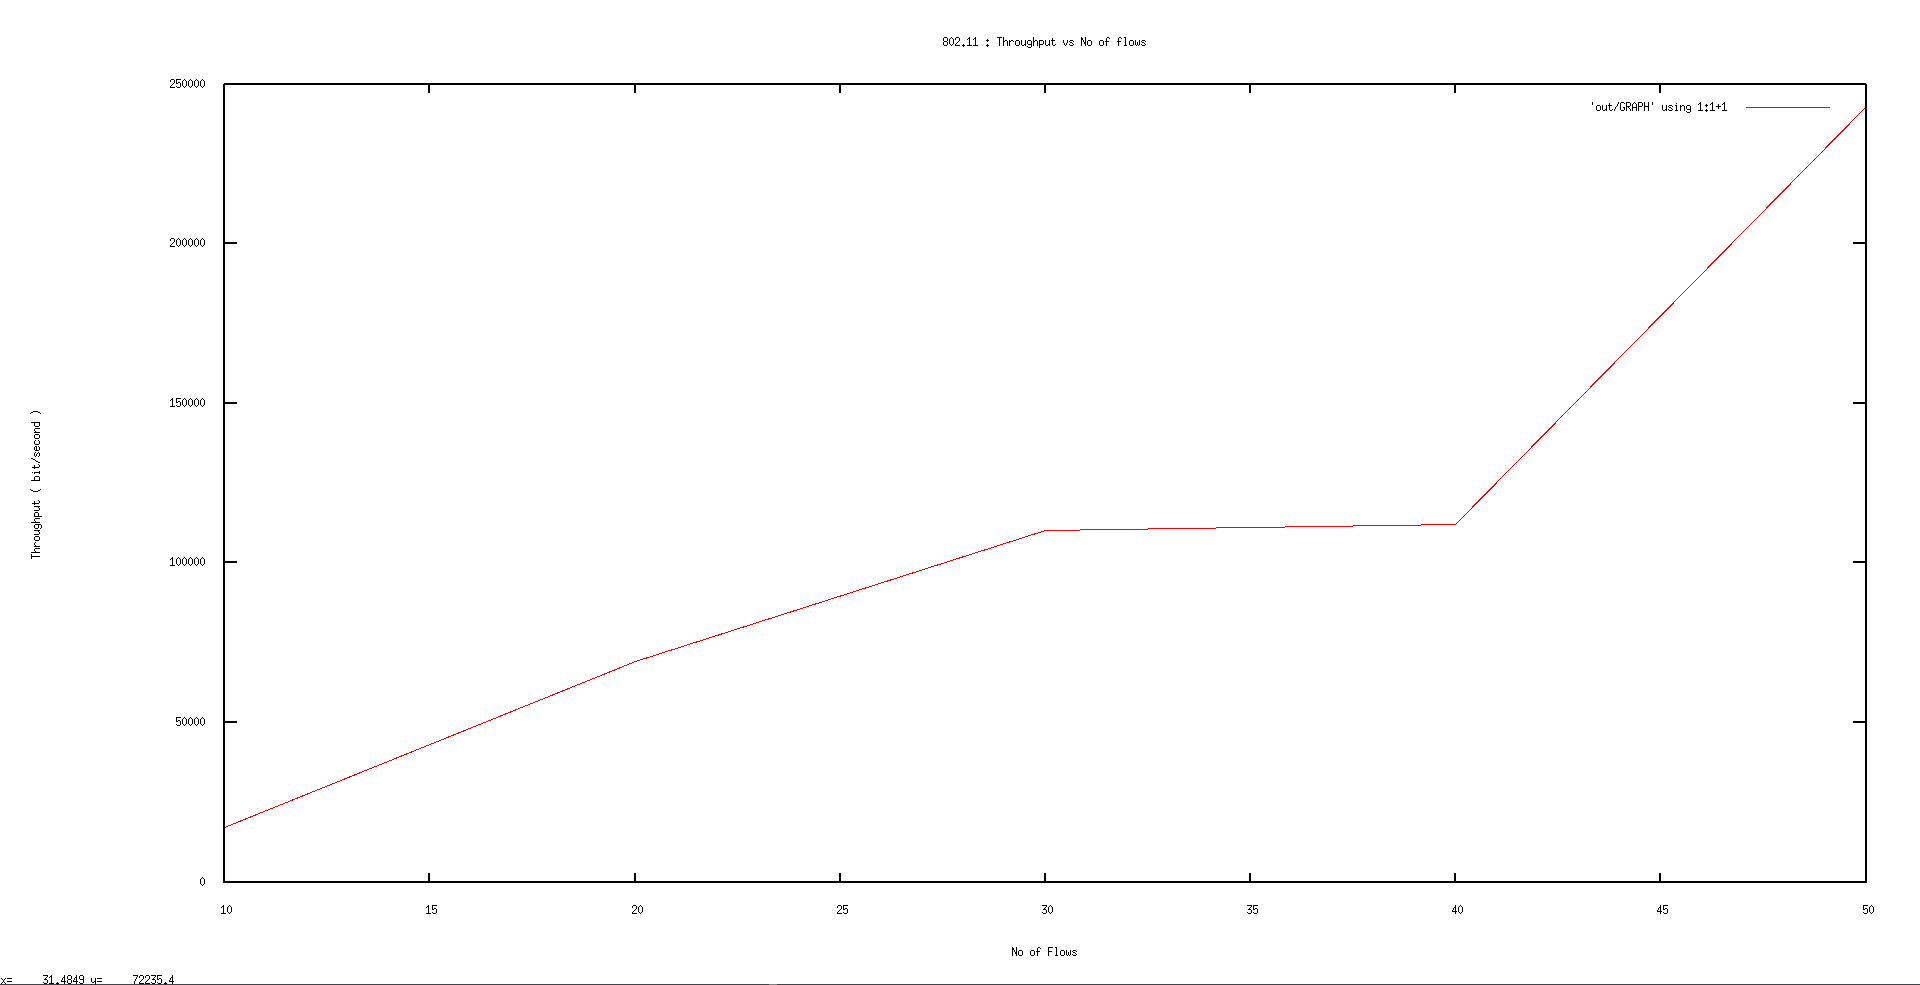
\includegraphics[scale=	0.26]{image/bpics/bm_Throughput_vs_flows.png}
\end{figure}

\begin{figure}[H]
	\centering
	\includegraphics[scale=	0.26]{image/apics/am_Throughput_vs_flows.png}
\end{figure}


\begin{figure}[H]
	\centering
	\includegraphics[scale=	0.26]{image/bpics/bm_averagedelay_vs_flows.png}
\end{figure}

\begin{figure}[H]
	\centering
	\includegraphics[scale=	0.26]{image/apics/am_averagedelay_vs_flows.png}
\end{figure}

\begin{figure}[H]
	\centering
	\includegraphics[scale=	0.26]{image/bpics/bm_energyperbyte_vs_flows.png}
\end{figure}

\begin{figure}[H]
	\centering
	\includegraphics[scale=	0.26]{image/apics/am_energyperbyte_vs_flows.png}
\end{figure}

\begin{figure}[H]
	\centering
	\includegraphics[scale=	0.26]{image/bpics/bm_energyconsumption_vs_flows.png}
\end{figure}

\begin{figure}[H]
	\centering
	\includegraphics[scale=	0.26]{image/apics/am_energyconsumption_vs_flows.png}
\end{figure}


\begin{figure}[H]
	\centering
	\includegraphics[scale=	0.26]{image/bpics/bm_packetdeliveryratio_vs_flows.png}
\end{figure}

\begin{figure}[H]
	\centering
	\includegraphics[scale=	0.26]{image/apics/am_packetdeliveryratio_vs_flows.png}
\end{figure}


\begin{figure}[H]
	\centering
	\includegraphics[scale=	0.26]{image/bpics/bm_packetdropratio_vs_flows.png}
\end{figure}

\begin{figure}[H]
	\centering
	\includegraphics[scale=	0.26]{image/apics/am_packetdropratio_vs_flows.png}
\end{figure}





\subsection{Variation in Nodes}
\newpage

\begin{figure}[H]
	\centering
	\includegraphics[scale=	0.26]{image/bpics/bm_Throughput_vs_nodes.png}
\end{figure}

\begin{figure}[H]
	\centering
	\includegraphics[scale=	0.26]{image/apics/am_Throughput_vs_nodes.png}
\end{figure}


\begin{figure}[H]
	\centering
	\includegraphics[scale=	0.26]{image/bpics/bm_averagedelay_vs_nodes.png}
\end{figure}

\begin{figure}[H]
	\centering
	\includegraphics[scale=	0.26]{image/apics/am_averagedelay_vs_nodes.png}
\end{figure}

\begin{figure}[H]
	\centering
	\includegraphics[scale=	0.26]{image/bpics/bm_energyperbyte_vs_nodes.png}
\end{figure}

\begin{figure}[H]
	\centering
	\includegraphics[scale=	0.26]{image/apics/am_energyperbyte_vs_nodes.png}
\end{figure}

\begin{figure}[H]
	\centering
	\includegraphics[scale=	0.26]{image/bpics/bm_energyconsumption_vs_nodes.png}
\end{figure}

\begin{figure}[H]
	\centering
	\includegraphics[scale=	0.26]{image/apics/am_energyconsumption_vs_nodes.png}
\end{figure}


\begin{figure}[H]
	\centering
	\includegraphics[scale=	0.26]{image/bpics/bm_packetdeliveryratio_vs_nodes.png}
\end{figure}

\begin{figure}[H]
	\centering
	\includegraphics[scale=	0.26]{image/apics/am_packetdeliveryratio_vs_nodes.png}
\end{figure}


\begin{figure}[H]
	\centering
	\includegraphics[scale=	0.26]{image/bpics/bm_packetdropratio_vs_nodes.png}
\end{figure}

\begin{figure}[H]
	\centering
	\includegraphics[scale=	0.26]{image/apics/am_packetdropratio_nodes.png}
\end{figure}



\subsection{Variation in Packet Rates}
\newpage

\begin{figure}[H]
	\centering
	\includegraphics[scale=	0.26]{image/bpics/bm_Throughput_vs_packetrates.png}
\end{figure}

\begin{figure}[H]
	\centering
	\includegraphics[scale=	0.26]{image/apics/am_Throughput_vs_packetrates.png}
\end{figure}


\begin{figure}[H]
	\centering
	\includegraphics[scale=	0.26]{image/bpics/bm_averagedelay_vs_packetrates.png}
\end{figure}

\begin{figure}[H]
	\centering
	\includegraphics[scale=	0.26]{image/apics/am_averagedeliveryratio_vs_packetrates.png}
\end{figure}

\begin{figure}[H]
	\centering
	\includegraphics[scale=	0.26]{image/bpics/bm_Energyperbyte_vs_packrates.png}
\end{figure}

\begin{figure}[H]
	\centering
	\includegraphics[scale=	0.26]{image/apics/am_energyperbyte_vs_packetrates.png}
\end{figure}

\begin{figure}[H]
	\centering
	\includegraphics[scale=	0.26]{image/bpics/bm_energyconsumption_vs_packetrates.png}
\end{figure}

\begin{figure}[H]
	\centering
	\includegraphics[scale=	0.26]{image/apics/am_energyconsumption_vs_packetrates.png}
\end{figure}


\begin{figure}[H]
	\centering
	\includegraphics[scale=	0.26]{image/bpics/bm_packetdeliveryratio_vs_packetrates.png}
\end{figure}

\begin{figure}[H]
	\centering
	\includegraphics[scale=	0.26]{image/apics/am_packetdeliveryratio_vs_packetrates.png}
\end{figure}


\begin{figure}[H]
	\centering
	\includegraphics[scale=	0.26]{image/bpics/bm_packetdropratio_vs_packetrates.png}
\end{figure}

\begin{figure}[H]
	\centering
	\includegraphics[scale=	0.26]{image/apics/am_packetdropratio_vs_packetrates.png}
\end{figure}





\subsection{Variation in Speed}
\newpage

\begin{figure}[H]
	\centering
	\includegraphics[scale=	0.26]{image/bpics/bm_Throughput_vs_speed.png}
\end{figure}

\begin{figure}[H]
	\centering
	\includegraphics[scale=	0.26]{image/apics/am_Throughput_vs_speed.png}
\end{figure}


\begin{figure}[H]
	\centering
	\includegraphics[scale=	0.26]{image/bpics/bm_averagedelay_vs_speed.png}
\end{figure}

\begin{figure}[H]
	\centering
	\includegraphics[scale=	0.26]{image/apics/am_averagedelay_vs_speed.png}
\end{figure}

\begin{figure}[H]
	\centering
	\includegraphics[scale=	0.26]{image/bpics/temp.png}
\end{figure}

\begin{figure}[H]
	\centering
	\includegraphics[scale=	0.26]{image/apics/am_energyperbyte_vs_speed.png}
\end{figure}

\begin{figure}[H]
	\centering
	\includegraphics[scale=	0.26]{image/bpics/bm_energyconsumption_vs_speed.png}
\end{figure}

\begin{figure}[H]
	\centering
	\includegraphics[scale=	0.26]{image/apics/am_energyconsumption_vs_speed.png}
\end{figure}


\begin{figure}[H]
	\centering
	\includegraphics[scale=	0.26]{image/bpics/bm_packetdeliveryratio_vs_speed.png}
\end{figure}

\begin{figure}[H]
	\centering
	\includegraphics[scale=	0.26]{image/apics/am_packetdeliveryratio_vs_speed.png}
\end{figure}


\begin{figure}[H]
	\centering
	\includegraphics[scale=	0.26]{image/bpics/bm_packetdropratio_vs_speed.png}
\end{figure}

\begin{figure}[H]
	\centering
	\includegraphics[scale=	0.26]{image/apics/am_packetdropratio_vs_speed.png}
\end{figure}








%---------------------------------------------------------------




%---------------------------------------------------------------
%summary
\newpage
\section{Summary Findings}
\begin{enumerate}
    \item Packet delivery ratio is much higher in 802.11 than 802.15.4. Not only that throughput is also greater.
    
    \item 802.15.4 works better when AODV is used
    \item The maximum application packet size in 
802.15.4 is 100 bytes. DSR adds larger overhead than AODV and hence 
makes the overall packet size larger than AODV does, so AODV works better
    
    \item The modification in DSDV that converted in to DVR proves that DSDV works better than DVR
    
    \item The modification in tcp.cc improves performance, retransmission of packet decreases
\end{enumerate}

%---------------------------------------------------------------

\end{document}